\documentclass[twoside]{article}

% Packages required by doxygen
\usepackage{fixltx2e}
\usepackage{calc}
\usepackage{doxygen}
\usepackage[export]{adjustbox} % also loads graphicx
\usepackage{graphicx}
\usepackage[utf8]{inputenc}
\usepackage{makeidx}
\usepackage{multicol}
\usepackage{multirow}
\PassOptionsToPackage{warn}{textcomp}
\usepackage{textcomp}
\usepackage[nointegrals]{wasysym}
\usepackage[table]{xcolor}

% Font selection
\usepackage[T1]{fontenc}
\usepackage[scaled=.90]{helvet}
\usepackage{courier}
\usepackage{amssymb}
\usepackage{sectsty}
\renewcommand{\familydefault}{\sfdefault}
\allsectionsfont{%
  \fontseries{bc}\selectfont%
  \color{darkgray}%
}
\renewcommand{\DoxyLabelFont}{%
  \fontseries{bc}\selectfont%
  \color{darkgray}%
}
\newcommand{\+}{\discretionary{\mbox{\scriptsize$\hookleftarrow$}}{}{}}

% Page & text layout
\usepackage{geometry}
\geometry{%
  a4paper,%
  top=2.5cm,%
  bottom=2.5cm,%
  left=2.5cm,%
  right=2.5cm%
}
\tolerance=750
\hfuzz=15pt
\hbadness=750
\setlength{\emergencystretch}{15pt}
\setlength{\parindent}{0cm}
\setlength{\parskip}{0.2cm}
\makeatletter
\renewcommand{\paragraph}{%
  \@startsection{paragraph}{4}{0ex}{-1.0ex}{1.0ex}{%
    \normalfont\normalsize\bfseries\SS@parafont%
  }%
}
\renewcommand{\subparagraph}{%
  \@startsection{subparagraph}{5}{0ex}{-1.0ex}{1.0ex}{%
    \normalfont\normalsize\bfseries\SS@subparafont%
  }%
}
\makeatother

% Headers & footers
\usepackage{fancyhdr}
\pagestyle{fancyplain}
\fancyhead[LE]{\fancyplain{}{\bfseries\thepage}}
\fancyhead[CE]{\fancyplain{}{}}
\fancyhead[RE]{\fancyplain{}{\bfseries\leftmark}}
\fancyhead[LO]{\fancyplain{}{\bfseries\rightmark}}
\fancyhead[CO]{\fancyplain{}{}}
\fancyhead[RO]{\fancyplain{}{\bfseries\thepage}}
\fancyfoot[LE]{\fancyplain{}{}}
\fancyfoot[CE]{\fancyplain{}{}}
\fancyfoot[RE]{\fancyplain{}{\bfseries\scriptsize Generated on Sat Dec 24 2016 16\+:10\+:36 for F\+C\+L\+I\+B -\/ v  -\/  Package by Doxygen }}
\fancyfoot[LO]{\fancyplain{}{\bfseries\scriptsize Generated on Sat Dec 24 2016 16\+:10\+:36 for F\+C\+L\+I\+B -\/ v  -\/  Package by Doxygen }}
\fancyfoot[CO]{\fancyplain{}{}}
\fancyfoot[RO]{\fancyplain{}{}}
\renewcommand{\footrulewidth}{0.4pt}
\renewcommand{\sectionmark}[1]{%
  \markright{\thesection\ #1}%
}

% Indices & bibliography
\usepackage{natbib}
\usepackage[titles]{tocloft}
\setcounter{tocdepth}{3}
\setcounter{secnumdepth}{5}
\makeindex

% Packages requested by user
\usepackage{amsmath}

% Hyperlinks (required, but should be loaded last)
\usepackage{ifpdf}
\ifpdf
  \usepackage[pdftex,pagebackref=true]{hyperref}
\else
  \usepackage[ps2pdf,pagebackref=true]{hyperref}
\fi
\hypersetup{%
  colorlinks=true,%
  linkcolor=blue,%
  citecolor=blue,%
  unicode%
}

% Custom commands
\newcommand{\clearemptydoublepage}{%
  \newpage{\pagestyle{empty}\cleardoublepage}%
}


%===== C O N T E N T S =====

\begin{document}

% Titlepage & ToC
\hypersetup{pageanchor=false,
             bookmarks=true,
             bookmarksnumbered=true,
             pdfencoding=unicode
            }
\pagenumbering{roman}
\begin{titlepage}
\vspace*{7cm}
\begin{center}%
{\Large F\+C\+L\+I\+B -\/ v -\/ Package }\\
\vspace*{1cm}
{\large Generated by Doxygen 1.8.10}\\
\vspace*{0.5cm}
{\small Sat Dec 24 2016 16:10:36}\\
\end{center}
\end{titlepage}
\tableofcontents
\pagenumbering{arabic}
\hypersetup{pageanchor=true}

%--- Begin generated contents ---
\section{Introduction}
\label{index}\hypertarget{index}{}\hypertarget{index_whatis}{}\subsection{What is F\+C\+L\+I\+B ?}\label{index_whatis}
F\+C\+L\+I\+B is 
\begin{DoxyItemize}
\item A open source collection of Frictional Contact (F\+C) problems stored in a specific \href{http://www.hdfgroup.org/HDF5/}{\tt H\+D\+F5 format } 
\item A open source light implementation of Input/\+Output functions in C Language to read and write problems  
\end{DoxyItemize}~\newline
\hypertarget{index_goals}{}\subsection{Goals of the project}\label{index_goals}
The goal of this work is to set up a collection of 2\+D and 3\+D Frictional Contact (F\+C) problems in order to


\begin{DoxyItemize}
\item set up a list of benchmarks  
\item provide a standard framework for testing available and new algorithms for solving discrete frictional contact problems  
\item share common formulations of problems in order to exchange data 
\end{DoxyItemize}~\newline
\hypertarget{index_References}{}\subsection{References}\label{index_References}
\href{https://hal.inria.fr/hal-00945820v2/document}{\tt Vincent Acary, Maurice Br\'{e}mond, Tomasz Koziara, Franck P\'{e}rignon. F\+C\+L\+I\+B\+: a collection of discrete 3\+D Frictional Contact problems. \mbox{[}Technical Report\mbox{]} R\+T-\/0444, I\+N\+R\+I\+A. 2014, pp.\+34.} ~\newline


~\newline
 \hypertarget{index_howtodownload}{}\subsection{How to download  ?}\label{index_howtodownload}
How to download sources files of the A\+P\+I? 
\begin{DoxyItemize}
\item latest version on \href{https://github.com/FrictionalContactLibrary/fclib}{\tt github Frictional\+Contact\+Library/fclib} 
\item \href{https://github.com/FrictionalContactLibrary/fclib/releases}{\tt releases } 
\end{DoxyItemize}

~\newline


How to download the collection of problems ? 
\begin{DoxyItemize}
\item The directory fclib/data/fclib-\/library contains the list of problem files of the library of tests in the file ls-\/\+Rl.\+txt 


\item The problem files are not stored in the github repository but there\+:  
\begin{DoxyItemize}
\item \href{http://faf.gforge.inria.fr/fclib-library/}{\tt Current versions of problems are there }  
\item \href{http://fclib.gforge.inria.fr/resources/}{\tt Old tagged versions are there } 
\end{DoxyItemize}
\item \hyperlink{problems_0_2}{F\+Clib collection v0.\+2}  
\end{DoxyItemize}see \hyperlink{download}{Download} section for other details ~\newline
\hypertarget{index_Wahtis}{}\subsection{What is a Frictional contact problem ?}\label{index_Wahtis}
A Frictional contact problem is algebraic problem obtained after possible time and space discretizations of problems of mechanics of solid involving contact and Coulomb\textquotesingle{}s friction. The mathematical structure of the problem is a second-\/order cone complementarity problem. For more details, you could have a look to the \href{doc/FCLib.pdf}{\tt fclib specifications }\hypertarget{index_Localfclib}{}\subsubsection{The local Frictional Contact problem with equality constraints}\label{index_Localfclib}
Given 
\begin{DoxyItemize}
\item a positive semi--definite matrix ${W} \in {\mathrm{I\!R}}^{m \times m}$ 
\item a matrix ${V} \in {\mathrm{I\!R}}^{m \times p}$ 
\item a matrix ${R} \in {\mathrm{I\!R}}^{p \times p}$ 
\item a vector $q \in {\mathrm{I\!R}}^{m}$, 
\item a vector $s \in {\mathrm{I\!R}}^{p}$, 
\item a vector of coefficients of friction $\mu \in {\mathrm{I\!R}}^{n_c}$ 
\end{DoxyItemize}the Mixed 3\+D\+F\+C problem is to find three vectors $u\in{\mathrm{I\!R}}^m$, $r\in {\mathrm{I\!R}}^m$ and $\lambda \in {\mathrm{I\!R}}^p$ denoted by $\mathrm{M3DFC}(R,V,W,q,s,\mu)$ such that \begin{eqnarray*}\label{eq:lcp1} \begin{cases} V^T {r} + R \lambda + s = 0 \\ \\ \hat u = W {r} + V\lambda + q +\left[ \left[\begin{array}{c} \mu^\alpha \|u^\alpha_T\|\\ 0 \\ 0 \end{array}\right]^T, \alpha = 1 \ldots n_c \right]^T \\ \\ K^\star_{\mu} \ni {\hat u} \perp r \in K_{\mu} \end{cases} \end{eqnarray*} where the Coulomb friction cone for a contact $\alpha$ is defined by \begin{eqnarray*} \label{eq:CCC} K _{\mu^\alpha}^{\alpha} = \{r^\alpha, \|r^\alpha_T \| \leq \mu^\alpha |r^\alpha_N| \} \end{eqnarray*} and the set $K^{\alpha,\star}_{\mu^\alpha}$ is its dual. \hypertarget{index_globalfclib}{}\subsubsection{The Global Frictional Contact problem with equality constraints}\label{index_globalfclib}
We are also dealing with global F\+C problem defined by

Given 
\begin{DoxyItemize}
\item a positive definite matrix ${M} \in {\mathrm{I\!R}}^{n \times n}$ 
\item a vector $ {f} \in {\mathrm{I\!R}}^n$, 
\item a matrix ${H} \in {\mathrm{I\!R}}^{n \times m}$ 
\item a matrix ${G} \in {\mathrm{I\!R}}^{n \times p}$ 
\item a vector $w \in {\mathrm{I\!R}}^{m}$, 
\item a vector $b \in {\mathrm{I\!R}}^{p}$, 
\item a vector of coefficients of friction $\mu \in {\mathrm{I\!R}}^{n_c}$ 
\end{DoxyItemize}the Global Mixed 3\+D\+F\+C problem is to find four vectors $ {v} \in {\mathrm{I\!R}}^n$, $u\in{\mathrm{I\!R}}^m$, $r\in {\mathrm{I\!R}}^m$ and $\lambda \in {\mathrm{I\!R}}^p$ denoted by $\mathrm{GM3DFC}(M,H,G,w,b,\mu)$ such that \begin{eqnarray*} \begin{cases} M v = {H} {r} + G\lambda + {f} \\ \\ G^T v +b =0 \\ \\ \hat u = H^T v + w +\left[ \left[\begin{array}{c} \mu \|u^\alpha_T\|\\ 0 \\ 0 \end{array}\right]^T, \alpha = 1 \ldots n_c \right]^T \\ \\ K^\star_{\mu} \ni {\hat u} \perp r \in K_{\mu} \end{cases} \end{eqnarray*} \hypertarget{index_without}{}\subsubsection{Problems without equality constraints}\label{index_without}
If the original problems do not contain inequality constraints, or if they are reduced, the problems do no have the variables $\lambda$ as unknowns and can be simplified. However, the storage in H\+D\+F5 file remains the same.\hypertarget{index_merit}{}\subsubsection{Merit functions.}\label{index_merit}
The A\+P\+I provides also some Merit functions which measures if one set of vectors satisfies the previous problems. 
\section{Download}
\label{download}
\hypertarget{download}{}

\begin{DoxyItemize}
\item \href{https://github.com/FrictionalContactLibrary/fclib}{\tt https\+://github.\+com/\+Frictional\+Contact\+Library/fclib \+: source of the reader/writer C A\+PI on github }  
\item \href{https://github.com/FrictionalContactLibrary/fclib-library}{\tt https\+://github.\+com/\+Frictional\+Contact\+Library/fclib-\/library \+: The collection of problems with the help of git-\/lfs }  
\item \href{https://github.com/FrictionalContactLibrary/fclib-scripts}{\tt https\+://github.\+com/\+Frictional\+Contact\+Library/fclib-\/scripts \+: Some scripts that generate the problems }  
\end{DoxyItemize}
\section{Contact us}
\label{contact}
\hypertarget{contact}{}
For any information or help, send an email to  
\section{Related Publications}
\label{publications}
\hypertarget{publications}{}
\href{https://hal.inria.fr/hal-00945820v2/document}{\tt Vincent Acary, Maurice Br\'{e}mond, Tomasz Koziara, Franck P\'{e}rignon. F\+C\+L\+I\+B\+: a collection of discrete 3\+D Frictional Contact problems. \mbox{[}Technical Report\mbox{]} R\+T-\/0444, I\+N\+R\+I\+A. 2014, pp.\+34.} ~\newline


~\newline
 

~\newline
 
\section{Class Index}
\subsection{Class List}
Here are the classes, structs, unions and interfaces with brief descriptions\+:\begin{DoxyCompactList}
\item\contentsline{section}{\mbox{\hyperlink{structfclib__global}{fclib\+\_\+global}} \\*The global frictional contact problem defined by }{\pageref{structfclib__global}}{}
\item\contentsline{section}{\mbox{\hyperlink{structfclib__info}{fclib\+\_\+info}} \\*This structure allows the user to enter a problem information as a title, a short description and known mathematical properties of the problem }{\pageref{structfclib__info}}{}
\item\contentsline{section}{\mbox{\hyperlink{structfclib__local}{fclib\+\_\+local}} \\*The local frictional contact problem defined by }{\pageref{structfclib__local}}{}
\item\contentsline{section}{\mbox{\hyperlink{structfclib__matrix}{fclib\+\_\+matrix}} \\*Matrix in compressed row/column or triplet form }{\pageref{structfclib__matrix}}{}
\item\contentsline{section}{\mbox{\hyperlink{structfclib__matrix__info}{fclib\+\_\+matrix\+\_\+info}} \\*This structure allows the user to enter a description for a given matrix (comment, conditionning, determinant, rank.) if they are known }{\pageref{structfclib__matrix__info}}{}
\item\contentsline{section}{\mbox{\hyperlink{structfclib__solution}{fclib\+\_\+solution}} \\*A solution or a guess for the frictional contact problem }{\pageref{structfclib__solution}}{}
\end{DoxyCompactList}

\section{File Index}
\subsection{File List}
Here is a list of all files with brief descriptions\+:\begin{DoxyCompactList}
\item\contentsline{section}{\mbox{\hyperlink{additionalpages_8doxygen}{additionalpages.\+doxygen}} }{\pageref{additionalpages_8doxygen}}{}
\item\contentsline{section}{\mbox{\hyperlink{fclib_8c}{fclib.\+c}} }{\pageref{fclib_8c}}{}
\item\contentsline{section}{\mbox{\hyperlink{fclib_8h}{fclib.\+h}} }{\pageref{fclib_8h}}{}
\item\contentsline{section}{\mbox{\hyperlink{fctst_8c}{fctst.\+c}} }{\pageref{fctst_8c}}{}
\item\contentsline{section}{\mbox{\hyperlink{fctst__merit_8c}{fctst\+\_\+merit.\+c}} }{\pageref{fctst__merit_8c}}{}
\item\contentsline{section}{\mbox{\hyperlink{mainpage_8doxygen}{mainpage.\+doxygen}} }{\pageref{mainpage_8doxygen}}{}
\end{DoxyCompactList}

\section{Class Documentation}
\hypertarget{structfclib__global}{}\subsection{fclib\+\_\+global Struct Reference}
\label{structfclib__global}\index{fclib\+\_\+global@{fclib\+\_\+global}}


The global frictional contact problem defined by.  




{\ttfamily \#include $<$fclib.\+h$>$}



Collaboration diagram for fclib\+\_\+global\+:\nopagebreak
\begin{figure}[H]
\begin{center}
\leavevmode
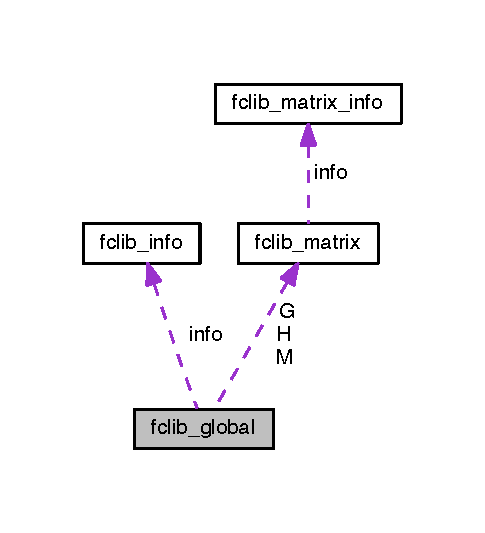
\includegraphics[width=233pt]{structfclib__global__coll__graph}
\end{center}
\end{figure}
\subsubsection*{Public Attributes}
\begin{DoxyCompactItemize}
\item 
struct \hyperlink{structfclib__matrix}{fclib\+\_\+matrix} $\ast$ \hyperlink{structfclib__global_a82538cefd07d0f1f6c1e7baebe768fc6}{M}
\begin{DoxyCompactList}\small\item\em the matrix M (see mathematical description below) \end{DoxyCompactList}\item 
struct \hyperlink{structfclib__matrix}{fclib\+\_\+matrix} $\ast$ \hyperlink{structfclib__global_ac87d5553d144625b9006e2e8b0c89b3c}{H}
\begin{DoxyCompactList}\small\item\em the matrix M (see mathematical description below) \end{DoxyCompactList}\item 
struct \hyperlink{structfclib__matrix}{fclib\+\_\+matrix} $\ast$ \hyperlink{structfclib__global_a897c09aca4a010076ed9ddb3f7527a79}{G}
\begin{DoxyCompactList}\small\item\em the matrix M (see mathematical description below) \end{DoxyCompactList}\item 
double $\ast$ \hyperlink{structfclib__global_a99fd8c775c35a6a0e233df1f8cae181a}{mu}
\begin{DoxyCompactList}\small\item\em the vector $\mu$ of coefficient of friction (see mathematical description below) \end{DoxyCompactList}\item 
double $\ast$ \hyperlink{structfclib__global_a6d5d0d1f9169b886eb3d3aca0632e8a9}{f}
\begin{DoxyCompactList}\small\item\em the vector f (see mathematical description below) \end{DoxyCompactList}\item 
double $\ast$ \hyperlink{structfclib__global_a1badf3df92b120566a2ee3c42194972f}{b}
\begin{DoxyCompactList}\small\item\em the vector b (see mathematical description below) \end{DoxyCompactList}\item 
double $\ast$ \hyperlink{structfclib__global_a8b175716b6c1f84509cf44b36a76e7ca}{w}
\begin{DoxyCompactList}\small\item\em the vector w (see mathematical description below) \end{DoxyCompactList}\item 
int \hyperlink{structfclib__global_a86dac5928d2c652f15ac688df14989a0}{spacedim}
\begin{DoxyCompactList}\small\item\em the dimension , 2 or 3, of the local space at contact (2d or 3d friction contact laws) \end{DoxyCompactList}\item 
struct \hyperlink{structfclib__info}{fclib\+\_\+info} $\ast$ \hyperlink{structfclib__global_aa6b4e80afc92dd1a9b260ff3a096b352}{info}
\begin{DoxyCompactList}\small\item\em info on the problem \end{DoxyCompactList}\end{DoxyCompactItemize}


\subsubsection{Detailed Description}
The global frictional contact problem defined by. 

Given 
\begin{DoxyItemize}
\item a symmetric positive definite matrix ${M} \in {\mathrm{I\!R}}^{n \times n}$ 
\item a vector $ {f} \in {\mathrm{I\!R}}^n$, 
\item a matrix ${H} \in {\mathrm{I\!R}}^{n \times m}$ 
\item a matrix ${G} \in {\mathrm{I\!R}}^{n \times p}$ 
\item a vector $w \in {\mathrm{I\!R}}^{m}$, 
\item a vector $b \in {\mathrm{I\!R}}^{p}$, 
\item a vector of coefficients of friction $\mu \in {\mathrm{I\!R}}^{n_c}$ 
\end{DoxyItemize}the Global Mixed 3\+D\+F\+C problem is to find four vectors $ {v} \in {\mathrm{I\!R}}^n$, $u\in{\mathrm{I\!R}}^m$, $r\in {\mathrm{I\!R}}^m$ and $\lambda \in {\mathrm{I\!R}}^p$ denoted by $\mathrm{GM3DFC}(M,H,G,w,b,\mu)$ such that \begin{eqnarray*} \begin{cases} M v = {H} {r} + G\lambda + {f} \\ \ \ G^T v +b =0 \\ \ \ \hat u = H^T v + w +\left[ \left[\begin{array}{c} \mu \|u^\alpha_T\|\ \ 0 \ \ 0 \end{array}\right]^T, \alpha = 1 \ldots n_c \right]^T \\ \ \ C^\star_{\mu} \ni {\hat u} \perp r \in C_{\mu} \end{cases} \end{eqnarray*} where the Coulomb friction cone for a contact $\alpha$ is defined by \begin{eqnarray*} \label{eq:CCC} C_{\mu^\alpha}^{\alpha} = \{r^\alpha, \|r^\alpha_T \| \leq \mu^\alpha |r^\alpha_N| \} *\end{eqnarray*} and the set $C^{\alpha,\star}_{\mu^\alpha}$ is its dual. 

Definition at line 174 of file fclib.\+h.



\subsubsection{Member Data Documentation}
\hypertarget{structfclib__global_a82538cefd07d0f1f6c1e7baebe768fc6}{}\index{fclib\+\_\+global@{fclib\+\_\+global}!M@{M}}
\index{M@{M}!fclib\+\_\+global@{fclib\+\_\+global}}
\paragraph[{M}]{\setlength{\rightskip}{0pt plus 5cm}struct {\bf fclib\+\_\+matrix}$\ast$ fclib\+\_\+global\+::\+M}\label{structfclib__global_a82538cefd07d0f1f6c1e7baebe768fc6}


the matrix M (see mathematical description below) 



Definition at line 177 of file fclib.\+h.



Referenced by compare\+\_\+global\+\_\+problems(), fclib\+\_\+delete\+\_\+global(), fclib\+\_\+read\+\_\+global(), fclib\+\_\+write\+\_\+global(), main(), random\+\_\+global\+\_\+problem(), random\+\_\+global\+\_\+solutions(), read\+\_\+global\+\_\+vectors(), and write\+\_\+global\+\_\+vectors().

\hypertarget{structfclib__global_ac87d5553d144625b9006e2e8b0c89b3c}{}\index{fclib\+\_\+global@{fclib\+\_\+global}!H@{H}}
\index{H@{H}!fclib\+\_\+global@{fclib\+\_\+global}}
\paragraph[{H}]{\setlength{\rightskip}{0pt plus 5cm}struct {\bf fclib\+\_\+matrix}$\ast$ fclib\+\_\+global\+::\+H}\label{structfclib__global_ac87d5553d144625b9006e2e8b0c89b3c}


the matrix M (see mathematical description below) 



Definition at line 179 of file fclib.\+h.



Referenced by compare\+\_\+global\+\_\+problems(), fclib\+\_\+delete\+\_\+global(), fclib\+\_\+read\+\_\+global(), fclib\+\_\+write\+\_\+global(), main(), random\+\_\+global\+\_\+problem(), random\+\_\+global\+\_\+solutions(), read\+\_\+global\+\_\+vectors(), and write\+\_\+global\+\_\+vectors().

\hypertarget{structfclib__global_a897c09aca4a010076ed9ddb3f7527a79}{}\index{fclib\+\_\+global@{fclib\+\_\+global}!G@{G}}
\index{G@{G}!fclib\+\_\+global@{fclib\+\_\+global}}
\paragraph[{G}]{\setlength{\rightskip}{0pt plus 5cm}struct {\bf fclib\+\_\+matrix}$\ast$ fclib\+\_\+global\+::\+G}\label{structfclib__global_a897c09aca4a010076ed9ddb3f7527a79}


the matrix M (see mathematical description below) 



Definition at line 181 of file fclib.\+h.



Referenced by compare\+\_\+global\+\_\+problems(), fclib\+\_\+delete\+\_\+global(), fclib\+\_\+read\+\_\+global(), fclib\+\_\+write\+\_\+global(), main(), random\+\_\+global\+\_\+problem(), random\+\_\+global\+\_\+solutions(), read\+\_\+global\+\_\+vectors(), and write\+\_\+global\+\_\+vectors().

\hypertarget{structfclib__global_a99fd8c775c35a6a0e233df1f8cae181a}{}\index{fclib\+\_\+global@{fclib\+\_\+global}!mu@{mu}}
\index{mu@{mu}!fclib\+\_\+global@{fclib\+\_\+global}}
\paragraph[{mu}]{\setlength{\rightskip}{0pt plus 5cm}double$\ast$ fclib\+\_\+global\+::mu}\label{structfclib__global_a99fd8c775c35a6a0e233df1f8cae181a}


the vector $\mu$ of coefficient of friction (see mathematical description below) 



Definition at line 183 of file fclib.\+h.



Referenced by compare\+\_\+global\+\_\+problems(), fclib\+\_\+delete\+\_\+global(), random\+\_\+global\+\_\+problem(), read\+\_\+global\+\_\+vectors(), and write\+\_\+global\+\_\+vectors().

\hypertarget{structfclib__global_a6d5d0d1f9169b886eb3d3aca0632e8a9}{}\index{fclib\+\_\+global@{fclib\+\_\+global}!f@{f}}
\index{f@{f}!fclib\+\_\+global@{fclib\+\_\+global}}
\paragraph[{f}]{\setlength{\rightskip}{0pt plus 5cm}double$\ast$ fclib\+\_\+global\+::f}\label{structfclib__global_a6d5d0d1f9169b886eb3d3aca0632e8a9}


the vector f (see mathematical description below) 



Definition at line 185 of file fclib.\+h.



Referenced by compare\+\_\+global\+\_\+problems(), fclib\+\_\+delete\+\_\+global(), random\+\_\+global\+\_\+problem(), read\+\_\+global\+\_\+vectors(), and write\+\_\+global\+\_\+vectors().

\hypertarget{structfclib__global_a1badf3df92b120566a2ee3c42194972f}{}\index{fclib\+\_\+global@{fclib\+\_\+global}!b@{b}}
\index{b@{b}!fclib\+\_\+global@{fclib\+\_\+global}}
\paragraph[{b}]{\setlength{\rightskip}{0pt plus 5cm}double$\ast$ fclib\+\_\+global\+::b}\label{structfclib__global_a1badf3df92b120566a2ee3c42194972f}


the vector b (see mathematical description below) 



Definition at line 187 of file fclib.\+h.



Referenced by compare\+\_\+global\+\_\+problems(), fclib\+\_\+delete\+\_\+global(), random\+\_\+global\+\_\+problem(), read\+\_\+global\+\_\+vectors(), and write\+\_\+global\+\_\+vectors().

\hypertarget{structfclib__global_a8b175716b6c1f84509cf44b36a76e7ca}{}\index{fclib\+\_\+global@{fclib\+\_\+global}!w@{w}}
\index{w@{w}!fclib\+\_\+global@{fclib\+\_\+global}}
\paragraph[{w}]{\setlength{\rightskip}{0pt plus 5cm}double$\ast$ fclib\+\_\+global\+::w}\label{structfclib__global_a8b175716b6c1f84509cf44b36a76e7ca}


the vector w (see mathematical description below) 



Definition at line 189 of file fclib.\+h.



Referenced by compare\+\_\+global\+\_\+problems(), fclib\+\_\+delete\+\_\+global(), random\+\_\+global\+\_\+problem(), read\+\_\+global\+\_\+vectors(), and write\+\_\+global\+\_\+vectors().

\hypertarget{structfclib__global_a86dac5928d2c652f15ac688df14989a0}{}\index{fclib\+\_\+global@{fclib\+\_\+global}!spacedim@{spacedim}}
\index{spacedim@{spacedim}!fclib\+\_\+global@{fclib\+\_\+global}}
\paragraph[{spacedim}]{\setlength{\rightskip}{0pt plus 5cm}int fclib\+\_\+global\+::spacedim}\label{structfclib__global_a86dac5928d2c652f15ac688df14989a0}


the dimension , 2 or 3, of the local space at contact (2d or 3d friction contact laws) 



Definition at line 191 of file fclib.\+h.



Referenced by compare\+\_\+global\+\_\+problems(), fclib\+\_\+read\+\_\+global(), fclib\+\_\+write\+\_\+global(), random\+\_\+global\+\_\+problem(), read\+\_\+global\+\_\+vectors(), and write\+\_\+global\+\_\+vectors().

\hypertarget{structfclib__global_aa6b4e80afc92dd1a9b260ff3a096b352}{}\index{fclib\+\_\+global@{fclib\+\_\+global}!info@{info}}
\index{info@{info}!fclib\+\_\+global@{fclib\+\_\+global}}
\paragraph[{info}]{\setlength{\rightskip}{0pt plus 5cm}struct {\bf fclib\+\_\+info}$\ast$ fclib\+\_\+global\+::info}\label{structfclib__global_aa6b4e80afc92dd1a9b260ff3a096b352}


info on the problem 



Definition at line 193 of file fclib.\+h.



Referenced by compare\+\_\+global\+\_\+problems(), fclib\+\_\+delete\+\_\+global(), fclib\+\_\+read\+\_\+global(), fclib\+\_\+write\+\_\+global(), and random\+\_\+global\+\_\+problem().


\hypertarget{structfclib__info}{}\subsection{fclib\+\_\+info Struct Reference}
\label{structfclib__info}\index{fclib\+\_\+info@{fclib\+\_\+info}}


This structure allows the user to enter a problem information as a title, a short description and known mathematical properties of the problem.  




{\ttfamily \#include $<$fclib.\+h$>$}

\subsubsection*{Public Attributes}
\begin{DoxyCompactItemize}
\item 
char $\ast$ \hyperlink{structfclib__info_a4ea1b298e3aa7228a5f2a55f711f41d2}{title}
\begin{DoxyCompactList}\small\item\em title of the problem \end{DoxyCompactList}\item 
char $\ast$ \hyperlink{structfclib__info_a0c1680fee67eaf7b20c436a775d4f35d}{description}
\begin{DoxyCompactList}\small\item\em short decription of the problem \end{DoxyCompactList}\item 
char $\ast$ \hyperlink{structfclib__info_ad6dadb3af34a719e5ec3cab2d499c7f2}{math\+\_\+info}
\begin{DoxyCompactList}\small\item\em known properties of the problem (existence, uniqueness, ...) \end{DoxyCompactList}\end{DoxyCompactItemize}


\subsubsection{Detailed Description}
This structure allows the user to enter a problem information as a title, a short description and known mathematical properties of the problem. 

Definition at line 92 of file fclib.\+h.



\subsubsection{Member Data Documentation}
\hypertarget{structfclib__info_a4ea1b298e3aa7228a5f2a55f711f41d2}{}\index{fclib\+\_\+info@{fclib\+\_\+info}!title@{title}}
\index{title@{title}!fclib\+\_\+info@{fclib\+\_\+info}}
\paragraph[{title}]{\setlength{\rightskip}{0pt plus 5cm}char$\ast$ fclib\+\_\+info\+::title}\label{structfclib__info_a4ea1b298e3aa7228a5f2a55f711f41d2}


title of the problem 



Definition at line 95 of file fclib.\+h.



Referenced by compare\+\_\+infos(), delete\+\_\+info(), problem\+\_\+info(), read\+\_\+problem\+\_\+info(), and write\+\_\+problem\+\_\+info().

\hypertarget{structfclib__info_a0c1680fee67eaf7b20c436a775d4f35d}{}\index{fclib\+\_\+info@{fclib\+\_\+info}!description@{description}}
\index{description@{description}!fclib\+\_\+info@{fclib\+\_\+info}}
\paragraph[{description}]{\setlength{\rightskip}{0pt plus 5cm}char$\ast$ fclib\+\_\+info\+::description}\label{structfclib__info_a0c1680fee67eaf7b20c436a775d4f35d}


short decription of the problem 



Definition at line 97 of file fclib.\+h.



Referenced by compare\+\_\+infos(), delete\+\_\+info(), problem\+\_\+info(), read\+\_\+problem\+\_\+info(), and write\+\_\+problem\+\_\+info().

\hypertarget{structfclib__info_ad6dadb3af34a719e5ec3cab2d499c7f2}{}\index{fclib\+\_\+info@{fclib\+\_\+info}!math\+\_\+info@{math\+\_\+info}}
\index{math\+\_\+info@{math\+\_\+info}!fclib\+\_\+info@{fclib\+\_\+info}}
\paragraph[{math\+\_\+info}]{\setlength{\rightskip}{0pt plus 5cm}char$\ast$ fclib\+\_\+info\+::math\+\_\+info}\label{structfclib__info_ad6dadb3af34a719e5ec3cab2d499c7f2}


known properties of the problem (existence, uniqueness, ...) 



Definition at line 99 of file fclib.\+h.



Referenced by compare\+\_\+infos(), delete\+\_\+info(), problem\+\_\+info(), read\+\_\+problem\+\_\+info(), and write\+\_\+problem\+\_\+info().


\hypertarget{structfclib__local}{}\subsection{fclib\+\_\+local Struct Reference}
\label{structfclib__local}\index{fclib\+\_\+local@{fclib\+\_\+local}}


The local frictional contact problem defined by.  




{\ttfamily \#include $<$fclib.\+h$>$}



Collaboration diagram for fclib\+\_\+local\+:
\nopagebreak
\begin{figure}[H]
\begin{center}
\leavevmode
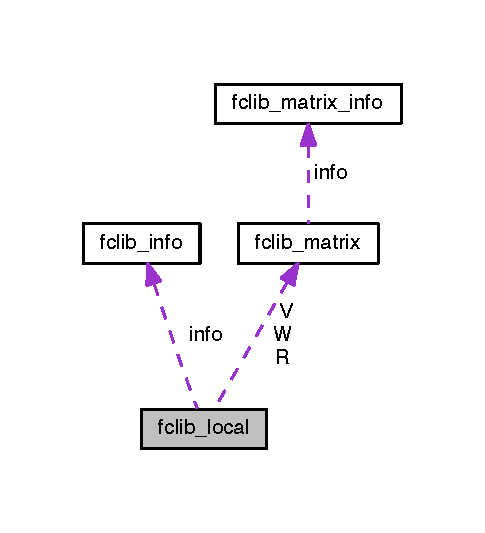
\includegraphics[width=233pt]{structfclib__local__coll__graph}
\end{center}
\end{figure}
\subsubsection*{Public Attributes}
\begin{DoxyCompactItemize}
\item 
struct \hyperlink{structfclib__matrix}{fclib\+\_\+matrix} $\ast$ \hyperlink{structfclib__local_a981b5abb9acf3f99dffe9a05602ad864}{W}
\begin{DoxyCompactList}\small\item\em the matrix W (see mathematical description below) \end{DoxyCompactList}\item 
struct \hyperlink{structfclib__matrix}{fclib\+\_\+matrix} $\ast$ \hyperlink{structfclib__local_a516663ee92260f82283b4933f7e098cf}{V}
\begin{DoxyCompactList}\small\item\em the matrix V (see mathematical description below) \end{DoxyCompactList}\item 
struct \hyperlink{structfclib__matrix}{fclib\+\_\+matrix} $\ast$ \hyperlink{structfclib__local_ae08751b33a0771d54d48aee48f838ced}{R}
\begin{DoxyCompactList}\small\item\em the matrix R (see mathematical description below) \end{DoxyCompactList}\item 
double $\ast$ \hyperlink{structfclib__local_a90d9490cac0bc9b69fd13253882f1557}{mu}
\begin{DoxyCompactList}\small\item\em the vector $\mu$ of coefficient of friction (see mathematical description below) \end{DoxyCompactList}\item 
double $\ast$ \hyperlink{structfclib__local_a9a032092a828a13a7e106cce4ba7ad96}{q}
\begin{DoxyCompactList}\small\item\em the vector q (see mathematical description below) \end{DoxyCompactList}\item 
double $\ast$ \hyperlink{structfclib__local_abb6b3a07d92a86aac1c38e4d847207e3}{s}
\begin{DoxyCompactList}\small\item\em the vector s (see mathematical description below) \end{DoxyCompactList}\item 
int \hyperlink{structfclib__local_accf07018913652e57be3a661b25d8bb7}{spacedim}
\begin{DoxyCompactList}\small\item\em the dimension , 2 or 3, of the local space at contact (2d or 3d friction contact laws) \end{DoxyCompactList}\item 
struct \hyperlink{structfclib__info}{fclib\+\_\+info} $\ast$ \hyperlink{structfclib__local_ababce9da71cdb99e4928a596dde8bc89}{info}
\begin{DoxyCompactList}\small\item\em info on the problem \end{DoxyCompactList}\end{DoxyCompactItemize}


\subsubsection{Detailed Description}
The local frictional contact problem defined by. 

given 
\begin{DoxyItemize}
\item a positive semi--definite matrix ${W} \in {\mathrm{I\!R}}^{m \times m}$ 
\item a matrix ${V} \in {\mathrm{I\!R}}^{m \times p}$ 
\item a matrix ${R} \in {\mathrm{I\!R}}^{p \times p}$ 
\item a vector $q \in {\mathrm{I\!R}}^{m}$, 
\item a vector $s \in {\mathrm{I\!R}}^{p}$, 
\item a vector of coefficients of friction $\mu \in {\mathrm{I\!R}}^{n_c}$ 
\end{DoxyItemize}the Mixed 3\+D\+F\+C problem is to find three vectors $u\in{\mathrm{I\!R}}^m$, $r\in {\mathrm{I\!R}}^m$ and $\lambda \in {\mathrm{I\!R}}^p$ denoted by $\mathrm{M3DFC}(R,V,W,q,s,\mu)$ such that \begin{eqnarray*}\label{eq:lcp1} *\begin{cases} V^T {r} + R \lambda + s = 0 \\ \ \ \hat u = W {r} + V\lambda + q +\left[ \left[\begin{array}{c} \mu^\alpha \|u^\alpha_T\|\ \ 0 \ \ 0 \end{array}\right]^T, \alpha = 1 \ldots n_c \right]^T \\ \ \ C^\star_{\mu} \ni {\hat u} \perp r \in C_{\mu} \end{cases} \end{eqnarray*} where the Coulomb friction cone for a contact $\alpha$ is defined by \begin{eqnarray*} \label{eq:CCC} C_{\mu^\alpha}^{\alpha} = \{r^\alpha, \|r^\alpha_T \| \leq \mu^\alpha |r^\alpha_N| \} \end{eqnarray*} and the set $C^{\alpha,\star}_{\mu^\alpha}$ is its dual. 

Definition at line 228 of file fclib.\+h.



\subsubsection{Member Data Documentation}
\hypertarget{structfclib__local_a981b5abb9acf3f99dffe9a05602ad864}{}\index{fclib\+\_\+local@{fclib\+\_\+local}!W@{W}}
\index{W@{W}!fclib\+\_\+local@{fclib\+\_\+local}}
\paragraph[{W}]{\setlength{\rightskip}{0pt plus 5cm}struct {\bf fclib\+\_\+matrix}$\ast$ fclib\+\_\+local\+::\+W}\label{structfclib__local_a981b5abb9acf3f99dffe9a05602ad864}


the matrix W (see mathematical description below) 



Definition at line 231 of file fclib.\+h.



Referenced by compare\+\_\+local\+\_\+problems(), fclib\+\_\+delete\+\_\+local(), fclib\+\_\+merit\+\_\+local(), fclib\+\_\+read\+\_\+local(), fclib\+\_\+write\+\_\+local(), main(), random\+\_\+local\+\_\+problem(), random\+\_\+local\+\_\+solutions(), read\+\_\+local\+\_\+vectors(), and write\+\_\+local\+\_\+vectors().

\hypertarget{structfclib__local_a516663ee92260f82283b4933f7e098cf}{}\index{fclib\+\_\+local@{fclib\+\_\+local}!V@{V}}
\index{V@{V}!fclib\+\_\+local@{fclib\+\_\+local}}
\paragraph[{V}]{\setlength{\rightskip}{0pt plus 5cm}struct {\bf fclib\+\_\+matrix}$\ast$ fclib\+\_\+local\+::\+V}\label{structfclib__local_a516663ee92260f82283b4933f7e098cf}


the matrix V (see mathematical description below) 



Definition at line 233 of file fclib.\+h.



Referenced by compare\+\_\+local\+\_\+problems(), fclib\+\_\+delete\+\_\+local(), fclib\+\_\+merit\+\_\+local(), fclib\+\_\+read\+\_\+local(), fclib\+\_\+write\+\_\+local(), random\+\_\+local\+\_\+problem(), and write\+\_\+local\+\_\+vectors().

\hypertarget{structfclib__local_ae08751b33a0771d54d48aee48f838ced}{}\index{fclib\+\_\+local@{fclib\+\_\+local}!R@{R}}
\index{R@{R}!fclib\+\_\+local@{fclib\+\_\+local}}
\paragraph[{R}]{\setlength{\rightskip}{0pt plus 5cm}struct {\bf fclib\+\_\+matrix}$\ast$ fclib\+\_\+local\+::\+R}\label{structfclib__local_ae08751b33a0771d54d48aee48f838ced}


the matrix R (see mathematical description below) 



Definition at line 235 of file fclib.\+h.



Referenced by compare\+\_\+local\+\_\+problems(), fclib\+\_\+delete\+\_\+local(), fclib\+\_\+merit\+\_\+local(), fclib\+\_\+read\+\_\+local(), fclib\+\_\+write\+\_\+local(), main(), random\+\_\+local\+\_\+problem(), random\+\_\+local\+\_\+solutions(), read\+\_\+local\+\_\+vectors(), and write\+\_\+local\+\_\+vectors().

\hypertarget{structfclib__local_a90d9490cac0bc9b69fd13253882f1557}{}\index{fclib\+\_\+local@{fclib\+\_\+local}!mu@{mu}}
\index{mu@{mu}!fclib\+\_\+local@{fclib\+\_\+local}}
\paragraph[{mu}]{\setlength{\rightskip}{0pt plus 5cm}double$\ast$ fclib\+\_\+local\+::mu}\label{structfclib__local_a90d9490cac0bc9b69fd13253882f1557}


the vector $\mu$ of coefficient of friction (see mathematical description below) 



Definition at line 237 of file fclib.\+h.



Referenced by compare\+\_\+local\+\_\+problems(), fclib\+\_\+delete\+\_\+local(), fclib\+\_\+merit\+\_\+local(), random\+\_\+local\+\_\+problem(), read\+\_\+local\+\_\+vectors(), and write\+\_\+local\+\_\+vectors().

\hypertarget{structfclib__local_a9a032092a828a13a7e106cce4ba7ad96}{}\index{fclib\+\_\+local@{fclib\+\_\+local}!q@{q}}
\index{q@{q}!fclib\+\_\+local@{fclib\+\_\+local}}
\paragraph[{q}]{\setlength{\rightskip}{0pt plus 5cm}double$\ast$ fclib\+\_\+local\+::q}\label{structfclib__local_a9a032092a828a13a7e106cce4ba7ad96}


the vector q (see mathematical description below) 



Definition at line 239 of file fclib.\+h.



Referenced by compare\+\_\+local\+\_\+problems(), fclib\+\_\+delete\+\_\+local(), fclib\+\_\+merit\+\_\+local(), random\+\_\+local\+\_\+problem(), read\+\_\+local\+\_\+vectors(), and write\+\_\+local\+\_\+vectors().

\hypertarget{structfclib__local_abb6b3a07d92a86aac1c38e4d847207e3}{}\index{fclib\+\_\+local@{fclib\+\_\+local}!s@{s}}
\index{s@{s}!fclib\+\_\+local@{fclib\+\_\+local}}
\paragraph[{s}]{\setlength{\rightskip}{0pt plus 5cm}double$\ast$ fclib\+\_\+local\+::s}\label{structfclib__local_abb6b3a07d92a86aac1c38e4d847207e3}


the vector s (see mathematical description below) 



Definition at line 241 of file fclib.\+h.



Referenced by compare\+\_\+local\+\_\+problems(), fclib\+\_\+delete\+\_\+local(), fclib\+\_\+merit\+\_\+local(), random\+\_\+local\+\_\+problem(), read\+\_\+local\+\_\+vectors(), and write\+\_\+local\+\_\+vectors().

\hypertarget{structfclib__local_accf07018913652e57be3a661b25d8bb7}{}\index{fclib\+\_\+local@{fclib\+\_\+local}!spacedim@{spacedim}}
\index{spacedim@{spacedim}!fclib\+\_\+local@{fclib\+\_\+local}}
\paragraph[{spacedim}]{\setlength{\rightskip}{0pt plus 5cm}int fclib\+\_\+local\+::spacedim}\label{structfclib__local_accf07018913652e57be3a661b25d8bb7}


the dimension , 2 or 3, of the local space at contact (2d or 3d friction contact laws) 



Definition at line 243 of file fclib.\+h.



Referenced by compare\+\_\+local\+\_\+problems(), fclib\+\_\+merit\+\_\+local(), fclib\+\_\+read\+\_\+local(), fclib\+\_\+write\+\_\+local(), random\+\_\+local\+\_\+problem(), read\+\_\+local\+\_\+vectors(), and write\+\_\+local\+\_\+vectors().

\hypertarget{structfclib__local_ababce9da71cdb99e4928a596dde8bc89}{}\index{fclib\+\_\+local@{fclib\+\_\+local}!info@{info}}
\index{info@{info}!fclib\+\_\+local@{fclib\+\_\+local}}
\paragraph[{info}]{\setlength{\rightskip}{0pt plus 5cm}struct {\bf fclib\+\_\+info}$\ast$ fclib\+\_\+local\+::info}\label{structfclib__local_ababce9da71cdb99e4928a596dde8bc89}


info on the problem 



Definition at line 245 of file fclib.\+h.



Referenced by compare\+\_\+local\+\_\+problems(), fclib\+\_\+delete\+\_\+local(), fclib\+\_\+read\+\_\+local(), fclib\+\_\+write\+\_\+local(), and random\+\_\+local\+\_\+problem().


\hypertarget{structfclib__matrix}{}\subsection{fclib\+\_\+matrix Struct Reference}
\label{structfclib__matrix}\index{fclib\+\_\+matrix@{fclib\+\_\+matrix}}


matrix in compressed row/column or triplet form  




{\ttfamily \#include $<$fclib.\+h$>$}



Collaboration diagram for fclib\+\_\+matrix\+:
\nopagebreak
\begin{figure}[H]
\begin{center}
\leavevmode
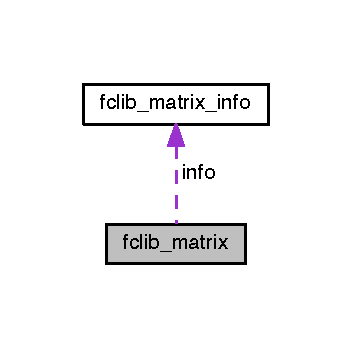
\includegraphics[width=169pt]{structfclib__matrix__coll__graph}
\end{center}
\end{figure}
\subsubsection*{Public Attributes}
\begin{DoxyCompactItemize}
\item 
int \hyperlink{structfclib__matrix_ad59323011143dc70ef74f4377279e0d0}{nzmax}
\begin{DoxyCompactList}\small\item\em maximum number of entries \end{DoxyCompactList}\item 
int \hyperlink{structfclib__matrix_aaec2a835fcc339c3fb84227e2f7b861b}{m}
\begin{DoxyCompactList}\small\item\em number of rows \end{DoxyCompactList}\item 
int \hyperlink{structfclib__matrix_ace0c395ca5da8a4bcc4958a29895c639}{n}
\begin{DoxyCompactList}\small\item\em number of columns \end{DoxyCompactList}\item 
int $\ast$ \hyperlink{structfclib__matrix_ace167d937e3c1bb2558e264aefada841}{p}
\begin{DoxyCompactList}\small\item\em compressed\+: row (size m+1) or column (size n+1) pointers; triplet\+: row indices (size nz) \end{DoxyCompactList}\item 
int $\ast$ \hyperlink{structfclib__matrix_aed86c681657206e7502450e437dba667}{i}
\begin{DoxyCompactList}\small\item\em compressed\+: column or row indices, size nzmax; triplet\+: column indices (size nz) \end{DoxyCompactList}\item 
double $\ast$ \hyperlink{structfclib__matrix_aba1891f51a81f973249456c91715e06d}{x}
\begin{DoxyCompactList}\small\item\em numerical values, size nzmax \end{DoxyCompactList}\item 
int \hyperlink{structfclib__matrix_a7d64a7cddc93a8e1f96ab32e9afe0bbb}{nz}
\begin{DoxyCompactList}\small\item\em \subsubsection*{of entries in triplet matrix, -\/1 for compressed columns, -\/2 for compressed rows}\end{DoxyCompactList}\item 
struct \hyperlink{structfclib__matrix__info}{fclib\+\_\+matrix\+\_\+info} $\ast$ \hyperlink{structfclib__matrix_ac0af227334c5b0a13a3222c8f04add36}{info}
\begin{DoxyCompactList}\small\item\em info for this matrix \end{DoxyCompactList}\end{DoxyCompactItemize}


\subsubsection{Detailed Description}
matrix in compressed row/column or triplet form 

Definition at line 119 of file fclib.\+h.



\subsubsection{Member Data Documentation}
\hypertarget{structfclib__matrix_ad59323011143dc70ef74f4377279e0d0}{}\index{fclib\+\_\+matrix@{fclib\+\_\+matrix}!nzmax@{nzmax}}
\index{nzmax@{nzmax}!fclib\+\_\+matrix@{fclib\+\_\+matrix}}
\paragraph[{nzmax}]{\setlength{\rightskip}{0pt plus 5cm}int fclib\+\_\+matrix\+::nzmax}\label{structfclib__matrix_ad59323011143dc70ef74f4377279e0d0}


maximum number of entries 



Definition at line 122 of file fclib.\+h.



Referenced by compare\+\_\+matrices(), random\+\_\+matrix(), read\+\_\+matrix(), and write\+\_\+matrix().

\hypertarget{structfclib__matrix_aaec2a835fcc339c3fb84227e2f7b861b}{}\index{fclib\+\_\+matrix@{fclib\+\_\+matrix}!m@{m}}
\index{m@{m}!fclib\+\_\+matrix@{fclib\+\_\+matrix}}
\paragraph[{m}]{\setlength{\rightskip}{0pt plus 5cm}int fclib\+\_\+matrix\+::m}\label{structfclib__matrix_aaec2a835fcc339c3fb84227e2f7b861b}


number of rows 



Definition at line 124 of file fclib.\+h.



Referenced by compare\+\_\+global\+\_\+problems(), compare\+\_\+matrices(), main(), matrix\+\_\+info(), random\+\_\+matrix(), read\+\_\+global\+\_\+vectors(), read\+\_\+local\+\_\+vectors(), read\+\_\+matrix(), write\+\_\+global\+\_\+vectors(), write\+\_\+local\+\_\+vectors(), and write\+\_\+matrix().

\hypertarget{structfclib__matrix_ace0c395ca5da8a4bcc4958a29895c639}{}\index{fclib\+\_\+matrix@{fclib\+\_\+matrix}!n@{n}}
\index{n@{n}!fclib\+\_\+matrix@{fclib\+\_\+matrix}}
\paragraph[{n}]{\setlength{\rightskip}{0pt plus 5cm}int fclib\+\_\+matrix\+::n}\label{structfclib__matrix_ace0c395ca5da8a4bcc4958a29895c639}


number of columns 



Definition at line 126 of file fclib.\+h.



Referenced by compare\+\_\+global\+\_\+problems(), compare\+\_\+local\+\_\+problems(), compare\+\_\+matrices(), fclib\+\_\+merit\+\_\+local(), main(), random\+\_\+global\+\_\+problem(), random\+\_\+global\+\_\+solutions(), random\+\_\+local\+\_\+solutions(), random\+\_\+matrix(), read\+\_\+global\+\_\+vectors(), read\+\_\+matrix(), write\+\_\+global\+\_\+vectors(), and write\+\_\+matrix().

\hypertarget{structfclib__matrix_ace167d937e3c1bb2558e264aefada841}{}\index{fclib\+\_\+matrix@{fclib\+\_\+matrix}!p@{p}}
\index{p@{p}!fclib\+\_\+matrix@{fclib\+\_\+matrix}}
\paragraph[{p}]{\setlength{\rightskip}{0pt plus 5cm}int$\ast$ fclib\+\_\+matrix\+::p}\label{structfclib__matrix_ace167d937e3c1bb2558e264aefada841}


compressed\+: row (size m+1) or column (size n+1) pointers; triplet\+: row indices (size nz) 



Definition at line 128 of file fclib.\+h.



Referenced by compare\+\_\+matrices(), delete\+\_\+matrix(), random\+\_\+matrix(), read\+\_\+matrix(), and write\+\_\+matrix().

\hypertarget{structfclib__matrix_aed86c681657206e7502450e437dba667}{}\index{fclib\+\_\+matrix@{fclib\+\_\+matrix}!i@{i}}
\index{i@{i}!fclib\+\_\+matrix@{fclib\+\_\+matrix}}
\paragraph[{i}]{\setlength{\rightskip}{0pt plus 5cm}int$\ast$ fclib\+\_\+matrix\+::i}\label{structfclib__matrix_aed86c681657206e7502450e437dba667}


compressed\+: column or row indices, size nzmax; triplet\+: column indices (size nz) 



Definition at line 130 of file fclib.\+h.



Referenced by compare\+\_\+matrices(), delete\+\_\+matrix(), fclib\+\_\+merit\+\_\+local(), random\+\_\+matrix(), read\+\_\+matrix(), and write\+\_\+matrix().

\hypertarget{structfclib__matrix_aba1891f51a81f973249456c91715e06d}{}\index{fclib\+\_\+matrix@{fclib\+\_\+matrix}!x@{x}}
\index{x@{x}!fclib\+\_\+matrix@{fclib\+\_\+matrix}}
\paragraph[{x}]{\setlength{\rightskip}{0pt plus 5cm}double$\ast$ fclib\+\_\+matrix\+::x}\label{structfclib__matrix_aba1891f51a81f973249456c91715e06d}


numerical values, size nzmax 



Definition at line 132 of file fclib.\+h.



Referenced by compare\+\_\+matrices(), delete\+\_\+matrix(), random\+\_\+matrix(), read\+\_\+matrix(), and write\+\_\+matrix().

\hypertarget{structfclib__matrix_a7d64a7cddc93a8e1f96ab32e9afe0bbb}{}\index{fclib\+\_\+matrix@{fclib\+\_\+matrix}!nz@{nz}}
\index{nz@{nz}!fclib\+\_\+matrix@{fclib\+\_\+matrix}}
\paragraph[{nz}]{\setlength{\rightskip}{0pt plus 5cm}int fclib\+\_\+matrix\+::nz}\label{structfclib__matrix_a7d64a7cddc93a8e1f96ab32e9afe0bbb}


\subsubsection*{of entries in triplet matrix, -\/1 for compressed columns, -\/2 for compressed rows}



Definition at line 134 of file fclib.\+h.



Referenced by compare\+\_\+matrices(), random\+\_\+matrix(), read\+\_\+matrix(), and write\+\_\+matrix().

\hypertarget{structfclib__matrix_ac0af227334c5b0a13a3222c8f04add36}{}\index{fclib\+\_\+matrix@{fclib\+\_\+matrix}!info@{info}}
\index{info@{info}!fclib\+\_\+matrix@{fclib\+\_\+matrix}}
\paragraph[{info}]{\setlength{\rightskip}{0pt plus 5cm}struct {\bf fclib\+\_\+matrix\+\_\+info}$\ast$ fclib\+\_\+matrix\+::info}\label{structfclib__matrix_ac0af227334c5b0a13a3222c8f04add36}


info for this matrix 



Definition at line 136 of file fclib.\+h.



Referenced by compare\+\_\+matrices(), delete\+\_\+matrix(), random\+\_\+matrix(), read\+\_\+matrix(), and write\+\_\+matrix().


\hypertarget{structfclib__matrix__info}{}\subsection{fclib\+\_\+matrix\+\_\+info Struct Reference}
\label{structfclib__matrix__info}\index{fclib\+\_\+matrix\+\_\+info@{fclib\+\_\+matrix\+\_\+info}}


This structure allows the user to enter a description for a given matrix (comment, conditionning, determinant, rank.) if they are known.  




{\ttfamily \#include $<$fclib.\+h$>$}

\subsubsection*{Public Attributes}
\begin{DoxyCompactItemize}
\item 
char $\ast$ \hyperlink{structfclib__matrix__info_a9c4994b1759bf3a7a75c72cd78709722}{comment}
\begin{DoxyCompactList}\small\item\em comment on the matrix properties \end{DoxyCompactList}\item 
double \hyperlink{structfclib__matrix__info_a453db794429411025f2b8dfb497f5f35}{conditioning}
\begin{DoxyCompactList}\small\item\em conditioning \end{DoxyCompactList}\item 
double \hyperlink{structfclib__matrix__info_a9c6697aee458be4494b215f0f003ca48}{determinant}
\begin{DoxyCompactList}\small\item\em determinant \end{DoxyCompactList}\item 
int \hyperlink{structfclib__matrix__info_af838043a1769956958c4a66e6227227d}{rank}
\begin{DoxyCompactList}\small\item\em rank \end{DoxyCompactList}\end{DoxyCompactItemize}


\subsubsection{Detailed Description}
This structure allows the user to enter a description for a given matrix (comment, conditionning, determinant, rank.) if they are known. 

Definition at line 105 of file fclib.\+h.



\subsubsection{Member Data Documentation}
\hypertarget{structfclib__matrix__info_a9c4994b1759bf3a7a75c72cd78709722}{}\index{fclib\+\_\+matrix\+\_\+info@{fclib\+\_\+matrix\+\_\+info}!comment@{comment}}
\index{comment@{comment}!fclib\+\_\+matrix\+\_\+info@{fclib\+\_\+matrix\+\_\+info}}
\paragraph[{comment}]{\setlength{\rightskip}{0pt plus 5cm}char$\ast$ fclib\+\_\+matrix\+\_\+info\+::comment}\label{structfclib__matrix__info_a9c4994b1759bf3a7a75c72cd78709722}


comment on the matrix properties 



Definition at line 108 of file fclib.\+h.



Referenced by compare\+\_\+matrix\+\_\+infos(), delete\+\_\+matrix\+\_\+info(), matrix\+\_\+info(), read\+\_\+matrix(), and write\+\_\+matrix().

\hypertarget{structfclib__matrix__info_a453db794429411025f2b8dfb497f5f35}{}\index{fclib\+\_\+matrix\+\_\+info@{fclib\+\_\+matrix\+\_\+info}!conditioning@{conditioning}}
\index{conditioning@{conditioning}!fclib\+\_\+matrix\+\_\+info@{fclib\+\_\+matrix\+\_\+info}}
\paragraph[{conditioning}]{\setlength{\rightskip}{0pt plus 5cm}double fclib\+\_\+matrix\+\_\+info\+::conditioning}\label{structfclib__matrix__info_a453db794429411025f2b8dfb497f5f35}


conditioning 



Definition at line 110 of file fclib.\+h.



Referenced by compare\+\_\+matrix\+\_\+infos(), matrix\+\_\+info(), read\+\_\+matrix(), and write\+\_\+matrix().

\hypertarget{structfclib__matrix__info_a9c6697aee458be4494b215f0f003ca48}{}\index{fclib\+\_\+matrix\+\_\+info@{fclib\+\_\+matrix\+\_\+info}!determinant@{determinant}}
\index{determinant@{determinant}!fclib\+\_\+matrix\+\_\+info@{fclib\+\_\+matrix\+\_\+info}}
\paragraph[{determinant}]{\setlength{\rightskip}{0pt plus 5cm}double fclib\+\_\+matrix\+\_\+info\+::determinant}\label{structfclib__matrix__info_a9c6697aee458be4494b215f0f003ca48}


determinant 



Definition at line 112 of file fclib.\+h.



Referenced by compare\+\_\+matrix\+\_\+infos(), matrix\+\_\+info(), read\+\_\+matrix(), and write\+\_\+matrix().

\hypertarget{structfclib__matrix__info_af838043a1769956958c4a66e6227227d}{}\index{fclib\+\_\+matrix\+\_\+info@{fclib\+\_\+matrix\+\_\+info}!rank@{rank}}
\index{rank@{rank}!fclib\+\_\+matrix\+\_\+info@{fclib\+\_\+matrix\+\_\+info}}
\paragraph[{rank}]{\setlength{\rightskip}{0pt plus 5cm}int fclib\+\_\+matrix\+\_\+info\+::rank}\label{structfclib__matrix__info_af838043a1769956958c4a66e6227227d}


rank 



Definition at line 114 of file fclib.\+h.



Referenced by compare\+\_\+matrix\+\_\+infos(), matrix\+\_\+info(), read\+\_\+matrix(), and write\+\_\+matrix().


\hypertarget{structfclib__solution}{}\subsection{fclib\+\_\+solution Struct Reference}
\label{structfclib__solution}\index{fclib\+\_\+solution@{fclib\+\_\+solution}}


A solution or a guess for the frictional contact problem.  




{\ttfamily \#include $<$fclib.\+h$>$}

\subsubsection*{Public Attributes}
\begin{DoxyCompactItemize}
\item 
double $\ast$ \hyperlink{structfclib__solution_a252982ce524686a094223a55c194fea8}{v}
\begin{DoxyCompactList}\small\item\em global velocity (or position/displacement for quasi-\/static problems) solution vector \end{DoxyCompactList}\item 
double $\ast$ \hyperlink{structfclib__solution_acb160f0dad04b9420388464d256ae41f}{u}
\begin{DoxyCompactList}\small\item\em local velocity (or position/displacement for quasi-\/static problems) solution vector \end{DoxyCompactList}\item 
double $\ast$ \hyperlink{structfclib__solution_aba0437aebbb1060350ef2f0a6e8b504d}{r}
\begin{DoxyCompactList}\small\item\em local contact forces (or impulses) solution vector \end{DoxyCompactList}\item 
double $\ast$ \hyperlink{structfclib__solution_a872a687856540dd19286aec43d890ede}{l}
\begin{DoxyCompactList}\small\item\em multiplier for equlity constraints ( $\lambda$) solution vector \end{DoxyCompactList}\end{DoxyCompactItemize}


\subsubsection{Detailed Description}
A solution or a guess for the frictional contact problem. 

This structure allows to store a solution vector of a guess vector for the various frictional contact problems. 

Definition at line 255 of file fclib.\+h.



\subsubsection{Member Data Documentation}
\hypertarget{structfclib__solution_a252982ce524686a094223a55c194fea8}{}\index{fclib\+\_\+solution@{fclib\+\_\+solution}!v@{v}}
\index{v@{v}!fclib\+\_\+solution@{fclib\+\_\+solution}}
\paragraph[{v}]{\setlength{\rightskip}{0pt plus 5cm}double$\ast$ fclib\+\_\+solution\+::v}\label{structfclib__solution_a252982ce524686a094223a55c194fea8}


global velocity (or position/displacement for quasi-\/static problems) solution vector 



Definition at line 258 of file fclib.\+h.



Referenced by compare\+\_\+solutions(), fclib\+\_\+delete\+\_\+solutions(), fclib\+\_\+merit\+\_\+local(), random\+\_\+global\+\_\+solutions(), random\+\_\+local\+\_\+solutions(), read\+\_\+solution(), and write\+\_\+solution().

\hypertarget{structfclib__solution_acb160f0dad04b9420388464d256ae41f}{}\index{fclib\+\_\+solution@{fclib\+\_\+solution}!u@{u}}
\index{u@{u}!fclib\+\_\+solution@{fclib\+\_\+solution}}
\paragraph[{u}]{\setlength{\rightskip}{0pt plus 5cm}double$\ast$ fclib\+\_\+solution\+::u}\label{structfclib__solution_acb160f0dad04b9420388464d256ae41f}


local velocity (or position/displacement for quasi-\/static problems) solution vector 



Definition at line 260 of file fclib.\+h.



Referenced by compare\+\_\+solutions(), fclib\+\_\+delete\+\_\+solutions(), fclib\+\_\+merit\+\_\+local(), random\+\_\+global\+\_\+solutions(), random\+\_\+local\+\_\+solutions(), read\+\_\+solution(), and write\+\_\+solution().

\hypertarget{structfclib__solution_aba0437aebbb1060350ef2f0a6e8b504d}{}\index{fclib\+\_\+solution@{fclib\+\_\+solution}!r@{r}}
\index{r@{r}!fclib\+\_\+solution@{fclib\+\_\+solution}}
\paragraph[{r}]{\setlength{\rightskip}{0pt plus 5cm}double$\ast$ fclib\+\_\+solution\+::r}\label{structfclib__solution_aba0437aebbb1060350ef2f0a6e8b504d}


local contact forces (or impulses) solution vector 



Definition at line 262 of file fclib.\+h.



Referenced by compare\+\_\+solutions(), fclib\+\_\+delete\+\_\+solutions(), fclib\+\_\+merit\+\_\+local(), random\+\_\+global\+\_\+solutions(), random\+\_\+local\+\_\+solutions(), read\+\_\+solution(), and write\+\_\+solution().

\hypertarget{structfclib__solution_a872a687856540dd19286aec43d890ede}{}\index{fclib\+\_\+solution@{fclib\+\_\+solution}!l@{l}}
\index{l@{l}!fclib\+\_\+solution@{fclib\+\_\+solution}}
\paragraph[{l}]{\setlength{\rightskip}{0pt plus 5cm}double$\ast$ fclib\+\_\+solution\+::l}\label{structfclib__solution_a872a687856540dd19286aec43d890ede}


multiplier for equlity constraints ( $\lambda$) solution vector 



Definition at line 264 of file fclib.\+h.



Referenced by compare\+\_\+solutions(), fclib\+\_\+delete\+\_\+solutions(), fclib\+\_\+merit\+\_\+local(), random\+\_\+global\+\_\+solutions(), random\+\_\+local\+\_\+solutions(), read\+\_\+solution(), and write\+\_\+solution().


\section{File Documentation}
\hypertarget{additionalpages_8doxygen}{}\subsection{additionalpages.\+doxygen File Reference}
\label{additionalpages_8doxygen}\index{additionalpages.\+doxygen@{additionalpages.\+doxygen}}

\hypertarget{fcint_8h}{}\subsection{fcint.\+h File Reference}
\label{fcint_8h}\index{fcint.\+h@{fcint.\+h}}
This graph shows which files directly or indirectly include this file\+:\nopagebreak
\begin{figure}[H]
\begin{center}
\leavevmode
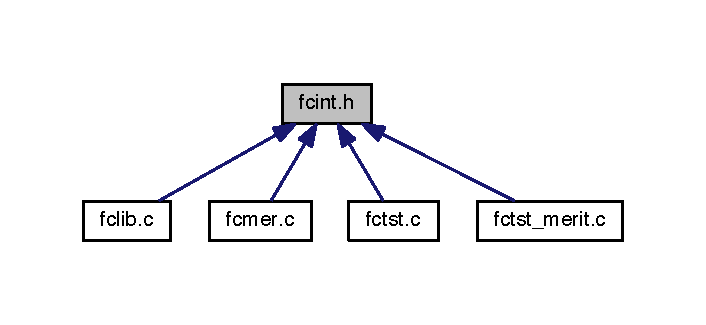
\includegraphics[width=339pt]{fcint_8h__dep__incl}
\end{center}
\end{figure}
\subsubsection*{Macros}
\begin{DoxyCompactItemize}
\item 
\#define \hyperlink{fcint_8h_af6a170071ba1da3930abadc6d3f95493}{A\+S\+S\+E\+R\+T}(Test, ...)
\item 
\#define \hyperlink{fcint_8h_a7e1b7988c998844258179660bb5f8e69}{I\+O}(Call)~\hyperlink{fcint_8h_af6a170071ba1da3930abadc6d3f95493}{A\+S\+S\+E\+R\+T} ((Call) $>$= 0, \char`\"{}E\+R\+R\+O\+R\+: H\+D\+F5 call failed\char`\"{})
\item 
\#define \hyperlink{fcint_8h_ae5d192dca25b682622b72b1211df96b7}{M\+M}(Call)~\hyperlink{fcint_8h_af6a170071ba1da3930abadc6d3f95493}{A\+S\+S\+E\+R\+T} ((Call), \char`\"{}E\+R\+R\+O\+R\+: out of memory\char`\"{})
\end{DoxyCompactItemize}


\subsubsection{Macro Definition Documentation}
\hypertarget{fcint_8h_af6a170071ba1da3930abadc6d3f95493}{}\index{fcint.\+h@{fcint.\+h}!A\+S\+S\+E\+R\+T@{A\+S\+S\+E\+R\+T}}
\index{A\+S\+S\+E\+R\+T@{A\+S\+S\+E\+R\+T}!fcint.\+h@{fcint.\+h}}
\paragraph[{A\+S\+S\+E\+R\+T}]{\setlength{\rightskip}{0pt plus 5cm}\#define A\+S\+S\+E\+R\+T(
\begin{DoxyParamCaption}
\item[{}]{Test, }
\item[{}]{...}
\end{DoxyParamCaption}
)}\label{fcint_8h_af6a170071ba1da3930abadc6d3f95493}
{\bfseries Value\+:}
\begin{DoxyCode}
\textcolor{keywordflow}{do} \{\(\backslash\)
  if (! (Test)) \{ fprintf (stderr, \textcolor{stringliteral}{"%s: %d => "}, \_\_FILE\_\_, \_\_LINE\_\_);\(\backslash\)
    fprintf (stderr, \_\_VA\_ARGS\_\_);\(\backslash\)
    fprintf (stderr, \textcolor{stringliteral}{"\(\backslash\)n"}); exit (1); \} \} \textcolor{keywordflow}{while} (0)
\end{DoxyCode}


Definition at line 29 of file fcint.\+h.



Referenced by fclib\+\_\+write\+\_\+global(), fclib\+\_\+write\+\_\+local(), main(), read\+\_\+global\+\_\+vectors(), read\+\_\+local\+\_\+vectors(), read\+\_\+matrix(), read\+\_\+solution(), write\+\_\+global\+\_\+vectors(), write\+\_\+local\+\_\+vectors(), write\+\_\+matrix(), and write\+\_\+solution().

\hypertarget{fcint_8h_a7e1b7988c998844258179660bb5f8e69}{}\index{fcint.\+h@{fcint.\+h}!I\+O@{I\+O}}
\index{I\+O@{I\+O}!fcint.\+h@{fcint.\+h}}
\paragraph[{I\+O}]{\setlength{\rightskip}{0pt plus 5cm}\#define I\+O(
\begin{DoxyParamCaption}
\item[{}]{Call}
\end{DoxyParamCaption}
)~{\bf A\+S\+S\+E\+R\+T} ((Call) $>$= 0, \char`\"{}E\+R\+R\+O\+R\+: H\+D\+F5 call failed\char`\"{})}\label{fcint_8h_a7e1b7988c998844258179660bb5f8e69}


Definition at line 35 of file fcint.\+h.



Referenced by fclib\+\_\+create\+\_\+int\+\_\+attributes\+\_\+in\+\_\+info(), fclib\+\_\+read\+\_\+global(), fclib\+\_\+read\+\_\+guesses(), fclib\+\_\+read\+\_\+local(), fclib\+\_\+read\+\_\+solution(), fclib\+\_\+write\+\_\+global(), fclib\+\_\+write\+\_\+guesses(), fclib\+\_\+write\+\_\+local(), fclib\+\_\+write\+\_\+solution(), read\+\_\+global\+\_\+vectors(), read\+\_\+local\+\_\+vectors(), read\+\_\+matrix(), read\+\_\+nvnunrnl(), read\+\_\+problem\+\_\+info(), read\+\_\+solution(), write\+\_\+global\+\_\+vectors(), write\+\_\+local\+\_\+vectors(), write\+\_\+matrix(), write\+\_\+problem\+\_\+info(), and write\+\_\+solution().

\hypertarget{fcint_8h_ae5d192dca25b682622b72b1211df96b7}{}\index{fcint.\+h@{fcint.\+h}!M\+M@{M\+M}}
\index{M\+M@{M\+M}!fcint.\+h@{fcint.\+h}}
\paragraph[{M\+M}]{\setlength{\rightskip}{0pt plus 5cm}\#define M\+M(
\begin{DoxyParamCaption}
\item[{}]{Call}
\end{DoxyParamCaption}
)~{\bf A\+S\+S\+E\+R\+T} ((Call), \char`\"{}E\+R\+R\+O\+R\+: out of memory\char`\"{})}\label{fcint_8h_ae5d192dca25b682622b72b1211df96b7}


Definition at line 36 of file fcint.\+h.



Referenced by fclib\+\_\+read\+\_\+global(), fclib\+\_\+read\+\_\+guesses(), fclib\+\_\+read\+\_\+local(), fclib\+\_\+read\+\_\+solution(), matrix\+\_\+info(), problem\+\_\+info(), random\+\_\+global\+\_\+problem(), random\+\_\+global\+\_\+solutions(), random\+\_\+local\+\_\+problem(), random\+\_\+local\+\_\+solutions(), random\+\_\+matrix(), random\+\_\+vector(), read\+\_\+global\+\_\+vectors(), read\+\_\+local\+\_\+vectors(), read\+\_\+matrix(), read\+\_\+problem\+\_\+info(), and read\+\_\+solution().


\hypertarget{fclib_8c}{}\subsection{fclib.\+c File Reference}
\label{fclib_8c}\index{fclib.\+c@{fclib.\+c}}
{\ttfamily \#include $<$string.\+h$>$}\\*
{\ttfamily \#include $<$stdlib.\+h$>$}\\*
{\ttfamily \#include $<$stdio.\+h$>$}\\*
{\ttfamily \#include $<$hdf5.\+h$>$}\\*
{\ttfamily \#include $<$hdf5\+\_\+hl.\+h$>$}\\*
{\ttfamily \#include \char`\"{}fclib.\+h\char`\"{}}\\*
{\ttfamily \#include \char`\"{}fcint.\+h\char`\"{}}\\*
Include dependency graph for fclib.\+c\+:\nopagebreak
\begin{figure}[H]
\begin{center}
\leavevmode
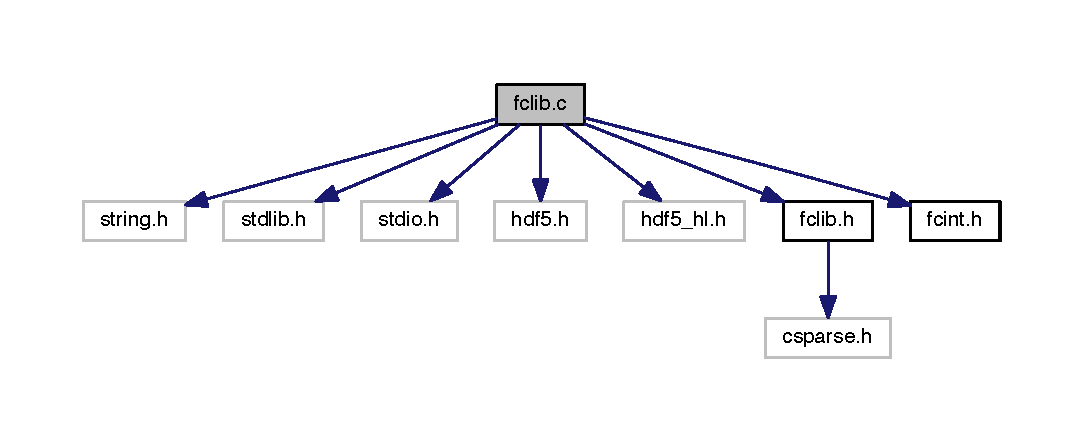
\includegraphics[width=350pt]{fclib_8c__incl}
\end{center}
\end{figure}
\subsubsection*{Macros}
\begin{DoxyCompactItemize}
\item 
\#define \hyperlink{fclib_8c_ae8ec3114e7970ceac40260041d66edbb}{H5\+Gcreate\+\_\+vers}~2
\item 
\#define \hyperlink{fclib_8c_a76c98e4e3ad7bd3a5a480e59f446d20d}{H5\+Gopen\+\_\+vers}~2
\end{DoxyCompactItemize}
\subsubsection*{Functions}
\begin{DoxyCompactItemize}
\item 
static hid\+\_\+t \hyperlink{fclib_8c_a59a656449b319a4517bb7e3c95efcb5d}{H5\+Gmake} (hid\+\_\+t loc\+\_\+id, const char $\ast$name)
\begin{DoxyCompactList}\small\item\em make grourp \end{DoxyCompactList}\item 
static void \hyperlink{fclib_8c_aefffb8708bf8509b7832d3ed70d4be47}{write\+\_\+matrix} (hid\+\_\+t id, struct \hyperlink{structfclib__matrix}{fclib\+\_\+matrix} $\ast$mat)
\begin{DoxyCompactList}\small\item\em write matrix \end{DoxyCompactList}\item 
struct \hyperlink{structfclib__matrix}{fclib\+\_\+matrix} $\ast$ \hyperlink{fclib_8c_a39c7990d9fd2ab18430feb9814c1e69d}{read\+\_\+matrix} (hid\+\_\+t id)
\begin{DoxyCompactList}\small\item\em read matrix \end{DoxyCompactList}\item 
static void \hyperlink{fclib_8c_a7834ca369ef4dd197d0667954854edd0}{write\+\_\+global\+\_\+vectors} (hid\+\_\+t id, struct \hyperlink{structfclib__global}{fclib\+\_\+global} $\ast$problem)
\begin{DoxyCompactList}\small\item\em write global vectors \end{DoxyCompactList}\item 
static void \hyperlink{fclib_8c_a7c692e0eee1727bb5a3033bd2330d81c}{read\+\_\+global\+\_\+vectors} (hid\+\_\+t id, struct \hyperlink{structfclib__global}{fclib\+\_\+global} $\ast$problem)
\begin{DoxyCompactList}\small\item\em read global vectors \end{DoxyCompactList}\item 
static void \hyperlink{fclib_8c_a6dcbbbee29d6a0af12fb87d531508a48}{write\+\_\+local\+\_\+vectors} (hid\+\_\+t id, struct \hyperlink{structfclib__local}{fclib\+\_\+local} $\ast$problem)
\begin{DoxyCompactList}\small\item\em write local vectors \end{DoxyCompactList}\item 
static void \hyperlink{fclib_8c_a8bc238e193fcdf7574221d62af6591c2}{read\+\_\+local\+\_\+vectors} (hid\+\_\+t id, struct \hyperlink{structfclib__local}{fclib\+\_\+local} $\ast$problem)
\begin{DoxyCompactList}\small\item\em read local vectors \end{DoxyCompactList}\item 
static void \hyperlink{fclib_8c_aca8c24ddc0ea386c97b678b1324ea0d4}{write\+\_\+problem\+\_\+info} (hid\+\_\+t id, struct \hyperlink{structfclib__info}{fclib\+\_\+info} $\ast$info)
\begin{DoxyCompactList}\small\item\em write problem info \end{DoxyCompactList}\item 
static struct \hyperlink{structfclib__info}{fclib\+\_\+info} $\ast$ \hyperlink{fclib_8c_a027ca7a38adea4ea55cd4ad3af71505d}{read\+\_\+problem\+\_\+info} (hid\+\_\+t id)
\begin{DoxyCompactList}\small\item\em read problem info \end{DoxyCompactList}\item 
static void \hyperlink{fclib_8c_aa4bc76f00cee23457c4f29ec53f8ceea}{write\+\_\+solution} (hid\+\_\+t id, struct \hyperlink{structfclib__solution}{fclib\+\_\+solution} $\ast$solution, hsize\+\_\+t nv, hsize\+\_\+t nr, hsize\+\_\+t nl)
\begin{DoxyCompactList}\small\item\em write solution \end{DoxyCompactList}\item 
static void \hyperlink{fclib_8c_af66ff03f18b03083ea7ad5a9ee9d2021}{read\+\_\+solution} (hid\+\_\+t id, hsize\+\_\+t nv, hsize\+\_\+t nr, hsize\+\_\+t nl, struct \hyperlink{structfclib__solution}{fclib\+\_\+solution} $\ast$solution)
\begin{DoxyCompactList}\small\item\em read solution \end{DoxyCompactList}\item 
static int \hyperlink{fclib_8c_a0da0a5e09f832f89656ad0fe8fc7064d}{read\+\_\+nvnunrnl} (hid\+\_\+t file\+\_\+id, int $\ast$nv, int $\ast$nr, int $\ast$nl)
\begin{DoxyCompactList}\small\item\em read solution sizes \end{DoxyCompactList}\item 
static void \hyperlink{fclib_8c_ac35480502e8612c3717d5fc6279de0c5}{delete\+\_\+matrix\+\_\+info} (struct \hyperlink{structfclib__matrix__info}{fclib\+\_\+matrix\+\_\+info} $\ast$info)
\begin{DoxyCompactList}\small\item\em delete matrix info \end{DoxyCompactList}\item 
static void \hyperlink{fclib_8c_ab5f8fb6fdbd5d68d93e1b68e8b009581}{delete\+\_\+matrix} (struct \hyperlink{structfclib__matrix}{fclib\+\_\+matrix} $\ast$mat)
\begin{DoxyCompactList}\small\item\em delete matrix \end{DoxyCompactList}\item 
static void \hyperlink{fclib_8c_a0b6e96725a6f98fdd3b49cdaea3aa38d}{delete\+\_\+info} (struct \hyperlink{structfclib__info}{fclib\+\_\+info} $\ast$info)
\begin{DoxyCompactList}\small\item\em delete problem info \end{DoxyCompactList}\item 
int \hyperlink{fclib_8c_a8b3c88579db667d89aa7d7a6c6fd90f4}{fclib\+\_\+create\+\_\+int\+\_\+attributes\+\_\+in\+\_\+info} (const char $\ast$path, const char $\ast$attr\+\_\+name, int attr\+\_\+value)
\begin{DoxyCompactList}\small\item\em create and set attributes of tyoe int in info \end{DoxyCompactList}\item 
int \hyperlink{fclib_8c_acd5a38f03c621ce4a53eea28ae6d9e2e}{fclib\+\_\+write\+\_\+global} (struct \hyperlink{structfclib__global}{fclib\+\_\+global} $\ast$problem, const char $\ast$path)
\begin{DoxyCompactList}\small\item\em write global problem; return 1 on success, 0 on failure \end{DoxyCompactList}\item 
int \hyperlink{fclib_8c_a5c4c7bb4d98efc388fdf4a7aa009b87a}{fclib\+\_\+write\+\_\+local} (struct \hyperlink{structfclib__local}{fclib\+\_\+local} $\ast$problem, const char $\ast$path)
\begin{DoxyCompactList}\small\item\em write local problem; return 1 on success, 0 on failure \end{DoxyCompactList}\item 
int \hyperlink{fclib_8c_a6edc26abbeec9f3e9a4fa71e70726988}{fclib\+\_\+write\+\_\+solution} (struct \hyperlink{structfclib__solution}{fclib\+\_\+solution} $\ast$solution, const char $\ast$path)
\begin{DoxyCompactList}\small\item\em write solution; return 1 on success, 0 on failure \end{DoxyCompactList}\item 
int \hyperlink{fclib_8c_a5100104b958b245b883f5d505651a5c1}{fclib\+\_\+write\+\_\+guesses} (int number\+\_\+of\+\_\+guesses, struct \hyperlink{structfclib__solution}{fclib\+\_\+solution} $\ast$guesses, const char $\ast$path)
\begin{DoxyCompactList}\small\item\em write initial guesses; return 1 on success, 0 on failure \end{DoxyCompactList}\item 
struct \hyperlink{structfclib__global}{fclib\+\_\+global} $\ast$ \hyperlink{fclib_8c_a68650a3ef8e5cfca61e10ede3ff59745}{fclib\+\_\+read\+\_\+global} (const char $\ast$path)
\begin{DoxyCompactList}\small\item\em read global problem; return problem on success; N\+U\+L\+L on failure \end{DoxyCompactList}\item 
struct \hyperlink{structfclib__local}{fclib\+\_\+local} $\ast$ \hyperlink{fclib_8c_a1122778ddd33ab84360ec6da584bff99}{fclib\+\_\+read\+\_\+local} (const char $\ast$path)
\begin{DoxyCompactList}\small\item\em read local problem; return problem on success; N\+U\+L\+L on failure \end{DoxyCompactList}\item 
struct \hyperlink{structfclib__solution}{fclib\+\_\+solution} $\ast$ \hyperlink{fclib_8c_a038c74114b0d53fd79785d99cd6c42fb}{fclib\+\_\+read\+\_\+solution} (const char $\ast$path)
\begin{DoxyCompactList}\small\item\em read solution; return solution on success; N\+U\+L\+L on failure \end{DoxyCompactList}\item 
struct \hyperlink{structfclib__solution}{fclib\+\_\+solution} $\ast$ \hyperlink{fclib_8c_ad1392d4746f60eb0030d6f9e80846e53}{fclib\+\_\+read\+\_\+guesses} (const char $\ast$path, int $\ast$number\+\_\+of\+\_\+guesses)
\begin{DoxyCompactList}\small\item\em read initial guesses; return vector of guesses on success; N\+U\+L\+L on failure; output numebr of guesses in the variable pointed by \textquotesingle{}number\+\_\+of\+\_\+guesses\textquotesingle{} \end{DoxyCompactList}\item 
void \hyperlink{fclib_8c_a14b1c35f51633d79f4ed6a680d21d6b4}{fclib\+\_\+delete\+\_\+global} (struct \hyperlink{structfclib__global}{fclib\+\_\+global} $\ast$problem)
\begin{DoxyCompactList}\small\item\em delete global problem \end{DoxyCompactList}\item 
void \hyperlink{fclib_8c_a20292c502d574d412fd8b41aad37225b}{fclib\+\_\+delete\+\_\+local} (struct \hyperlink{structfclib__local}{fclib\+\_\+local} $\ast$problem)
\begin{DoxyCompactList}\small\item\em delete local problem \end{DoxyCompactList}\item 
void \hyperlink{fclib_8c_a4b70826ccf4a67808e1946036ac6d950}{fclib\+\_\+delete\+\_\+solutions} (struct \hyperlink{structfclib__solution}{fclib\+\_\+solution} $\ast$data, int count)
\begin{DoxyCompactList}\small\item\em delete solutions or guesses \end{DoxyCompactList}\end{DoxyCompactItemize}


\subsubsection{Detailed Description}


 frictional contact library input/output 

\subsubsection{Macro Definition Documentation}
\hypertarget{fclib_8c_ae8ec3114e7970ceac40260041d66edbb}{}\index{fclib.\+c@{fclib.\+c}!H5\+Gcreate\+\_\+vers@{H5\+Gcreate\+\_\+vers}}
\index{H5\+Gcreate\+\_\+vers@{H5\+Gcreate\+\_\+vers}!fclib.\+c@{fclib.\+c}}
\paragraph[{H5\+Gcreate\+\_\+vers}]{\setlength{\rightskip}{0pt plus 5cm}\#define H5\+Gcreate\+\_\+vers~2}\label{fclib_8c_ae8ec3114e7970ceac40260041d66edbb}


Definition at line 24 of file fclib.\+c.

\hypertarget{fclib_8c_a76c98e4e3ad7bd3a5a480e59f446d20d}{}\index{fclib.\+c@{fclib.\+c}!H5\+Gopen\+\_\+vers@{H5\+Gopen\+\_\+vers}}
\index{H5\+Gopen\+\_\+vers@{H5\+Gopen\+\_\+vers}!fclib.\+c@{fclib.\+c}}
\paragraph[{H5\+Gopen\+\_\+vers}]{\setlength{\rightskip}{0pt plus 5cm}\#define H5\+Gopen\+\_\+vers~2}\label{fclib_8c_a76c98e4e3ad7bd3a5a480e59f446d20d}


Definition at line 25 of file fclib.\+c.



\subsubsection{Function Documentation}
\hypertarget{fclib_8c_a59a656449b319a4517bb7e3c95efcb5d}{}\index{fclib.\+c@{fclib.\+c}!H5\+Gmake@{H5\+Gmake}}
\index{H5\+Gmake@{H5\+Gmake}!fclib.\+c@{fclib.\+c}}
\paragraph[{H5\+Gmake(hid\+\_\+t loc\+\_\+id, const char $\ast$name)}]{\setlength{\rightskip}{0pt plus 5cm}static hid\+\_\+t H5\+Gmake (
\begin{DoxyParamCaption}
\item[{hid\+\_\+t}]{loc\+\_\+id, }
\item[{const char $\ast$}]{name}
\end{DoxyParamCaption}
)\hspace{0.3cm}{\ttfamily [static]}}\label{fclib_8c_a59a656449b319a4517bb7e3c95efcb5d}


make grourp 



Definition at line 37 of file fclib.\+c.



Referenced by fclib\+\_\+create\+\_\+int\+\_\+attributes\+\_\+in\+\_\+info(), fclib\+\_\+write\+\_\+global(), fclib\+\_\+write\+\_\+guesses(), fclib\+\_\+write\+\_\+local(), and fclib\+\_\+write\+\_\+solution().

\hypertarget{fclib_8c_aefffb8708bf8509b7832d3ed70d4be47}{}\index{fclib.\+c@{fclib.\+c}!write\+\_\+matrix@{write\+\_\+matrix}}
\index{write\+\_\+matrix@{write\+\_\+matrix}!fclib.\+c@{fclib.\+c}}
\paragraph[{write\+\_\+matrix(hid\+\_\+t id, struct fclib\+\_\+matrix $\ast$mat)}]{\setlength{\rightskip}{0pt plus 5cm}static void write\+\_\+matrix (
\begin{DoxyParamCaption}
\item[{hid\+\_\+t}]{id, }
\item[{struct {\bf fclib\+\_\+matrix} $\ast$}]{mat}
\end{DoxyParamCaption}
)\hspace{0.3cm}{\ttfamily [static]}}\label{fclib_8c_aefffb8708bf8509b7832d3ed70d4be47}


write matrix 



Definition at line 51 of file fclib.\+c.



References A\+S\+S\+E\+R\+T, fclib\+\_\+matrix\+\_\+info\+::comment, fclib\+\_\+matrix\+\_\+info\+::conditioning, fclib\+\_\+matrix\+\_\+info\+::determinant, fclib\+\_\+matrix\+::i, fclib\+\_\+matrix\+::info, I\+O, fclib\+\_\+matrix\+::m, fclib\+\_\+matrix\+::n, fclib\+\_\+matrix\+::nz, fclib\+\_\+matrix\+::nzmax, fclib\+\_\+matrix\+::p, fclib\+\_\+matrix\+\_\+info\+::rank, and fclib\+\_\+matrix\+::x.



Referenced by fclib\+\_\+write\+\_\+global(), and fclib\+\_\+write\+\_\+local().

\hypertarget{fclib_8c_a39c7990d9fd2ab18430feb9814c1e69d}{}\index{fclib.\+c@{fclib.\+c}!read\+\_\+matrix@{read\+\_\+matrix}}
\index{read\+\_\+matrix@{read\+\_\+matrix}!fclib.\+c@{fclib.\+c}}
\paragraph[{read\+\_\+matrix(hid\+\_\+t id)}]{\setlength{\rightskip}{0pt plus 5cm}struct {\bf fclib\+\_\+matrix}$\ast$ read\+\_\+matrix (
\begin{DoxyParamCaption}
\item[{hid\+\_\+t}]{id}
\end{DoxyParamCaption}
)}\label{fclib_8c_a39c7990d9fd2ab18430feb9814c1e69d}


read matrix 



Definition at line 96 of file fclib.\+c.



References A\+S\+S\+E\+R\+T, fclib\+\_\+matrix\+\_\+info\+::comment, fclib\+\_\+matrix\+\_\+info\+::conditioning, fclib\+\_\+matrix\+\_\+info\+::determinant, fclib\+\_\+matrix\+::i, fclib\+\_\+matrix\+::info, I\+O, fclib\+\_\+matrix\+::m, M\+M, fclib\+\_\+matrix\+::n, fclib\+\_\+matrix\+::nz, fclib\+\_\+matrix\+::nzmax, fclib\+\_\+matrix\+::p, fclib\+\_\+matrix\+\_\+info\+::rank, and fclib\+\_\+matrix\+::x.



Referenced by fclib\+\_\+read\+\_\+global(), and fclib\+\_\+read\+\_\+local().

\hypertarget{fclib_8c_a7834ca369ef4dd197d0667954854edd0}{}\index{fclib.\+c@{fclib.\+c}!write\+\_\+global\+\_\+vectors@{write\+\_\+global\+\_\+vectors}}
\index{write\+\_\+global\+\_\+vectors@{write\+\_\+global\+\_\+vectors}!fclib.\+c@{fclib.\+c}}
\paragraph[{write\+\_\+global\+\_\+vectors(hid\+\_\+t id, struct fclib\+\_\+global $\ast$problem)}]{\setlength{\rightskip}{0pt plus 5cm}static void write\+\_\+global\+\_\+vectors (
\begin{DoxyParamCaption}
\item[{hid\+\_\+t}]{id, }
\item[{struct {\bf fclib\+\_\+global} $\ast$}]{problem}
\end{DoxyParamCaption}
)\hspace{0.3cm}{\ttfamily [static]}}\label{fclib_8c_a7834ca369ef4dd197d0667954854edd0}


write global vectors 



Definition at line 156 of file fclib.\+c.



References A\+S\+S\+E\+R\+T, fclib\+\_\+global\+::b, fclib\+\_\+global\+::f, fclib\+\_\+global\+::\+G, fclib\+\_\+global\+::\+H, I\+O, fclib\+\_\+matrix\+::m, fclib\+\_\+global\+::\+M, fclib\+\_\+global\+::mu, fclib\+\_\+matrix\+::n, fclib\+\_\+global\+::spacedim, and fclib\+\_\+global\+::w.



Referenced by fclib\+\_\+write\+\_\+global().

\hypertarget{fclib_8c_a7c692e0eee1727bb5a3033bd2330d81c}{}\index{fclib.\+c@{fclib.\+c}!read\+\_\+global\+\_\+vectors@{read\+\_\+global\+\_\+vectors}}
\index{read\+\_\+global\+\_\+vectors@{read\+\_\+global\+\_\+vectors}!fclib.\+c@{fclib.\+c}}
\paragraph[{read\+\_\+global\+\_\+vectors(hid\+\_\+t id, struct fclib\+\_\+global $\ast$problem)}]{\setlength{\rightskip}{0pt plus 5cm}static void read\+\_\+global\+\_\+vectors (
\begin{DoxyParamCaption}
\item[{hid\+\_\+t}]{id, }
\item[{struct {\bf fclib\+\_\+global} $\ast$}]{problem}
\end{DoxyParamCaption}
)\hspace{0.3cm}{\ttfamily [static]}}\label{fclib_8c_a7c692e0eee1727bb5a3033bd2330d81c}


read global vectors 



Definition at line 180 of file fclib.\+c.



References A\+S\+S\+E\+R\+T, fclib\+\_\+global\+::b, fclib\+\_\+global\+::f, fclib\+\_\+global\+::\+G, fclib\+\_\+global\+::\+H, I\+O, fclib\+\_\+matrix\+::m, fclib\+\_\+global\+::\+M, M\+M, fclib\+\_\+global\+::mu, fclib\+\_\+matrix\+::n, fclib\+\_\+global\+::spacedim, and fclib\+\_\+global\+::w.



Referenced by fclib\+\_\+read\+\_\+global().

\hypertarget{fclib_8c_a6dcbbbee29d6a0af12fb87d531508a48}{}\index{fclib.\+c@{fclib.\+c}!write\+\_\+local\+\_\+vectors@{write\+\_\+local\+\_\+vectors}}
\index{write\+\_\+local\+\_\+vectors@{write\+\_\+local\+\_\+vectors}!fclib.\+c@{fclib.\+c}}
\paragraph[{write\+\_\+local\+\_\+vectors(hid\+\_\+t id, struct fclib\+\_\+local $\ast$problem)}]{\setlength{\rightskip}{0pt plus 5cm}static void write\+\_\+local\+\_\+vectors (
\begin{DoxyParamCaption}
\item[{hid\+\_\+t}]{id, }
\item[{struct {\bf fclib\+\_\+local} $\ast$}]{problem}
\end{DoxyParamCaption}
)\hspace{0.3cm}{\ttfamily [static]}}\label{fclib_8c_a6dcbbbee29d6a0af12fb87d531508a48}


write local vectors 



Definition at line 199 of file fclib.\+c.



References A\+S\+S\+E\+R\+T, I\+O, fclib\+\_\+matrix\+::m, fclib\+\_\+local\+::mu, fclib\+\_\+local\+::q, fclib\+\_\+local\+::\+R, fclib\+\_\+local\+::s, fclib\+\_\+local\+::spacedim, fclib\+\_\+local\+::\+V, and fclib\+\_\+local\+::\+W.



Referenced by fclib\+\_\+write\+\_\+local().

\hypertarget{fclib_8c_a8bc238e193fcdf7574221d62af6591c2}{}\index{fclib.\+c@{fclib.\+c}!read\+\_\+local\+\_\+vectors@{read\+\_\+local\+\_\+vectors}}
\index{read\+\_\+local\+\_\+vectors@{read\+\_\+local\+\_\+vectors}!fclib.\+c@{fclib.\+c}}
\paragraph[{read\+\_\+local\+\_\+vectors(hid\+\_\+t id, struct fclib\+\_\+local $\ast$problem)}]{\setlength{\rightskip}{0pt plus 5cm}static void read\+\_\+local\+\_\+vectors (
\begin{DoxyParamCaption}
\item[{hid\+\_\+t}]{id, }
\item[{struct {\bf fclib\+\_\+local} $\ast$}]{problem}
\end{DoxyParamCaption}
)\hspace{0.3cm}{\ttfamily [static]}}\label{fclib_8c_a8bc238e193fcdf7574221d62af6591c2}


read local vectors 



Definition at line 220 of file fclib.\+c.



References A\+S\+S\+E\+R\+T, I\+O, fclib\+\_\+matrix\+::m, M\+M, fclib\+\_\+local\+::mu, fclib\+\_\+local\+::q, fclib\+\_\+local\+::\+R, fclib\+\_\+local\+::s, fclib\+\_\+local\+::spacedim, and fclib\+\_\+local\+::\+W.



Referenced by fclib\+\_\+read\+\_\+local().

\hypertarget{fclib_8c_aca8c24ddc0ea386c97b678b1324ea0d4}{}\index{fclib.\+c@{fclib.\+c}!write\+\_\+problem\+\_\+info@{write\+\_\+problem\+\_\+info}}
\index{write\+\_\+problem\+\_\+info@{write\+\_\+problem\+\_\+info}!fclib.\+c@{fclib.\+c}}
\paragraph[{write\+\_\+problem\+\_\+info(hid\+\_\+t id, struct fclib\+\_\+info $\ast$info)}]{\setlength{\rightskip}{0pt plus 5cm}static void write\+\_\+problem\+\_\+info (
\begin{DoxyParamCaption}
\item[{hid\+\_\+t}]{id, }
\item[{struct {\bf fclib\+\_\+info} $\ast$}]{info}
\end{DoxyParamCaption}
)\hspace{0.3cm}{\ttfamily [static]}}\label{fclib_8c_aca8c24ddc0ea386c97b678b1324ea0d4}


write problem info 



Definition at line 237 of file fclib.\+c.



References fclib\+\_\+info\+::description, I\+O, fclib\+\_\+info\+::math\+\_\+info, and fclib\+\_\+info\+::title.



Referenced by fclib\+\_\+write\+\_\+global(), and fclib\+\_\+write\+\_\+local().

\hypertarget{fclib_8c_a027ca7a38adea4ea55cd4ad3af71505d}{}\index{fclib.\+c@{fclib.\+c}!read\+\_\+problem\+\_\+info@{read\+\_\+problem\+\_\+info}}
\index{read\+\_\+problem\+\_\+info@{read\+\_\+problem\+\_\+info}!fclib.\+c@{fclib.\+c}}
\paragraph[{read\+\_\+problem\+\_\+info(hid\+\_\+t id)}]{\setlength{\rightskip}{0pt plus 5cm}static struct {\bf fclib\+\_\+info}$\ast$ read\+\_\+problem\+\_\+info (
\begin{DoxyParamCaption}
\item[{hid\+\_\+t}]{id}
\end{DoxyParamCaption}
)\hspace{0.3cm}{\ttfamily [static]}}\label{fclib_8c_a027ca7a38adea4ea55cd4ad3af71505d}


read problem info 



Definition at line 245 of file fclib.\+c.



References fclib\+\_\+info\+::description, I\+O, fclib\+\_\+info\+::math\+\_\+info, M\+M, and fclib\+\_\+info\+::title.



Referenced by fclib\+\_\+read\+\_\+global(), and fclib\+\_\+read\+\_\+local().

\hypertarget{fclib_8c_aa4bc76f00cee23457c4f29ec53f8ceea}{}\index{fclib.\+c@{fclib.\+c}!write\+\_\+solution@{write\+\_\+solution}}
\index{write\+\_\+solution@{write\+\_\+solution}!fclib.\+c@{fclib.\+c}}
\paragraph[{write\+\_\+solution(hid\+\_\+t id, struct fclib\+\_\+solution $\ast$solution, hsize\+\_\+t nv, hsize\+\_\+t nr, hsize\+\_\+t nl)}]{\setlength{\rightskip}{0pt plus 5cm}static void write\+\_\+solution (
\begin{DoxyParamCaption}
\item[{hid\+\_\+t}]{id, }
\item[{struct {\bf fclib\+\_\+solution} $\ast$}]{solution, }
\item[{hsize\+\_\+t}]{nv, }
\item[{hsize\+\_\+t}]{nr, }
\item[{hsize\+\_\+t}]{nl}
\end{DoxyParamCaption}
)\hspace{0.3cm}{\ttfamily [static]}}\label{fclib_8c_aa4bc76f00cee23457c4f29ec53f8ceea}


write solution 



Definition at line 282 of file fclib.\+c.



References A\+S\+S\+E\+R\+T, I\+O, fclib\+\_\+solution\+::l, fclib\+\_\+solution\+::r, fclib\+\_\+solution\+::u, and fclib\+\_\+solution\+::v.



Referenced by fclib\+\_\+write\+\_\+guesses(), and fclib\+\_\+write\+\_\+solution().

\hypertarget{fclib_8c_af66ff03f18b03083ea7ad5a9ee9d2021}{}\index{fclib.\+c@{fclib.\+c}!read\+\_\+solution@{read\+\_\+solution}}
\index{read\+\_\+solution@{read\+\_\+solution}!fclib.\+c@{fclib.\+c}}
\paragraph[{read\+\_\+solution(hid\+\_\+t id, hsize\+\_\+t nv, hsize\+\_\+t nr, hsize\+\_\+t nl, struct fclib\+\_\+solution $\ast$solution)}]{\setlength{\rightskip}{0pt plus 5cm}static void read\+\_\+solution (
\begin{DoxyParamCaption}
\item[{hid\+\_\+t}]{id, }
\item[{hsize\+\_\+t}]{nv, }
\item[{hsize\+\_\+t}]{nr, }
\item[{hsize\+\_\+t}]{nl, }
\item[{struct {\bf fclib\+\_\+solution} $\ast$}]{solution}
\end{DoxyParamCaption}
)\hspace{0.3cm}{\ttfamily [static]}}\label{fclib_8c_af66ff03f18b03083ea7ad5a9ee9d2021}


read solution 



Definition at line 293 of file fclib.\+c.



References A\+S\+S\+E\+R\+T, I\+O, fclib\+\_\+solution\+::l, M\+M, fclib\+\_\+solution\+::r, fclib\+\_\+solution\+::u, and fclib\+\_\+solution\+::v.



Referenced by fclib\+\_\+read\+\_\+guesses(), and fclib\+\_\+read\+\_\+solution().

\hypertarget{fclib_8c_a0da0a5e09f832f89656ad0fe8fc7064d}{}\index{fclib.\+c@{fclib.\+c}!read\+\_\+nvnunrnl@{read\+\_\+nvnunrnl}}
\index{read\+\_\+nvnunrnl@{read\+\_\+nvnunrnl}!fclib.\+c@{fclib.\+c}}
\paragraph[{read\+\_\+nvnunrnl(hid\+\_\+t file\+\_\+id, int $\ast$nv, int $\ast$nr, int $\ast$nl)}]{\setlength{\rightskip}{0pt plus 5cm}static int read\+\_\+nvnunrnl (
\begin{DoxyParamCaption}
\item[{hid\+\_\+t}]{file\+\_\+id, }
\item[{int $\ast$}]{nv, }
\item[{int $\ast$}]{nr, }
\item[{int $\ast$}]{nl}
\end{DoxyParamCaption}
)\hspace{0.3cm}{\ttfamily [static]}}\label{fclib_8c_a0da0a5e09f832f89656ad0fe8fc7064d}


read solution sizes 



Definition at line 317 of file fclib.\+c.



References I\+O.



Referenced by fclib\+\_\+read\+\_\+guesses(), fclib\+\_\+read\+\_\+solution(), fclib\+\_\+write\+\_\+guesses(), and fclib\+\_\+write\+\_\+solution().

\hypertarget{fclib_8c_ac35480502e8612c3717d5fc6279de0c5}{}\index{fclib.\+c@{fclib.\+c}!delete\+\_\+matrix\+\_\+info@{delete\+\_\+matrix\+\_\+info}}
\index{delete\+\_\+matrix\+\_\+info@{delete\+\_\+matrix\+\_\+info}!fclib.\+c@{fclib.\+c}}
\paragraph[{delete\+\_\+matrix\+\_\+info(struct fclib\+\_\+matrix\+\_\+info $\ast$info)}]{\setlength{\rightskip}{0pt plus 5cm}static void delete\+\_\+matrix\+\_\+info (
\begin{DoxyParamCaption}
\item[{struct {\bf fclib\+\_\+matrix\+\_\+info} $\ast$}]{info}
\end{DoxyParamCaption}
)\hspace{0.3cm}{\ttfamily [static]}}\label{fclib_8c_ac35480502e8612c3717d5fc6279de0c5}


delete matrix info 



Definition at line 349 of file fclib.\+c.



References fclib\+\_\+matrix\+\_\+info\+::comment.



Referenced by delete\+\_\+matrix().

\hypertarget{fclib_8c_ab5f8fb6fdbd5d68d93e1b68e8b009581}{}\index{fclib.\+c@{fclib.\+c}!delete\+\_\+matrix@{delete\+\_\+matrix}}
\index{delete\+\_\+matrix@{delete\+\_\+matrix}!fclib.\+c@{fclib.\+c}}
\paragraph[{delete\+\_\+matrix(struct fclib\+\_\+matrix $\ast$mat)}]{\setlength{\rightskip}{0pt plus 5cm}static void delete\+\_\+matrix (
\begin{DoxyParamCaption}
\item[{struct {\bf fclib\+\_\+matrix} $\ast$}]{mat}
\end{DoxyParamCaption}
)\hspace{0.3cm}{\ttfamily [static]}}\label{fclib_8c_ab5f8fb6fdbd5d68d93e1b68e8b009581}


delete matrix 



Definition at line 359 of file fclib.\+c.



References delete\+\_\+matrix\+\_\+info(), fclib\+\_\+matrix\+::i, fclib\+\_\+matrix\+::info, fclib\+\_\+matrix\+::p, and fclib\+\_\+matrix\+::x.



Referenced by fclib\+\_\+delete\+\_\+global(), and fclib\+\_\+delete\+\_\+local().



Here is the call graph for this function\+:\nopagebreak
\begin{figure}[H]
\begin{center}
\leavevmode
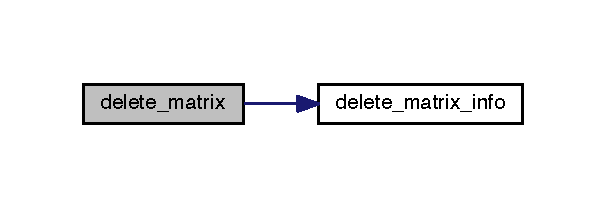
\includegraphics[width=291pt]{fclib_8c_ab5f8fb6fdbd5d68d93e1b68e8b009581_cgraph}
\end{center}
\end{figure}


\hypertarget{fclib_8c_a0b6e96725a6f98fdd3b49cdaea3aa38d}{}\index{fclib.\+c@{fclib.\+c}!delete\+\_\+info@{delete\+\_\+info}}
\index{delete\+\_\+info@{delete\+\_\+info}!fclib.\+c@{fclib.\+c}}
\paragraph[{delete\+\_\+info(struct fclib\+\_\+info $\ast$info)}]{\setlength{\rightskip}{0pt plus 5cm}static void delete\+\_\+info (
\begin{DoxyParamCaption}
\item[{struct {\bf fclib\+\_\+info} $\ast$}]{info}
\end{DoxyParamCaption}
)\hspace{0.3cm}{\ttfamily [static]}}\label{fclib_8c_a0b6e96725a6f98fdd3b49cdaea3aa38d}


delete problem info 



Definition at line 372 of file fclib.\+c.



References fclib\+\_\+info\+::description, fclib\+\_\+info\+::math\+\_\+info, and fclib\+\_\+info\+::title.



Referenced by fclib\+\_\+delete\+\_\+global(), and fclib\+\_\+delete\+\_\+local().

\hypertarget{fclib_8c_a8b3c88579db667d89aa7d7a6c6fd90f4}{}\index{fclib.\+c@{fclib.\+c}!fclib\+\_\+create\+\_\+int\+\_\+attributes\+\_\+in\+\_\+info@{fclib\+\_\+create\+\_\+int\+\_\+attributes\+\_\+in\+\_\+info}}
\index{fclib\+\_\+create\+\_\+int\+\_\+attributes\+\_\+in\+\_\+info@{fclib\+\_\+create\+\_\+int\+\_\+attributes\+\_\+in\+\_\+info}!fclib.\+c@{fclib.\+c}}
\paragraph[{fclib\+\_\+create\+\_\+int\+\_\+attributes\+\_\+in\+\_\+info(const char $\ast$path, const char $\ast$attr\+\_\+name, int attr\+\_\+value)}]{\setlength{\rightskip}{0pt plus 5cm}int fclib\+\_\+create\+\_\+int\+\_\+attributes\+\_\+in\+\_\+info (
\begin{DoxyParamCaption}
\item[{const char $\ast$}]{path, }
\item[{const char $\ast$}]{attr\+\_\+name, }
\item[{int}]{attr\+\_\+value}
\end{DoxyParamCaption}
)}\label{fclib_8c_a8b3c88579db667d89aa7d7a6c6fd90f4}


create and set attributes of tyoe int in info 



Definition at line 382 of file fclib.\+c.



References H5\+Gmake(), and I\+O.



Here is the call graph for this function\+:\nopagebreak
\begin{figure}[H]
\begin{center}
\leavevmode
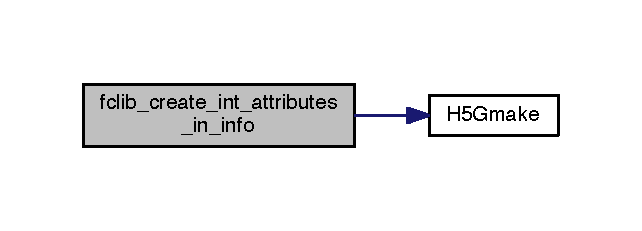
\includegraphics[width=308pt]{fclib_8c_a8b3c88579db667d89aa7d7a6c6fd90f4_cgraph}
\end{center}
\end{figure}


\hypertarget{fclib_8c_acd5a38f03c621ce4a53eea28ae6d9e2e}{}\index{fclib.\+c@{fclib.\+c}!fclib\+\_\+write\+\_\+global@{fclib\+\_\+write\+\_\+global}}
\index{fclib\+\_\+write\+\_\+global@{fclib\+\_\+write\+\_\+global}!fclib.\+c@{fclib.\+c}}
\paragraph[{fclib\+\_\+write\+\_\+global(struct fclib\+\_\+global $\ast$problem, const char $\ast$path)}]{\setlength{\rightskip}{0pt plus 5cm}int fclib\+\_\+write\+\_\+global (
\begin{DoxyParamCaption}
\item[{struct {\bf fclib\+\_\+global} $\ast$}]{problem, }
\item[{const char $\ast$}]{path}
\end{DoxyParamCaption}
)}\label{fclib_8c_acd5a38f03c621ce4a53eea28ae6d9e2e}


write global problem; return 1 on success, 0 on failure 



Definition at line 431 of file fclib.\+c.



References A\+S\+S\+E\+R\+T, fclib\+\_\+global\+::\+G, fclib\+\_\+global\+::\+H, H5\+Gmake(), fclib\+\_\+global\+::info, I\+O, fclib\+\_\+global\+::\+M, fclib\+\_\+global\+::spacedim, write\+\_\+global\+\_\+vectors(), write\+\_\+matrix(), and write\+\_\+problem\+\_\+info().



Referenced by main().



Here is the call graph for this function\+:\nopagebreak
\begin{figure}[H]
\begin{center}
\leavevmode
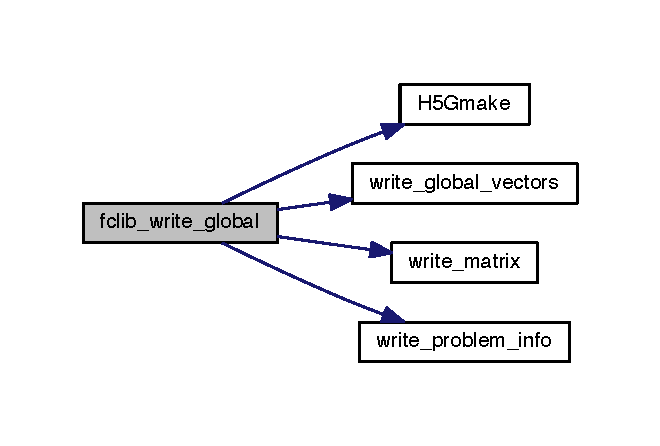
\includegraphics[width=317pt]{fclib_8c_acd5a38f03c621ce4a53eea28ae6d9e2e_cgraph}
\end{center}
\end{figure}


\hypertarget{fclib_8c_a5c4c7bb4d98efc388fdf4a7aa009b87a}{}\index{fclib.\+c@{fclib.\+c}!fclib\+\_\+write\+\_\+local@{fclib\+\_\+write\+\_\+local}}
\index{fclib\+\_\+write\+\_\+local@{fclib\+\_\+write\+\_\+local}!fclib.\+c@{fclib.\+c}}
\paragraph[{fclib\+\_\+write\+\_\+local(struct fclib\+\_\+local $\ast$problem, const char $\ast$path)}]{\setlength{\rightskip}{0pt plus 5cm}int fclib\+\_\+write\+\_\+local (
\begin{DoxyParamCaption}
\item[{struct {\bf fclib\+\_\+local} $\ast$}]{problem, }
\item[{const char $\ast$}]{path}
\end{DoxyParamCaption}
)}\label{fclib_8c_a5c4c7bb4d98efc388fdf4a7aa009b87a}


write local problem; return 1 on success, 0 on failure 



Definition at line 503 of file fclib.\+c.



References A\+S\+S\+E\+R\+T, H5\+Gmake(), fclib\+\_\+local\+::info, I\+O, fclib\+\_\+local\+::\+R, fclib\+\_\+local\+::spacedim, fclib\+\_\+local\+::\+V, fclib\+\_\+local\+::\+W, write\+\_\+local\+\_\+vectors(), write\+\_\+matrix(), and write\+\_\+problem\+\_\+info().



Referenced by main().



Here is the call graph for this function\+:\nopagebreak
\begin{figure}[H]
\begin{center}
\leavevmode
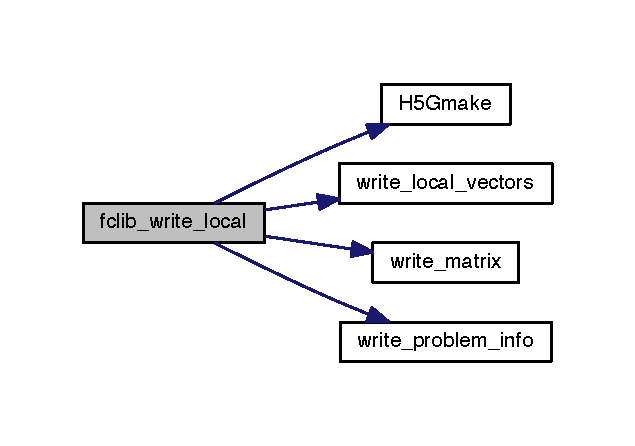
\includegraphics[width=305pt]{fclib_8c_a5c4c7bb4d98efc388fdf4a7aa009b87a_cgraph}
\end{center}
\end{figure}


\hypertarget{fclib_8c_a6edc26abbeec9f3e9a4fa71e70726988}{}\index{fclib.\+c@{fclib.\+c}!fclib\+\_\+write\+\_\+solution@{fclib\+\_\+write\+\_\+solution}}
\index{fclib\+\_\+write\+\_\+solution@{fclib\+\_\+write\+\_\+solution}!fclib.\+c@{fclib.\+c}}
\paragraph[{fclib\+\_\+write\+\_\+solution(struct fclib\+\_\+solution $\ast$solution, const char $\ast$path)}]{\setlength{\rightskip}{0pt plus 5cm}int fclib\+\_\+write\+\_\+solution (
\begin{DoxyParamCaption}
\item[{struct {\bf fclib\+\_\+solution} $\ast$}]{solution, }
\item[{const char $\ast$}]{path}
\end{DoxyParamCaption}
)}\label{fclib_8c_a6edc26abbeec9f3e9a4fa71e70726988}


write solution; return 1 on success, 0 on failure 



Definition at line 571 of file fclib.\+c.



References H5\+Gmake(), I\+O, read\+\_\+nvnunrnl(), and write\+\_\+solution().



Referenced by main().



Here is the call graph for this function\+:\nopagebreak
\begin{figure}[H]
\begin{center}
\leavevmode
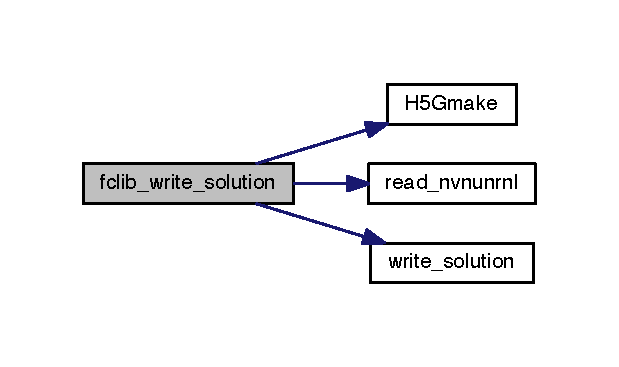
\includegraphics[width=297pt]{fclib_8c_a6edc26abbeec9f3e9a4fa71e70726988_cgraph}
\end{center}
\end{figure}


\hypertarget{fclib_8c_a5100104b958b245b883f5d505651a5c1}{}\index{fclib.\+c@{fclib.\+c}!fclib\+\_\+write\+\_\+guesses@{fclib\+\_\+write\+\_\+guesses}}
\index{fclib\+\_\+write\+\_\+guesses@{fclib\+\_\+write\+\_\+guesses}!fclib.\+c@{fclib.\+c}}
\paragraph[{fclib\+\_\+write\+\_\+guesses(int number\+\_\+of\+\_\+guesses, struct fclib\+\_\+solution $\ast$guesses, const char $\ast$path)}]{\setlength{\rightskip}{0pt plus 5cm}int fclib\+\_\+write\+\_\+guesses (
\begin{DoxyParamCaption}
\item[{int}]{number\+\_\+of\+\_\+guesses, }
\item[{struct {\bf fclib\+\_\+solution} $\ast$}]{guesses, }
\item[{const char $\ast$}]{path}
\end{DoxyParamCaption}
)}\label{fclib_8c_a5100104b958b245b883f5d505651a5c1}


write initial guesses; return 1 on success, 0 on failure 



Definition at line 611 of file fclib.\+c.



References H5\+Gmake(), I\+O, read\+\_\+nvnunrnl(), and write\+\_\+solution().



Referenced by main().



Here is the call graph for this function\+:\nopagebreak
\begin{figure}[H]
\begin{center}
\leavevmode
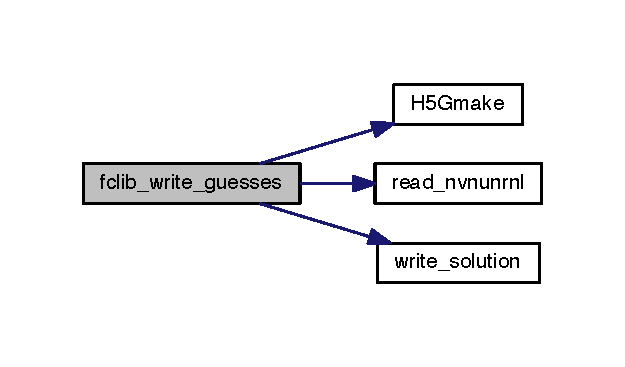
\includegraphics[width=300pt]{fclib_8c_a5100104b958b245b883f5d505651a5c1_cgraph}
\end{center}
\end{figure}


\hypertarget{fclib_8c_a68650a3ef8e5cfca61e10ede3ff59745}{}\index{fclib.\+c@{fclib.\+c}!fclib\+\_\+read\+\_\+global@{fclib\+\_\+read\+\_\+global}}
\index{fclib\+\_\+read\+\_\+global@{fclib\+\_\+read\+\_\+global}!fclib.\+c@{fclib.\+c}}
\paragraph[{fclib\+\_\+read\+\_\+global(const char $\ast$path)}]{\setlength{\rightskip}{0pt plus 5cm}struct {\bf fclib\+\_\+global}$\ast$ fclib\+\_\+read\+\_\+global (
\begin{DoxyParamCaption}
\item[{const char $\ast$}]{path}
\end{DoxyParamCaption}
)}\label{fclib_8c_a68650a3ef8e5cfca61e10ede3ff59745}


read global problem; return problem on success; N\+U\+L\+L on failure 



Definition at line 661 of file fclib.\+c.



References fclib\+\_\+global\+::\+G, fclib\+\_\+global\+::\+H, fclib\+\_\+global\+::info, I\+O, fclib\+\_\+global\+::\+M, M\+M, read\+\_\+global\+\_\+vectors(), read\+\_\+matrix(), read\+\_\+problem\+\_\+info(), and fclib\+\_\+global\+::spacedim.



Referenced by main().



Here is the call graph for this function\+:\nopagebreak
\begin{figure}[H]
\begin{center}
\leavevmode
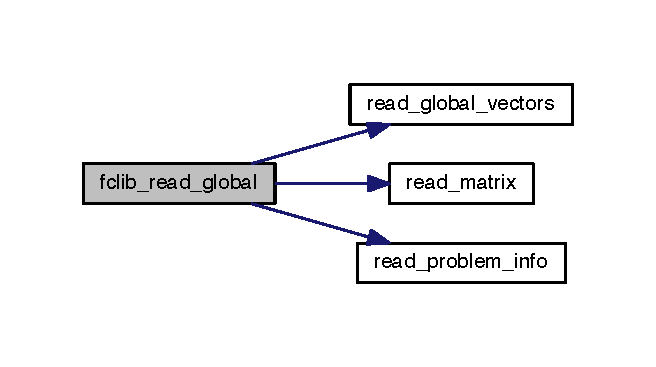
\includegraphics[width=315pt]{fclib_8c_a68650a3ef8e5cfca61e10ede3ff59745_cgraph}
\end{center}
\end{figure}


\hypertarget{fclib_8c_a1122778ddd33ab84360ec6da584bff99}{}\index{fclib.\+c@{fclib.\+c}!fclib\+\_\+read\+\_\+local@{fclib\+\_\+read\+\_\+local}}
\index{fclib\+\_\+read\+\_\+local@{fclib\+\_\+read\+\_\+local}!fclib.\+c@{fclib.\+c}}
\paragraph[{fclib\+\_\+read\+\_\+local(const char $\ast$path)}]{\setlength{\rightskip}{0pt plus 5cm}struct {\bf fclib\+\_\+local}$\ast$ fclib\+\_\+read\+\_\+local (
\begin{DoxyParamCaption}
\item[{const char $\ast$}]{path}
\end{DoxyParamCaption}
)}\label{fclib_8c_a1122778ddd33ab84360ec6da584bff99}


read local problem; return problem on success; N\+U\+L\+L on failure 



Definition at line 711 of file fclib.\+c.



References fclib\+\_\+local\+::info, I\+O, M\+M, fclib\+\_\+local\+::\+R, read\+\_\+local\+\_\+vectors(), read\+\_\+matrix(), read\+\_\+problem\+\_\+info(), fclib\+\_\+local\+::spacedim, fclib\+\_\+local\+::\+V, and fclib\+\_\+local\+::\+W.



Referenced by main().



Here is the call graph for this function\+:\nopagebreak
\begin{figure}[H]
\begin{center}
\leavevmode
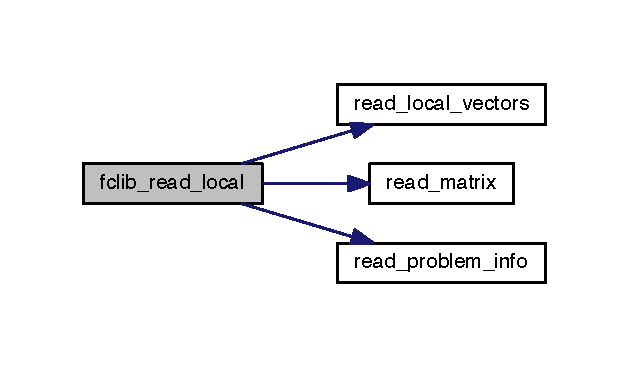
\includegraphics[width=302pt]{fclib_8c_a1122778ddd33ab84360ec6da584bff99_cgraph}
\end{center}
\end{figure}


\hypertarget{fclib_8c_a038c74114b0d53fd79785d99cd6c42fb}{}\index{fclib.\+c@{fclib.\+c}!fclib\+\_\+read\+\_\+solution@{fclib\+\_\+read\+\_\+solution}}
\index{fclib\+\_\+read\+\_\+solution@{fclib\+\_\+read\+\_\+solution}!fclib.\+c@{fclib.\+c}}
\paragraph[{fclib\+\_\+read\+\_\+solution(const char $\ast$path)}]{\setlength{\rightskip}{0pt plus 5cm}struct {\bf fclib\+\_\+solution}$\ast$ fclib\+\_\+read\+\_\+solution (
\begin{DoxyParamCaption}
\item[{const char $\ast$}]{path}
\end{DoxyParamCaption}
)}\label{fclib_8c_a038c74114b0d53fd79785d99cd6c42fb}


read solution; return solution on success; N\+U\+L\+L on failure 



Definition at line 761 of file fclib.\+c.



References I\+O, M\+M, read\+\_\+nvnunrnl(), and read\+\_\+solution().



Referenced by main().



Here is the call graph for this function\+:\nopagebreak
\begin{figure}[H]
\begin{center}
\leavevmode
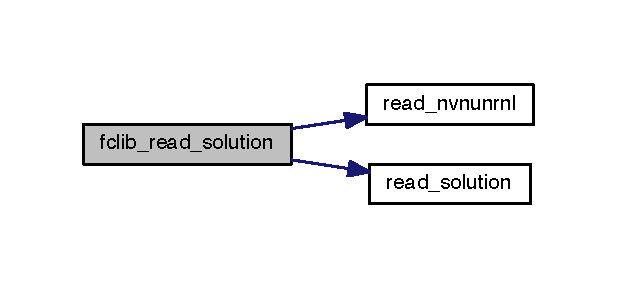
\includegraphics[width=296pt]{fclib_8c_a038c74114b0d53fd79785d99cd6c42fb_cgraph}
\end{center}
\end{figure}


\hypertarget{fclib_8c_ad1392d4746f60eb0030d6f9e80846e53}{}\index{fclib.\+c@{fclib.\+c}!fclib\+\_\+read\+\_\+guesses@{fclib\+\_\+read\+\_\+guesses}}
\index{fclib\+\_\+read\+\_\+guesses@{fclib\+\_\+read\+\_\+guesses}!fclib.\+c@{fclib.\+c}}
\paragraph[{fclib\+\_\+read\+\_\+guesses(const char $\ast$path, int $\ast$number\+\_\+of\+\_\+guesses)}]{\setlength{\rightskip}{0pt plus 5cm}struct {\bf fclib\+\_\+solution}$\ast$ fclib\+\_\+read\+\_\+guesses (
\begin{DoxyParamCaption}
\item[{const char $\ast$}]{path, }
\item[{int $\ast$}]{number\+\_\+of\+\_\+guesses}
\end{DoxyParamCaption}
)}\label{fclib_8c_ad1392d4746f60eb0030d6f9e80846e53}


read initial guesses; return vector of guesses on success; N\+U\+L\+L on failure; output numebr of guesses in the variable pointed by \textquotesingle{}number\+\_\+of\+\_\+guesses\textquotesingle{} 



Definition at line 789 of file fclib.\+c.



References I\+O, M\+M, read\+\_\+nvnunrnl(), and read\+\_\+solution().



Referenced by main().



Here is the call graph for this function\+:\nopagebreak
\begin{figure}[H]
\begin{center}
\leavevmode
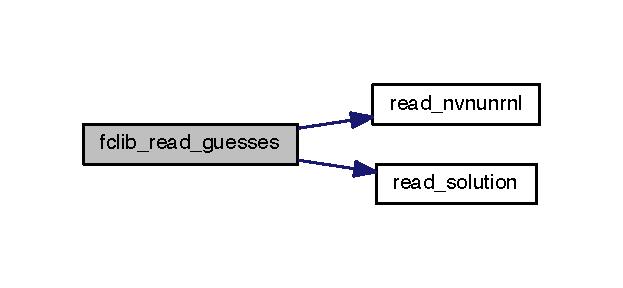
\includegraphics[width=299pt]{fclib_8c_ad1392d4746f60eb0030d6f9e80846e53_cgraph}
\end{center}
\end{figure}


\hypertarget{fclib_8c_a14b1c35f51633d79f4ed6a680d21d6b4}{}\index{fclib.\+c@{fclib.\+c}!fclib\+\_\+delete\+\_\+global@{fclib\+\_\+delete\+\_\+global}}
\index{fclib\+\_\+delete\+\_\+global@{fclib\+\_\+delete\+\_\+global}!fclib.\+c@{fclib.\+c}}
\paragraph[{fclib\+\_\+delete\+\_\+global(struct fclib\+\_\+global $\ast$problem)}]{\setlength{\rightskip}{0pt plus 5cm}void fclib\+\_\+delete\+\_\+global (
\begin{DoxyParamCaption}
\item[{struct {\bf fclib\+\_\+global} $\ast$}]{problem}
\end{DoxyParamCaption}
)}\label{fclib_8c_a14b1c35f51633d79f4ed6a680d21d6b4}


delete global problem 



Definition at line 829 of file fclib.\+c.



References fclib\+\_\+global\+::b, delete\+\_\+info(), delete\+\_\+matrix(), fclib\+\_\+global\+::f, fclib\+\_\+global\+::\+G, fclib\+\_\+global\+::\+H, fclib\+\_\+global\+::info, fclib\+\_\+global\+::\+M, fclib\+\_\+global\+::mu, and fclib\+\_\+global\+::w.



Referenced by main().



Here is the call graph for this function\+:\nopagebreak
\begin{figure}[H]
\begin{center}
\leavevmode
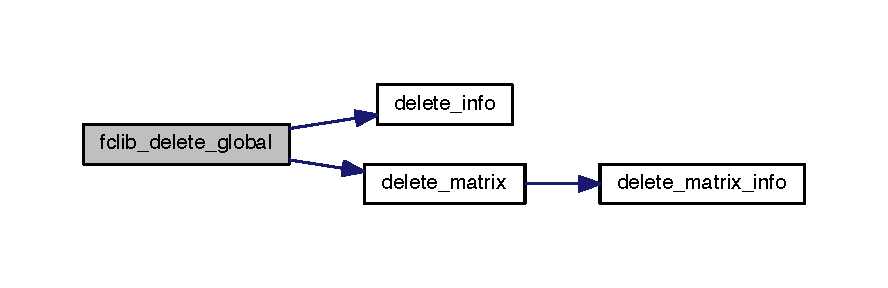
\includegraphics[width=350pt]{fclib_8c_a14b1c35f51633d79f4ed6a680d21d6b4_cgraph}
\end{center}
\end{figure}


\hypertarget{fclib_8c_a20292c502d574d412fd8b41aad37225b}{}\index{fclib.\+c@{fclib.\+c}!fclib\+\_\+delete\+\_\+local@{fclib\+\_\+delete\+\_\+local}}
\index{fclib\+\_\+delete\+\_\+local@{fclib\+\_\+delete\+\_\+local}!fclib.\+c@{fclib.\+c}}
\paragraph[{fclib\+\_\+delete\+\_\+local(struct fclib\+\_\+local $\ast$problem)}]{\setlength{\rightskip}{0pt plus 5cm}void fclib\+\_\+delete\+\_\+local (
\begin{DoxyParamCaption}
\item[{struct {\bf fclib\+\_\+local} $\ast$}]{problem}
\end{DoxyParamCaption}
)}\label{fclib_8c_a20292c502d574d412fd8b41aad37225b}


delete local problem 



Definition at line 842 of file fclib.\+c.



References delete\+\_\+info(), delete\+\_\+matrix(), fclib\+\_\+local\+::info, fclib\+\_\+local\+::mu, fclib\+\_\+local\+::q, fclib\+\_\+local\+::\+R, fclib\+\_\+local\+::s, fclib\+\_\+local\+::\+V, and fclib\+\_\+local\+::\+W.



Referenced by main().



Here is the call graph for this function\+:\nopagebreak
\begin{figure}[H]
\begin{center}
\leavevmode
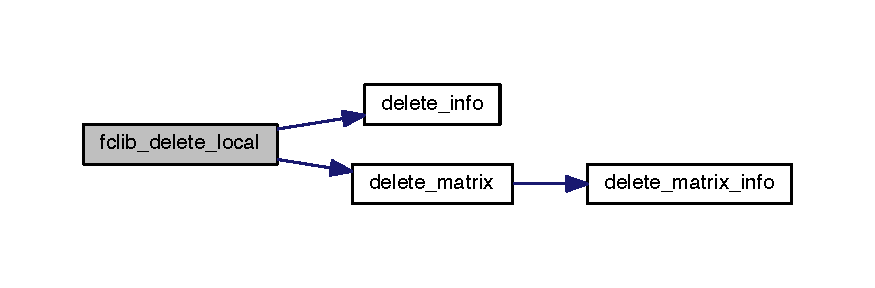
\includegraphics[width=350pt]{fclib_8c_a20292c502d574d412fd8b41aad37225b_cgraph}
\end{center}
\end{figure}


\hypertarget{fclib_8c_a4b70826ccf4a67808e1946036ac6d950}{}\index{fclib.\+c@{fclib.\+c}!fclib\+\_\+delete\+\_\+solutions@{fclib\+\_\+delete\+\_\+solutions}}
\index{fclib\+\_\+delete\+\_\+solutions@{fclib\+\_\+delete\+\_\+solutions}!fclib.\+c@{fclib.\+c}}
\paragraph[{fclib\+\_\+delete\+\_\+solutions(struct fclib\+\_\+solution $\ast$data, int count)}]{\setlength{\rightskip}{0pt plus 5cm}void fclib\+\_\+delete\+\_\+solutions (
\begin{DoxyParamCaption}
\item[{struct {\bf fclib\+\_\+solution} $\ast$}]{data, }
\item[{int}]{count}
\end{DoxyParamCaption}
)}\label{fclib_8c_a4b70826ccf4a67808e1946036ac6d950}


delete solutions or guesses 



Definition at line 854 of file fclib.\+c.



References fclib\+\_\+solution\+::l, fclib\+\_\+solution\+::r, fclib\+\_\+solution\+::u, and fclib\+\_\+solution\+::v.



Referenced by main().


\hypertarget{fclib_8h}{}\subsection{fclib.\+h File Reference}
\label{fclib_8h}\index{fclib.\+h@{fclib.\+h}}
{\ttfamily \#include \char`\"{}csparse.\+h\char`\"{}}\\*
Include dependency graph for fclib.\+h\+:\nopagebreak
\begin{figure}[H]
\begin{center}
\leavevmode
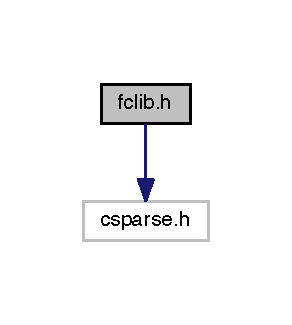
\includegraphics[width=140pt]{fclib_8h__incl}
\end{center}
\end{figure}
This graph shows which files directly or indirectly include this file\+:\nopagebreak
\begin{figure}[H]
\begin{center}
\leavevmode
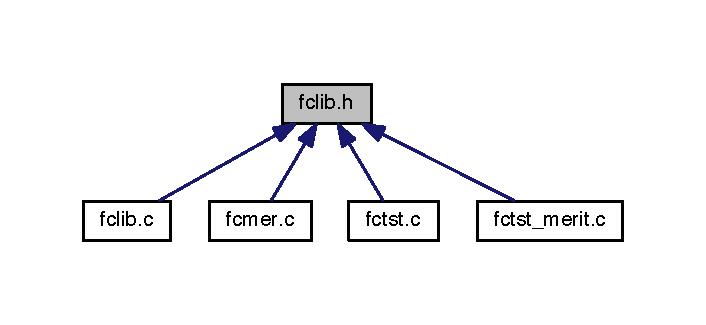
\includegraphics[width=339pt]{fclib_8h__dep__incl}
\end{center}
\end{figure}
\subsubsection*{Classes}
\begin{DoxyCompactItemize}
\item 
struct \hyperlink{structfclib__info}{fclib\+\_\+info}
\begin{DoxyCompactList}\small\item\em This structure allows the user to enter a problem information as a title, a short description and known mathematical properties of the problem. \end{DoxyCompactList}\item 
struct \hyperlink{structfclib__matrix__info}{fclib\+\_\+matrix\+\_\+info}
\begin{DoxyCompactList}\small\item\em This structure allows the user to enter a description for a given matrix (comment, conditionning, determinant, rank.) if they are known. \end{DoxyCompactList}\item 
struct \hyperlink{structfclib__matrix}{fclib\+\_\+matrix}
\begin{DoxyCompactList}\small\item\em matrix in compressed row/column or triplet form \end{DoxyCompactList}\item 
struct \hyperlink{structfclib__global}{fclib\+\_\+global}
\begin{DoxyCompactList}\small\item\em The global frictional contact problem defined by. \end{DoxyCompactList}\item 
struct \hyperlink{structfclib__local}{fclib\+\_\+local}
\begin{DoxyCompactList}\small\item\em The local frictional contact problem defined by. \end{DoxyCompactList}\item 
struct \hyperlink{structfclib__solution}{fclib\+\_\+solution}
\begin{DoxyCompactList}\small\item\em A solution or a guess for the frictional contact problem. \end{DoxyCompactList}\end{DoxyCompactItemize}
\subsubsection*{Enumerations}
\begin{DoxyCompactItemize}
\item 
enum \hyperlink{fclib_8h_a8d23c04ffda9ad1393fc7f3793e4a9a1}{fclib\+\_\+merit} \{ \hyperlink{fclib_8h_a8d23c04ffda9ad1393fc7f3793e4a9a1ada6eeb669c4207de9ebdbc59ab1107b4}{M\+E\+R\+I\+T\+\_\+1}, 
\hyperlink{fclib_8h_a8d23c04ffda9ad1393fc7f3793e4a9a1a907c2eb86a2fff5e525e93538f27fa3a}{M\+E\+R\+I\+T\+\_\+2}
 \}\begin{DoxyCompactList}\small\item\em M\+E\+R\+I\+T\+\_\+1 is a implementation of the merit function based on the natural map for a S\+O\+C\+C\+P. \end{DoxyCompactList}
\end{DoxyCompactItemize}
\subsubsection*{Functions}
\begin{DoxyCompactItemize}
\item 
int \hyperlink{fclib_8h_acd5a38f03c621ce4a53eea28ae6d9e2e}{fclib\+\_\+write\+\_\+global} (struct \hyperlink{structfclib__global}{fclib\+\_\+global} $\ast$problem, const char $\ast$path)
\begin{DoxyCompactList}\small\item\em write global problem; return 1 on success, 0 on failure \end{DoxyCompactList}\item 
int \hyperlink{fclib_8h_a5c4c7bb4d98efc388fdf4a7aa009b87a}{fclib\+\_\+write\+\_\+local} (struct \hyperlink{structfclib__local}{fclib\+\_\+local} $\ast$problem, const char $\ast$path)
\begin{DoxyCompactList}\small\item\em write local problem; return 1 on success, 0 on failure \end{DoxyCompactList}\item 
int \hyperlink{fclib_8h_a6edc26abbeec9f3e9a4fa71e70726988}{fclib\+\_\+write\+\_\+solution} (struct \hyperlink{structfclib__solution}{fclib\+\_\+solution} $\ast$solution, const char $\ast$path)
\begin{DoxyCompactList}\small\item\em write solution; return 1 on success, 0 on failure \end{DoxyCompactList}\item 
int \hyperlink{fclib_8h_a5100104b958b245b883f5d505651a5c1}{fclib\+\_\+write\+\_\+guesses} (int number\+\_\+of\+\_\+guesses, struct \hyperlink{structfclib__solution}{fclib\+\_\+solution} $\ast$guesses, const char $\ast$path)
\begin{DoxyCompactList}\small\item\em write initial guesses; return 1 on success, 0 on failure \end{DoxyCompactList}\item 
struct \hyperlink{structfclib__global}{fclib\+\_\+global} $\ast$ \hyperlink{fclib_8h_a68650a3ef8e5cfca61e10ede3ff59745}{fclib\+\_\+read\+\_\+global} (const char $\ast$path)
\begin{DoxyCompactList}\small\item\em read global problem; return problem on success; N\+U\+L\+L on failure \end{DoxyCompactList}\item 
struct \hyperlink{structfclib__local}{fclib\+\_\+local} $\ast$ \hyperlink{fclib_8h_a1122778ddd33ab84360ec6da584bff99}{fclib\+\_\+read\+\_\+local} (const char $\ast$path)
\begin{DoxyCompactList}\small\item\em read local problem; return problem on success; N\+U\+L\+L on failure \end{DoxyCompactList}\item 
struct \hyperlink{structfclib__solution}{fclib\+\_\+solution} $\ast$ \hyperlink{fclib_8h_a038c74114b0d53fd79785d99cd6c42fb}{fclib\+\_\+read\+\_\+solution} (const char $\ast$path)
\begin{DoxyCompactList}\small\item\em read solution; return solution on success; N\+U\+L\+L on failure \end{DoxyCompactList}\item 
struct \hyperlink{structfclib__solution}{fclib\+\_\+solution} $\ast$ \hyperlink{fclib_8h_ad1392d4746f60eb0030d6f9e80846e53}{fclib\+\_\+read\+\_\+guesses} (const char $\ast$path, int $\ast$number\+\_\+of\+\_\+guesses)
\begin{DoxyCompactList}\small\item\em read initial guesses; return vector of guesses on success; N\+U\+L\+L on failure; output numebr of guesses in the variable pointed by \textquotesingle{}number\+\_\+of\+\_\+guesses\textquotesingle{} \end{DoxyCompactList}\item 
double \hyperlink{fclib_8h_a148e6f5a5567fc5f2961d48f0652f1b9}{fclib\+\_\+merit\+\_\+global} (struct \hyperlink{structfclib__global}{fclib\+\_\+global} $\ast$problem, enum \hyperlink{fclib_8h_a8d23c04ffda9ad1393fc7f3793e4a9a1}{fclib\+\_\+merit} merit, struct \hyperlink{structfclib__solution}{fclib\+\_\+solution} $\ast$solution)
\begin{DoxyCompactList}\small\item\em calculate merit function for a global problem \end{DoxyCompactList}\item 
double \hyperlink{fclib_8h_a60a8a78d06e2ba1a2dc5bce40d49113e}{fclib\+\_\+merit\+\_\+local} (struct \hyperlink{structfclib__local}{fclib\+\_\+local} $\ast$problem, enum \hyperlink{fclib_8h_a8d23c04ffda9ad1393fc7f3793e4a9a1}{fclib\+\_\+merit} merit, struct \hyperlink{structfclib__solution}{fclib\+\_\+solution} $\ast$solution)
\begin{DoxyCompactList}\small\item\em calculate merit function for a local problem \end{DoxyCompactList}\item 
void \hyperlink{fclib_8h_a14b1c35f51633d79f4ed6a680d21d6b4}{fclib\+\_\+delete\+\_\+global} (struct \hyperlink{structfclib__global}{fclib\+\_\+global} $\ast$problem)
\begin{DoxyCompactList}\small\item\em delete global problem \end{DoxyCompactList}\item 
void \hyperlink{fclib_8h_a20292c502d574d412fd8b41aad37225b}{fclib\+\_\+delete\+\_\+local} (struct \hyperlink{structfclib__local}{fclib\+\_\+local} $\ast$problem)
\begin{DoxyCompactList}\small\item\em delete local problem \end{DoxyCompactList}\item 
void \hyperlink{fclib_8h_a4b70826ccf4a67808e1946036ac6d950}{fclib\+\_\+delete\+\_\+solutions} (struct \hyperlink{structfclib__solution}{fclib\+\_\+solution} $\ast$data, int count)
\begin{DoxyCompactList}\small\item\em delete solutions or guesses \end{DoxyCompactList}\item 
int \hyperlink{fclib_8h_a8b3c88579db667d89aa7d7a6c6fd90f4}{fclib\+\_\+create\+\_\+int\+\_\+attributes\+\_\+in\+\_\+info} (const char $\ast$path, const char $\ast$attr\+\_\+name, int attr\+\_\+value)
\begin{DoxyCompactList}\small\item\em create and set attributes of tyoe int in info \end{DoxyCompactList}\end{DoxyCompactItemize}


\subsubsection{Detailed Description}


 \paragraph*{frictional contact library interface }

This C A\+P\+I provides functions to read and write Frictional contact problemes in H\+D\+F5 format Two kind of problem are considered Given 
\begin{DoxyItemize}
\item a symmetric positive semi--definite matrix ${W} \in {\mathrm{I\!R}}^{m \times m} $  
\item a vector $ {q} \in {\mathrm{I\!R}}^m$ 
\item a vector of coefficients of friction $\mu \in{\mathrm{I\!R}}^{n_c}$ 
\end{DoxyItemize}the local F\+C problem is to find two vectors $u\in{\ensuremath{\mathrm{I\!R}}}^m$, the relative local velocity and $r\in {\ensuremath{\mathrm{I\!R}}}^m$, the contact forces denoted by $\mathrm{FC}(W,q,\mu)$ such that \begin{eqnarray*} \begin{cases} \hat u = W r + q +\left[ \left[\begin{array}{c} \mu^\alpha \|u^\alpha_T\|\ \ 0 \ \ 0 \end{array}\right]^T, \alpha = 1 \ldots n_c \right]^T \\ \ \ C^\star_{\mu} \ni {\hat u} \perp r \in C_{\mu} \end{cases} \end{eqnarray*} where the Coulomb friction cone for a contact $\alpha$ is defined by \begin{eqnarray*} \label{eq:CCC} C_{\mu^\alpha}^{\alpha} = \{r^\alpha, \|r^\alpha_T \| \leq \mu^\alpha |r^\alpha_N| \} *\end{eqnarray*} and the set $C^{\alpha,\star}_{\mu^\alpha}$ is its dual. We are also dealing with global F\+C problem defined by Given 
\begin{DoxyItemize}
\item a symmetric positive definite matrix ${M} \in {\mathrm{I\!R}}^{n \times n}$ 
\item a vector $ {f} \in {\mathrm{I\!R}}^n$, 
\item a matrix ${H} \in {\mathrm{I\!R}}^{n \times m}$ 
\item a matrix ${G} \in {\mathrm{I\!R}}^{n \times p}$ 
\item a vector $w \in {\mathrm{I\!R}}^{m}$, 
\item a vector $b \in {\mathrm{I\!R}}^{p}$, 
\item a vector of coefficients of friction $\mu \in {\mathrm{I\!R}}^{n_c}$ 
\end{DoxyItemize}the Global Mixed 3\+D\+F\+C problem is to find four vectors $ {v} \in {\mathrm{I\!R}}^n$, $u\in{\mathrm{I\!R}}^m$, $r\in {\mathrm{I\!R}}^m$ and $\lambda \in {\mathrm{I\!R}}^p$ denoted by $\mathrm{GM3DFC}(M,H,G,w,b,\mu)$ such that \begin{eqnarray*} \begin{cases} M v = {H} {r} + G\lambda + {f} \\ \ \ G^T v +b =0 \\ \ \ \hat u = H^T v + w +\left[ \left[\begin{array}{c} \mu \|u^\alpha_T\|\ \ 0 \ \ 0 \end{array}\right]^T, \alpha = 1 \ldots n_c \right]^T \\ \ \ C^\star_{\mu} \ni {\hat u} \perp r \in C_{\mu} \end{cases} \end{eqnarray*} 

\subsubsection{Enumeration Type Documentation}
\hypertarget{fclib_8h_a8d23c04ffda9ad1393fc7f3793e4a9a1}{}\index{fclib.\+h@{fclib.\+h}!fclib\+\_\+merit@{fclib\+\_\+merit}}
\index{fclib\+\_\+merit@{fclib\+\_\+merit}!fclib.\+h@{fclib.\+h}}
\paragraph[{fclib\+\_\+merit}]{\setlength{\rightskip}{0pt plus 5cm}enum {\bf fclib\+\_\+merit}}\label{fclib_8h_a8d23c04ffda9ad1393fc7f3793e4a9a1}


M\+E\+R\+I\+T\+\_\+1 is a implementation of the merit function based on the natural map for a S\+O\+C\+C\+P. 

\begin{Desc}
\item[Enumerator]\par
\begin{description}
\index{M\+E\+R\+I\+T\+\_\+1@{M\+E\+R\+I\+T\+\_\+1}!fclib.\+h@{fclib.\+h}}\index{fclib.\+h@{fclib.\+h}!M\+E\+R\+I\+T\+\_\+1@{M\+E\+R\+I\+T\+\_\+1}}\item[{\em 
\hypertarget{fclib_8h_a8d23c04ffda9ad1393fc7f3793e4a9a1ada6eeb669c4207de9ebdbc59ab1107b4}{}M\+E\+R\+I\+T\+\_\+1\label{fclib_8h_a8d23c04ffda9ad1393fc7f3793e4a9a1ada6eeb669c4207de9ebdbc59ab1107b4}
}]\index{M\+E\+R\+I\+T\+\_\+2@{M\+E\+R\+I\+T\+\_\+2}!fclib.\+h@{fclib.\+h}}\index{fclib.\+h@{fclib.\+h}!M\+E\+R\+I\+T\+\_\+2@{M\+E\+R\+I\+T\+\_\+2}}\item[{\em 
\hypertarget{fclib_8h_a8d23c04ffda9ad1393fc7f3793e4a9a1a907c2eb86a2fff5e525e93538f27fa3a}{}M\+E\+R\+I\+T\+\_\+2\label{fclib_8h_a8d23c04ffda9ad1393fc7f3793e4a9a1a907c2eb86a2fff5e525e93538f27fa3a}
}]\end{description}
\end{Desc}


Definition at line 269 of file fclib.\+h.



\subsubsection{Function Documentation}
\hypertarget{fclib_8h_acd5a38f03c621ce4a53eea28ae6d9e2e}{}\index{fclib.\+h@{fclib.\+h}!fclib\+\_\+write\+\_\+global@{fclib\+\_\+write\+\_\+global}}
\index{fclib\+\_\+write\+\_\+global@{fclib\+\_\+write\+\_\+global}!fclib.\+h@{fclib.\+h}}
\paragraph[{fclib\+\_\+write\+\_\+global(struct fclib\+\_\+global $\ast$problem, const char $\ast$path)}]{\setlength{\rightskip}{0pt plus 5cm}int fclib\+\_\+write\+\_\+global (
\begin{DoxyParamCaption}
\item[{struct {\bf fclib\+\_\+global} $\ast$}]{problem, }
\item[{const char $\ast$}]{path}
\end{DoxyParamCaption}
)}\label{fclib_8h_acd5a38f03c621ce4a53eea28ae6d9e2e}


write global problem; return 1 on success, 0 on failure 



Definition at line 436 of file fclib.\+c.



References A\+S\+S\+E\+R\+T, fclib\+\_\+global\+::\+G, fclib\+\_\+global\+::\+H, H5\+Gmake(), fclib\+\_\+global\+::info, I\+O, fclib\+\_\+global\+::\+M, fclib\+\_\+global\+::spacedim, write\+\_\+global\+\_\+vectors(), write\+\_\+matrix(), and write\+\_\+problem\+\_\+info().



Referenced by main().



Here is the call graph for this function\+:\nopagebreak
\begin{figure}[H]
\begin{center}
\leavevmode
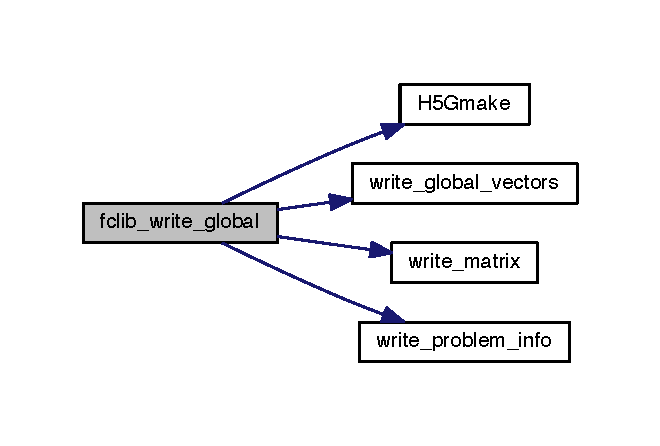
\includegraphics[width=317pt]{fclib_8h_acd5a38f03c621ce4a53eea28ae6d9e2e_cgraph}
\end{center}
\end{figure}


\hypertarget{fclib_8h_a5c4c7bb4d98efc388fdf4a7aa009b87a}{}\index{fclib.\+h@{fclib.\+h}!fclib\+\_\+write\+\_\+local@{fclib\+\_\+write\+\_\+local}}
\index{fclib\+\_\+write\+\_\+local@{fclib\+\_\+write\+\_\+local}!fclib.\+h@{fclib.\+h}}
\paragraph[{fclib\+\_\+write\+\_\+local(struct fclib\+\_\+local $\ast$problem, const char $\ast$path)}]{\setlength{\rightskip}{0pt plus 5cm}int fclib\+\_\+write\+\_\+local (
\begin{DoxyParamCaption}
\item[{struct {\bf fclib\+\_\+local} $\ast$}]{problem, }
\item[{const char $\ast$}]{path}
\end{DoxyParamCaption}
)}\label{fclib_8h_a5c4c7bb4d98efc388fdf4a7aa009b87a}


write local problem; return 1 on success, 0 on failure 



Definition at line 508 of file fclib.\+c.



References A\+S\+S\+E\+R\+T, H5\+Gmake(), fclib\+\_\+local\+::info, I\+O, fclib\+\_\+local\+::\+R, fclib\+\_\+local\+::spacedim, fclib\+\_\+local\+::\+V, fclib\+\_\+local\+::\+W, write\+\_\+local\+\_\+vectors(), write\+\_\+matrix(), and write\+\_\+problem\+\_\+info().



Referenced by main().



Here is the call graph for this function\+:\nopagebreak
\begin{figure}[H]
\begin{center}
\leavevmode
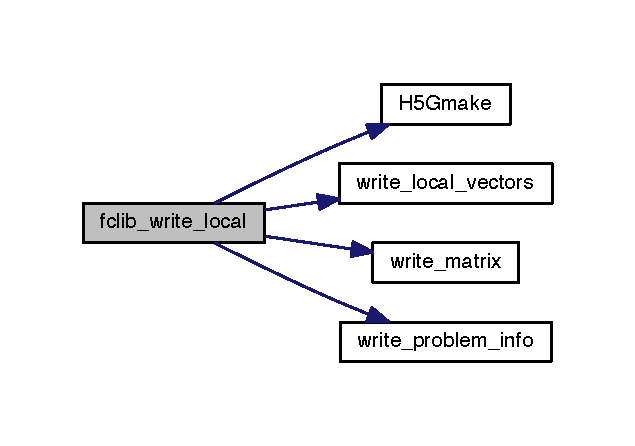
\includegraphics[width=305pt]{fclib_8h_a5c4c7bb4d98efc388fdf4a7aa009b87a_cgraph}
\end{center}
\end{figure}


\hypertarget{fclib_8h_a6edc26abbeec9f3e9a4fa71e70726988}{}\index{fclib.\+h@{fclib.\+h}!fclib\+\_\+write\+\_\+solution@{fclib\+\_\+write\+\_\+solution}}
\index{fclib\+\_\+write\+\_\+solution@{fclib\+\_\+write\+\_\+solution}!fclib.\+h@{fclib.\+h}}
\paragraph[{fclib\+\_\+write\+\_\+solution(struct fclib\+\_\+solution $\ast$solution, const char $\ast$path)}]{\setlength{\rightskip}{0pt plus 5cm}int fclib\+\_\+write\+\_\+solution (
\begin{DoxyParamCaption}
\item[{struct {\bf fclib\+\_\+solution} $\ast$}]{solution, }
\item[{const char $\ast$}]{path}
\end{DoxyParamCaption}
)}\label{fclib_8h_a6edc26abbeec9f3e9a4fa71e70726988}


write solution; return 1 on success, 0 on failure 



Definition at line 576 of file fclib.\+c.



References H5\+Gmake(), I\+O, read\+\_\+nvnunrnl(), and write\+\_\+solution().



Referenced by main().



Here is the call graph for this function\+:\nopagebreak
\begin{figure}[H]
\begin{center}
\leavevmode
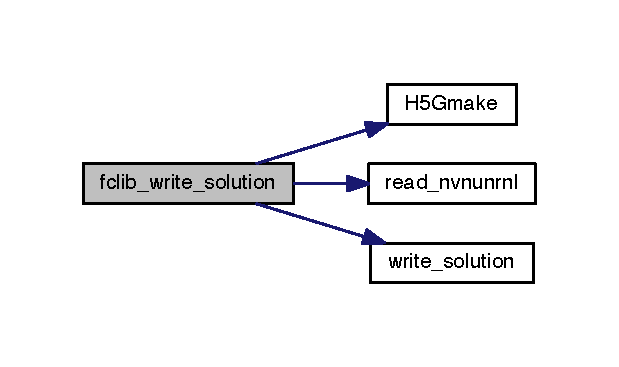
\includegraphics[width=297pt]{fclib_8h_a6edc26abbeec9f3e9a4fa71e70726988_cgraph}
\end{center}
\end{figure}


\hypertarget{fclib_8h_a5100104b958b245b883f5d505651a5c1}{}\index{fclib.\+h@{fclib.\+h}!fclib\+\_\+write\+\_\+guesses@{fclib\+\_\+write\+\_\+guesses}}
\index{fclib\+\_\+write\+\_\+guesses@{fclib\+\_\+write\+\_\+guesses}!fclib.\+h@{fclib.\+h}}
\paragraph[{fclib\+\_\+write\+\_\+guesses(int number\+\_\+of\+\_\+guesses, struct fclib\+\_\+solution $\ast$guesses, const char $\ast$path)}]{\setlength{\rightskip}{0pt plus 5cm}int fclib\+\_\+write\+\_\+guesses (
\begin{DoxyParamCaption}
\item[{int}]{number\+\_\+of\+\_\+guesses, }
\item[{struct {\bf fclib\+\_\+solution} $\ast$}]{guesses, }
\item[{const char $\ast$}]{path}
\end{DoxyParamCaption}
)}\label{fclib_8h_a5100104b958b245b883f5d505651a5c1}


write initial guesses; return 1 on success, 0 on failure 



Definition at line 616 of file fclib.\+c.



References H5\+Gmake(), I\+O, read\+\_\+nvnunrnl(), and write\+\_\+solution().



Referenced by main().



Here is the call graph for this function\+:\nopagebreak
\begin{figure}[H]
\begin{center}
\leavevmode
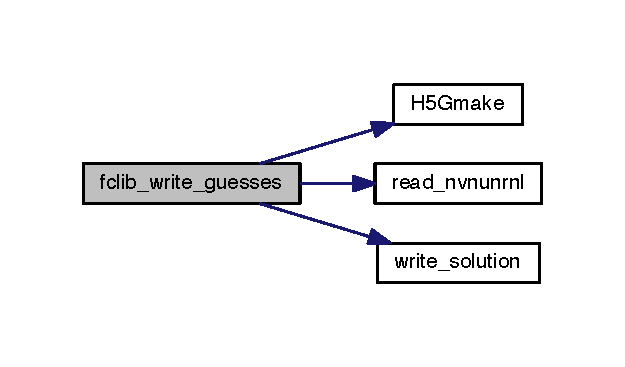
\includegraphics[width=300pt]{fclib_8h_a5100104b958b245b883f5d505651a5c1_cgraph}
\end{center}
\end{figure}


\hypertarget{fclib_8h_a68650a3ef8e5cfca61e10ede3ff59745}{}\index{fclib.\+h@{fclib.\+h}!fclib\+\_\+read\+\_\+global@{fclib\+\_\+read\+\_\+global}}
\index{fclib\+\_\+read\+\_\+global@{fclib\+\_\+read\+\_\+global}!fclib.\+h@{fclib.\+h}}
\paragraph[{fclib\+\_\+read\+\_\+global(const char $\ast$path)}]{\setlength{\rightskip}{0pt plus 5cm}struct {\bf fclib\+\_\+global}$\ast$ fclib\+\_\+read\+\_\+global (
\begin{DoxyParamCaption}
\item[{const char $\ast$}]{path}
\end{DoxyParamCaption}
)}\label{fclib_8h_a68650a3ef8e5cfca61e10ede3ff59745}


read global problem; return problem on success; N\+U\+L\+L on failure 



Definition at line 666 of file fclib.\+c.



References fclib\+\_\+global\+::\+G, fclib\+\_\+global\+::\+H, fclib\+\_\+global\+::info, I\+O, fclib\+\_\+global\+::\+M, M\+M, read\+\_\+global\+\_\+vectors(), read\+\_\+matrix(), read\+\_\+problem\+\_\+info(), and fclib\+\_\+global\+::spacedim.



Referenced by main().



Here is the call graph for this function\+:\nopagebreak
\begin{figure}[H]
\begin{center}
\leavevmode
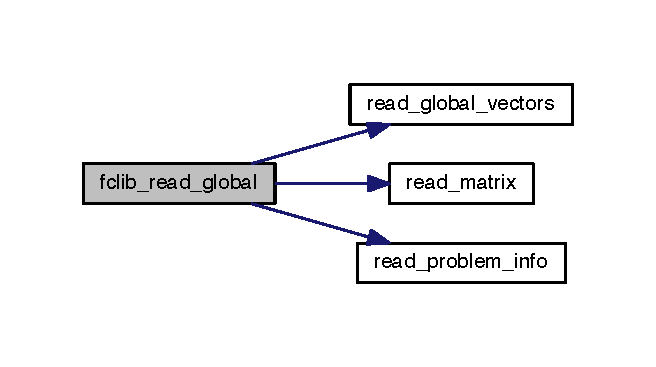
\includegraphics[width=315pt]{fclib_8h_a68650a3ef8e5cfca61e10ede3ff59745_cgraph}
\end{center}
\end{figure}


\hypertarget{fclib_8h_a1122778ddd33ab84360ec6da584bff99}{}\index{fclib.\+h@{fclib.\+h}!fclib\+\_\+read\+\_\+local@{fclib\+\_\+read\+\_\+local}}
\index{fclib\+\_\+read\+\_\+local@{fclib\+\_\+read\+\_\+local}!fclib.\+h@{fclib.\+h}}
\paragraph[{fclib\+\_\+read\+\_\+local(const char $\ast$path)}]{\setlength{\rightskip}{0pt plus 5cm}struct {\bf fclib\+\_\+local}$\ast$ fclib\+\_\+read\+\_\+local (
\begin{DoxyParamCaption}
\item[{const char $\ast$}]{path}
\end{DoxyParamCaption}
)}\label{fclib_8h_a1122778ddd33ab84360ec6da584bff99}


read local problem; return problem on success; N\+U\+L\+L on failure 



Definition at line 716 of file fclib.\+c.



References fclib\+\_\+local\+::info, I\+O, M\+M, fclib\+\_\+local\+::\+R, read\+\_\+local\+\_\+vectors(), read\+\_\+matrix(), read\+\_\+problem\+\_\+info(), fclib\+\_\+local\+::spacedim, fclib\+\_\+local\+::\+V, and fclib\+\_\+local\+::\+W.



Referenced by main().



Here is the call graph for this function\+:\nopagebreak
\begin{figure}[H]
\begin{center}
\leavevmode
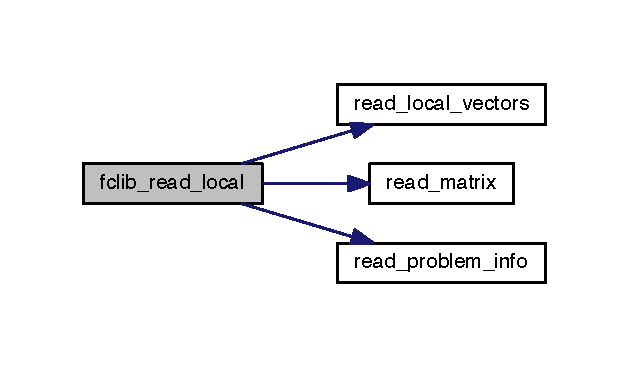
\includegraphics[width=302pt]{fclib_8h_a1122778ddd33ab84360ec6da584bff99_cgraph}
\end{center}
\end{figure}


\hypertarget{fclib_8h_a038c74114b0d53fd79785d99cd6c42fb}{}\index{fclib.\+h@{fclib.\+h}!fclib\+\_\+read\+\_\+solution@{fclib\+\_\+read\+\_\+solution}}
\index{fclib\+\_\+read\+\_\+solution@{fclib\+\_\+read\+\_\+solution}!fclib.\+h@{fclib.\+h}}
\paragraph[{fclib\+\_\+read\+\_\+solution(const char $\ast$path)}]{\setlength{\rightskip}{0pt plus 5cm}struct {\bf fclib\+\_\+solution}$\ast$ fclib\+\_\+read\+\_\+solution (
\begin{DoxyParamCaption}
\item[{const char $\ast$}]{path}
\end{DoxyParamCaption}
)}\label{fclib_8h_a038c74114b0d53fd79785d99cd6c42fb}


read solution; return solution on success; N\+U\+L\+L on failure 



Definition at line 772 of file fclib.\+c.



References I\+O, M\+M, read\+\_\+nvnunrnl(), and read\+\_\+solution().



Referenced by main().



Here is the call graph for this function\+:\nopagebreak
\begin{figure}[H]
\begin{center}
\leavevmode
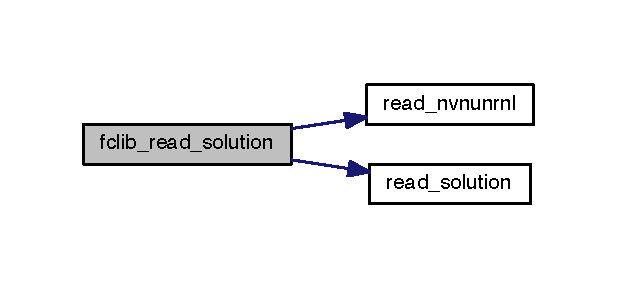
\includegraphics[width=296pt]{fclib_8h_a038c74114b0d53fd79785d99cd6c42fb_cgraph}
\end{center}
\end{figure}


\hypertarget{fclib_8h_ad1392d4746f60eb0030d6f9e80846e53}{}\index{fclib.\+h@{fclib.\+h}!fclib\+\_\+read\+\_\+guesses@{fclib\+\_\+read\+\_\+guesses}}
\index{fclib\+\_\+read\+\_\+guesses@{fclib\+\_\+read\+\_\+guesses}!fclib.\+h@{fclib.\+h}}
\paragraph[{fclib\+\_\+read\+\_\+guesses(const char $\ast$path, int $\ast$number\+\_\+of\+\_\+guesses)}]{\setlength{\rightskip}{0pt plus 5cm}struct {\bf fclib\+\_\+solution}$\ast$ fclib\+\_\+read\+\_\+guesses (
\begin{DoxyParamCaption}
\item[{const char $\ast$}]{path, }
\item[{int $\ast$}]{number\+\_\+of\+\_\+guesses}
\end{DoxyParamCaption}
)}\label{fclib_8h_ad1392d4746f60eb0030d6f9e80846e53}


read initial guesses; return vector of guesses on success; N\+U\+L\+L on failure; output numebr of guesses in the variable pointed by \textquotesingle{}number\+\_\+of\+\_\+guesses\textquotesingle{} 



Definition at line 800 of file fclib.\+c.



References I\+O, M\+M, read\+\_\+nvnunrnl(), and read\+\_\+solution().



Referenced by main().



Here is the call graph for this function\+:\nopagebreak
\begin{figure}[H]
\begin{center}
\leavevmode
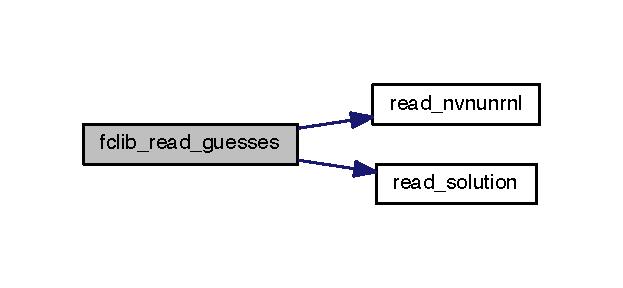
\includegraphics[width=299pt]{fclib_8h_ad1392d4746f60eb0030d6f9e80846e53_cgraph}
\end{center}
\end{figure}


\hypertarget{fclib_8h_a148e6f5a5567fc5f2961d48f0652f1b9}{}\index{fclib.\+h@{fclib.\+h}!fclib\+\_\+merit\+\_\+global@{fclib\+\_\+merit\+\_\+global}}
\index{fclib\+\_\+merit\+\_\+global@{fclib\+\_\+merit\+\_\+global}!fclib.\+h@{fclib.\+h}}
\paragraph[{fclib\+\_\+merit\+\_\+global(struct fclib\+\_\+global $\ast$problem, enum fclib\+\_\+merit merit, struct fclib\+\_\+solution $\ast$solution)}]{\setlength{\rightskip}{0pt plus 5cm}double fclib\+\_\+merit\+\_\+global (
\begin{DoxyParamCaption}
\item[{struct {\bf fclib\+\_\+global} $\ast$}]{problem, }
\item[{enum {\bf fclib\+\_\+merit}}]{merit, }
\item[{struct {\bf fclib\+\_\+solution} $\ast$}]{solution}
\end{DoxyParamCaption}
)}\label{fclib_8h_a148e6f5a5567fc5f2961d48f0652f1b9}


calculate merit function for a global problem 



Definition at line 78 of file fcmer.\+c.



Referenced by main().

\hypertarget{fclib_8h_a60a8a78d06e2ba1a2dc5bce40d49113e}{}\index{fclib.\+h@{fclib.\+h}!fclib\+\_\+merit\+\_\+local@{fclib\+\_\+merit\+\_\+local}}
\index{fclib\+\_\+merit\+\_\+local@{fclib\+\_\+merit\+\_\+local}!fclib.\+h@{fclib.\+h}}
\paragraph[{fclib\+\_\+merit\+\_\+local(struct fclib\+\_\+local $\ast$problem, enum fclib\+\_\+merit merit, struct fclib\+\_\+solution $\ast$solution)}]{\setlength{\rightskip}{0pt plus 5cm}double fclib\+\_\+merit\+\_\+local (
\begin{DoxyParamCaption}
\item[{struct {\bf fclib\+\_\+local} $\ast$}]{problem, }
\item[{enum {\bf fclib\+\_\+merit}}]{merit, }
\item[{struct {\bf fclib\+\_\+solution} $\ast$}]{solution}
\end{DoxyParamCaption}
)}\label{fclib_8h_a60a8a78d06e2ba1a2dc5bce40d49113e}


calculate merit function for a local problem 



Definition at line 84 of file fcmer.\+c.



References dnrm2(), Friction\+Contact3\+D\+\_\+unitary\+\_\+compute\+\_\+and\+\_\+add\+\_\+error(), fclib\+\_\+matrix\+::i, fclib\+\_\+solution\+::l, M\+E\+R\+I\+T\+\_\+1, fclib\+\_\+local\+::mu, fclib\+\_\+matrix\+::n, fclib\+\_\+local\+::q, fclib\+\_\+local\+::\+R, fclib\+\_\+solution\+::r, fclib\+\_\+local\+::s, fclib\+\_\+local\+::spacedim, fclib\+\_\+solution\+::u, fclib\+\_\+local\+::\+V, fclib\+\_\+solution\+::v, and fclib\+\_\+local\+::\+W.



Referenced by main().



Here is the call graph for this function\+:\nopagebreak
\begin{figure}[H]
\begin{center}
\leavevmode
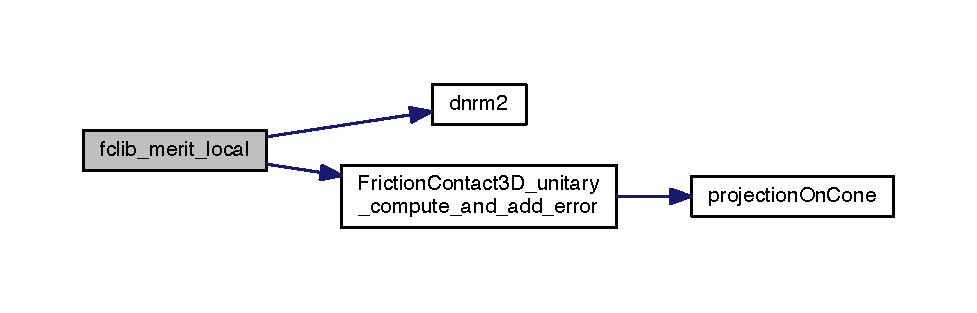
\includegraphics[width=350pt]{fclib_8h_a60a8a78d06e2ba1a2dc5bce40d49113e_cgraph}
\end{center}
\end{figure}


\hypertarget{fclib_8h_a14b1c35f51633d79f4ed6a680d21d6b4}{}\index{fclib.\+h@{fclib.\+h}!fclib\+\_\+delete\+\_\+global@{fclib\+\_\+delete\+\_\+global}}
\index{fclib\+\_\+delete\+\_\+global@{fclib\+\_\+delete\+\_\+global}!fclib.\+h@{fclib.\+h}}
\paragraph[{fclib\+\_\+delete\+\_\+global(struct fclib\+\_\+global $\ast$problem)}]{\setlength{\rightskip}{0pt plus 5cm}void fclib\+\_\+delete\+\_\+global (
\begin{DoxyParamCaption}
\item[{struct {\bf fclib\+\_\+global} $\ast$}]{problem}
\end{DoxyParamCaption}
)}\label{fclib_8h_a14b1c35f51633d79f4ed6a680d21d6b4}


delete global problem 



Definition at line 840 of file fclib.\+c.



References fclib\+\_\+global\+::b, delete\+\_\+info(), delete\+\_\+matrix(), fclib\+\_\+global\+::f, fclib\+\_\+global\+::\+G, fclib\+\_\+global\+::\+H, fclib\+\_\+global\+::info, fclib\+\_\+global\+::\+M, fclib\+\_\+global\+::mu, and fclib\+\_\+global\+::w.



Referenced by main().



Here is the call graph for this function\+:\nopagebreak
\begin{figure}[H]
\begin{center}
\leavevmode
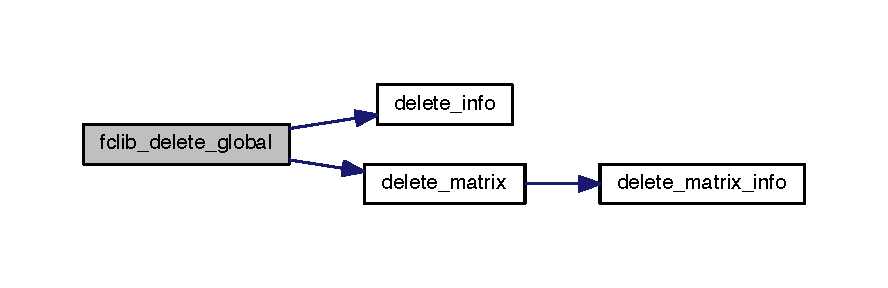
\includegraphics[width=350pt]{fclib_8h_a14b1c35f51633d79f4ed6a680d21d6b4_cgraph}
\end{center}
\end{figure}


\hypertarget{fclib_8h_a20292c502d574d412fd8b41aad37225b}{}\index{fclib.\+h@{fclib.\+h}!fclib\+\_\+delete\+\_\+local@{fclib\+\_\+delete\+\_\+local}}
\index{fclib\+\_\+delete\+\_\+local@{fclib\+\_\+delete\+\_\+local}!fclib.\+h@{fclib.\+h}}
\paragraph[{fclib\+\_\+delete\+\_\+local(struct fclib\+\_\+local $\ast$problem)}]{\setlength{\rightskip}{0pt plus 5cm}void fclib\+\_\+delete\+\_\+local (
\begin{DoxyParamCaption}
\item[{struct {\bf fclib\+\_\+local} $\ast$}]{problem}
\end{DoxyParamCaption}
)}\label{fclib_8h_a20292c502d574d412fd8b41aad37225b}


delete local problem 



Definition at line 853 of file fclib.\+c.



References delete\+\_\+info(), delete\+\_\+matrix(), fclib\+\_\+local\+::info, fclib\+\_\+local\+::mu, fclib\+\_\+local\+::q, fclib\+\_\+local\+::\+R, fclib\+\_\+local\+::s, fclib\+\_\+local\+::\+V, and fclib\+\_\+local\+::\+W.



Referenced by main().



Here is the call graph for this function\+:\nopagebreak
\begin{figure}[H]
\begin{center}
\leavevmode
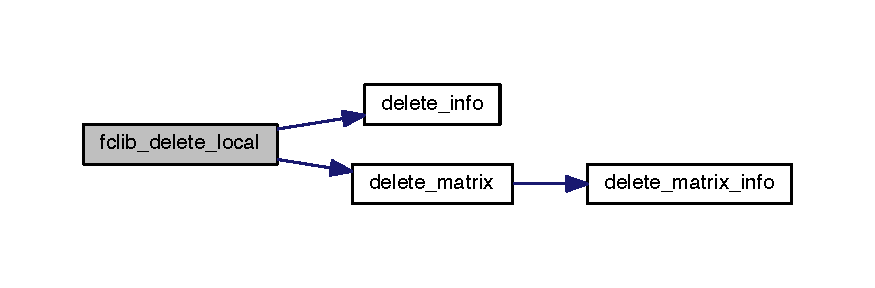
\includegraphics[width=350pt]{fclib_8h_a20292c502d574d412fd8b41aad37225b_cgraph}
\end{center}
\end{figure}


\hypertarget{fclib_8h_a4b70826ccf4a67808e1946036ac6d950}{}\index{fclib.\+h@{fclib.\+h}!fclib\+\_\+delete\+\_\+solutions@{fclib\+\_\+delete\+\_\+solutions}}
\index{fclib\+\_\+delete\+\_\+solutions@{fclib\+\_\+delete\+\_\+solutions}!fclib.\+h@{fclib.\+h}}
\paragraph[{fclib\+\_\+delete\+\_\+solutions(struct fclib\+\_\+solution $\ast$data, int count)}]{\setlength{\rightskip}{0pt plus 5cm}void fclib\+\_\+delete\+\_\+solutions (
\begin{DoxyParamCaption}
\item[{struct {\bf fclib\+\_\+solution} $\ast$}]{data, }
\item[{int}]{count}
\end{DoxyParamCaption}
)}\label{fclib_8h_a4b70826ccf4a67808e1946036ac6d950}


delete solutions or guesses 



Definition at line 865 of file fclib.\+c.



References fclib\+\_\+solution\+::l, fclib\+\_\+solution\+::r, fclib\+\_\+solution\+::u, and fclib\+\_\+solution\+::v.



Referenced by main().

\hypertarget{fclib_8h_a8b3c88579db667d89aa7d7a6c6fd90f4}{}\index{fclib.\+h@{fclib.\+h}!fclib\+\_\+create\+\_\+int\+\_\+attributes\+\_\+in\+\_\+info@{fclib\+\_\+create\+\_\+int\+\_\+attributes\+\_\+in\+\_\+info}}
\index{fclib\+\_\+create\+\_\+int\+\_\+attributes\+\_\+in\+\_\+info@{fclib\+\_\+create\+\_\+int\+\_\+attributes\+\_\+in\+\_\+info}!fclib.\+h@{fclib.\+h}}
\paragraph[{fclib\+\_\+create\+\_\+int\+\_\+attributes\+\_\+in\+\_\+info(const char $\ast$path, const char $\ast$attr\+\_\+name, int attr\+\_\+value)}]{\setlength{\rightskip}{0pt plus 5cm}int fclib\+\_\+create\+\_\+int\+\_\+attributes\+\_\+in\+\_\+info (
\begin{DoxyParamCaption}
\item[{const char $\ast$}]{path, }
\item[{const char $\ast$}]{attr\+\_\+name, }
\item[{int}]{attr\+\_\+value}
\end{DoxyParamCaption}
)}\label{fclib_8h_a8b3c88579db667d89aa7d7a6c6fd90f4}


create and set attributes of tyoe int in info 



Definition at line 387 of file fclib.\+c.



References H5\+Gmake(), and I\+O.



Here is the call graph for this function\+:\nopagebreak
\begin{figure}[H]
\begin{center}
\leavevmode
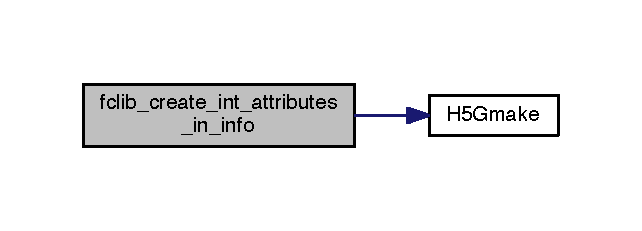
\includegraphics[width=308pt]{fclib_8h_a8b3c88579db667d89aa7d7a6c6fd90f4_cgraph}
\end{center}
\end{figure}



\hypertarget{fcmer_8c}{}\subsection{fcmer.\+c File Reference}
\label{fcmer_8c}\index{fcmer.\+c@{fcmer.\+c}}
{\ttfamily \#include $<$string.\+h$>$}\\*
{\ttfamily \#include $<$stdlib.\+h$>$}\\*
{\ttfamily \#include $<$hdf5.\+h$>$}\\*
{\ttfamily \#include $<$hdf5\+\_\+hl.\+h$>$}\\*
{\ttfamily \#include \char`\"{}fclib.\+h\char`\"{}}\\*
{\ttfamily \#include \char`\"{}fcint.\+h\char`\"{}}\\*
{\ttfamily \#include \char`\"{}math.\+h\char`\"{}}\\*
Include dependency graph for fcmer.\+c\+:\nopagebreak
\begin{figure}[H]
\begin{center}
\leavevmode
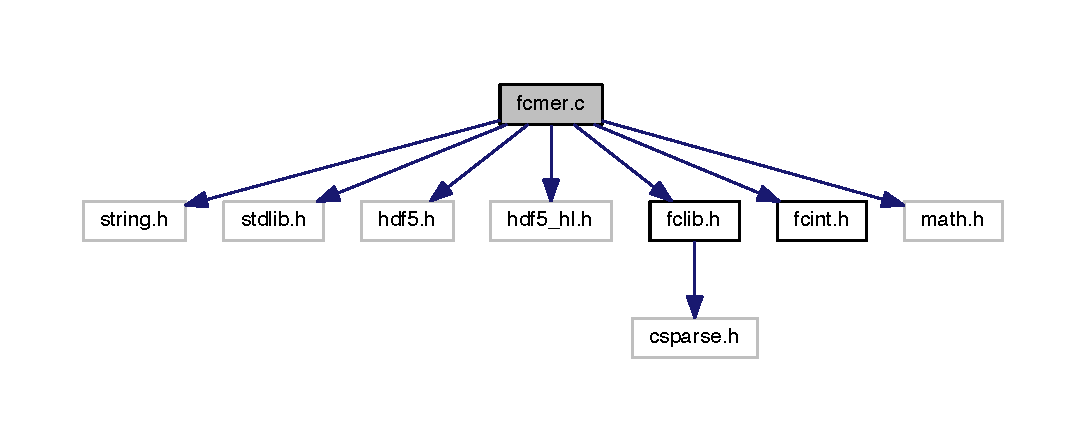
\includegraphics[width=350pt]{fcmer_8c__incl}
\end{center}
\end{figure}
\subsubsection*{Functions}
\begin{DoxyCompactItemize}
\item 
static double \hyperlink{fcmer_8c_a21b2b1a5cdebb20cb283d5409db7f17b}{dnrm2} (double $\ast$v, int n)
\item 
static void \hyperlink{fcmer_8c_a54a7859cadadbf77cbe50743347f33c5}{projection\+On\+Cone} (double $\ast$r, double mu)
\item 
void \hyperlink{fcmer_8c_afee93cccfbaff1232c6083249e1a5e7e}{Friction\+Contact3\+D\+\_\+unitary\+\_\+compute\+\_\+and\+\_\+add\+\_\+error} (double $\ast$z, double $\ast$w, double mu, double $\ast$error)
\item 
double \hyperlink{fcmer_8c_a148e6f5a5567fc5f2961d48f0652f1b9}{fclib\+\_\+merit\+\_\+global} (struct \hyperlink{structfclib__global}{fclib\+\_\+global} $\ast$problem, enum \hyperlink{fclib_8h_a8d23c04ffda9ad1393fc7f3793e4a9a1}{fclib\+\_\+merit} merit, struct \hyperlink{structfclib__solution}{fclib\+\_\+solution} $\ast$solution)
\begin{DoxyCompactList}\small\item\em calculate merit function for a global problem \end{DoxyCompactList}\item 
double \hyperlink{fcmer_8c_a60a8a78d06e2ba1a2dc5bce40d49113e}{fclib\+\_\+merit\+\_\+local} (struct \hyperlink{structfclib__local}{fclib\+\_\+local} $\ast$problem, enum \hyperlink{fclib_8h_a8d23c04ffda9ad1393fc7f3793e4a9a1}{fclib\+\_\+merit} merit, struct \hyperlink{structfclib__solution}{fclib\+\_\+solution} $\ast$solution)
\begin{DoxyCompactList}\small\item\em calculate merit function for a local problem \end{DoxyCompactList}\end{DoxyCompactItemize}


\subsubsection{Function Documentation}
\hypertarget{fcmer_8c_a21b2b1a5cdebb20cb283d5409db7f17b}{}\index{fcmer.\+c@{fcmer.\+c}!dnrm2@{dnrm2}}
\index{dnrm2@{dnrm2}!fcmer.\+c@{fcmer.\+c}}
\paragraph[{dnrm2(double $\ast$v, int n)}]{\setlength{\rightskip}{0pt plus 5cm}static double dnrm2 (
\begin{DoxyParamCaption}
\item[{double $\ast$}]{v, }
\item[{int}]{n}
\end{DoxyParamCaption}
)\hspace{0.3cm}{\ttfamily [inline]}, {\ttfamily [static]}}\label{fcmer_8c_a21b2b1a5cdebb20cb283d5409db7f17b}


Definition at line 27 of file fcmer.\+c.



Referenced by fclib\+\_\+merit\+\_\+local().

\hypertarget{fcmer_8c_a54a7859cadadbf77cbe50743347f33c5}{}\index{fcmer.\+c@{fcmer.\+c}!projection\+On\+Cone@{projection\+On\+Cone}}
\index{projection\+On\+Cone@{projection\+On\+Cone}!fcmer.\+c@{fcmer.\+c}}
\paragraph[{projection\+On\+Cone(double $\ast$r, double mu)}]{\setlength{\rightskip}{0pt plus 5cm}static void projection\+On\+Cone (
\begin{DoxyParamCaption}
\item[{double $\ast$}]{r, }
\item[{double}]{mu}
\end{DoxyParamCaption}
)\hspace{0.3cm}{\ttfamily [inline]}, {\ttfamily [static]}}\label{fcmer_8c_a54a7859cadadbf77cbe50743347f33c5}


Definition at line 35 of file fcmer.\+c.



Referenced by Friction\+Contact3\+D\+\_\+unitary\+\_\+compute\+\_\+and\+\_\+add\+\_\+error().

\hypertarget{fcmer_8c_afee93cccfbaff1232c6083249e1a5e7e}{}\index{fcmer.\+c@{fcmer.\+c}!Friction\+Contact3\+D\+\_\+unitary\+\_\+compute\+\_\+and\+\_\+add\+\_\+error@{Friction\+Contact3\+D\+\_\+unitary\+\_\+compute\+\_\+and\+\_\+add\+\_\+error}}
\index{Friction\+Contact3\+D\+\_\+unitary\+\_\+compute\+\_\+and\+\_\+add\+\_\+error@{Friction\+Contact3\+D\+\_\+unitary\+\_\+compute\+\_\+and\+\_\+add\+\_\+error}!fcmer.\+c@{fcmer.\+c}}
\paragraph[{Friction\+Contact3\+D\+\_\+unitary\+\_\+compute\+\_\+and\+\_\+add\+\_\+error(double $\ast$z, double $\ast$w, double mu, double $\ast$error)}]{\setlength{\rightskip}{0pt plus 5cm}void Friction\+Contact3\+D\+\_\+unitary\+\_\+compute\+\_\+and\+\_\+add\+\_\+error (
\begin{DoxyParamCaption}
\item[{double $\ast$}]{z, }
\item[{double $\ast$}]{w, }
\item[{double}]{mu, }
\item[{double $\ast$}]{error}
\end{DoxyParamCaption}
)}\label{fcmer_8c_afee93cccfbaff1232c6083249e1a5e7e}


Definition at line 59 of file fcmer.\+c.



References projection\+On\+Cone().



Referenced by fclib\+\_\+merit\+\_\+local().



Here is the call graph for this function\+:\nopagebreak
\begin{figure}[H]
\begin{center}
\leavevmode
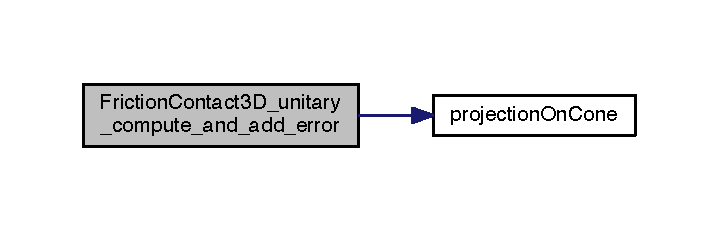
\includegraphics[width=345pt]{fcmer_8c_afee93cccfbaff1232c6083249e1a5e7e_cgraph}
\end{center}
\end{figure}


\hypertarget{fcmer_8c_a148e6f5a5567fc5f2961d48f0652f1b9}{}\index{fcmer.\+c@{fcmer.\+c}!fclib\+\_\+merit\+\_\+global@{fclib\+\_\+merit\+\_\+global}}
\index{fclib\+\_\+merit\+\_\+global@{fclib\+\_\+merit\+\_\+global}!fcmer.\+c@{fcmer.\+c}}
\paragraph[{fclib\+\_\+merit\+\_\+global(struct fclib\+\_\+global $\ast$problem, enum fclib\+\_\+merit merit, struct fclib\+\_\+solution $\ast$solution)}]{\setlength{\rightskip}{0pt plus 5cm}double fclib\+\_\+merit\+\_\+global (
\begin{DoxyParamCaption}
\item[{struct {\bf fclib\+\_\+global} $\ast$}]{problem, }
\item[{enum {\bf fclib\+\_\+merit}}]{merit, }
\item[{struct {\bf fclib\+\_\+solution} $\ast$}]{solution}
\end{DoxyParamCaption}
)}\label{fcmer_8c_a148e6f5a5567fc5f2961d48f0652f1b9}


calculate merit function for a global problem 



Definition at line 78 of file fcmer.\+c.



Referenced by main().

\hypertarget{fcmer_8c_a60a8a78d06e2ba1a2dc5bce40d49113e}{}\index{fcmer.\+c@{fcmer.\+c}!fclib\+\_\+merit\+\_\+local@{fclib\+\_\+merit\+\_\+local}}
\index{fclib\+\_\+merit\+\_\+local@{fclib\+\_\+merit\+\_\+local}!fcmer.\+c@{fcmer.\+c}}
\paragraph[{fclib\+\_\+merit\+\_\+local(struct fclib\+\_\+local $\ast$problem, enum fclib\+\_\+merit merit, struct fclib\+\_\+solution $\ast$solution)}]{\setlength{\rightskip}{0pt plus 5cm}double fclib\+\_\+merit\+\_\+local (
\begin{DoxyParamCaption}
\item[{struct {\bf fclib\+\_\+local} $\ast$}]{problem, }
\item[{enum {\bf fclib\+\_\+merit}}]{merit, }
\item[{struct {\bf fclib\+\_\+solution} $\ast$}]{solution}
\end{DoxyParamCaption}
)}\label{fcmer_8c_a60a8a78d06e2ba1a2dc5bce40d49113e}


calculate merit function for a local problem 



Definition at line 84 of file fcmer.\+c.



References dnrm2(), Friction\+Contact3\+D\+\_\+unitary\+\_\+compute\+\_\+and\+\_\+add\+\_\+error(), fclib\+\_\+matrix\+::i, fclib\+\_\+solution\+::l, M\+E\+R\+I\+T\+\_\+1, fclib\+\_\+local\+::mu, fclib\+\_\+matrix\+::n, fclib\+\_\+local\+::q, fclib\+\_\+local\+::\+R, fclib\+\_\+solution\+::r, fclib\+\_\+local\+::s, fclib\+\_\+local\+::spacedim, fclib\+\_\+solution\+::u, fclib\+\_\+local\+::\+V, fclib\+\_\+solution\+::v, and fclib\+\_\+local\+::\+W.



Referenced by main().



Here is the call graph for this function\+:\nopagebreak
\begin{figure}[H]
\begin{center}
\leavevmode
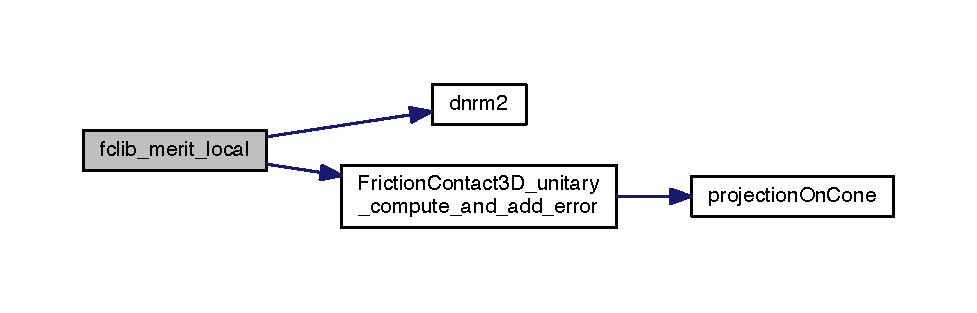
\includegraphics[width=350pt]{fcmer_8c_a60a8a78d06e2ba1a2dc5bce40d49113e_cgraph}
\end{center}
\end{figure}



\hypertarget{fctst_8c}{}\subsection{fctst.\+c File Reference}
\label{fctst_8c}\index{fctst.\+c@{fctst.\+c}}
{\ttfamily \#include $<$string.\+h$>$}\\*
{\ttfamily \#include $<$stdlib.\+h$>$}\\*
{\ttfamily \#include $<$stdio.\+h$>$}\\*
{\ttfamily \#include $<$time.\+h$>$}\\*
{\ttfamily \#include \char`\"{}fclib.\+h\char`\"{}}\\*
{\ttfamily \#include \char`\"{}fcint.\+h\char`\"{}}\\*
Include dependency graph for fctst.\+c\+:\nopagebreak
\begin{figure}[H]
\begin{center}
\leavevmode
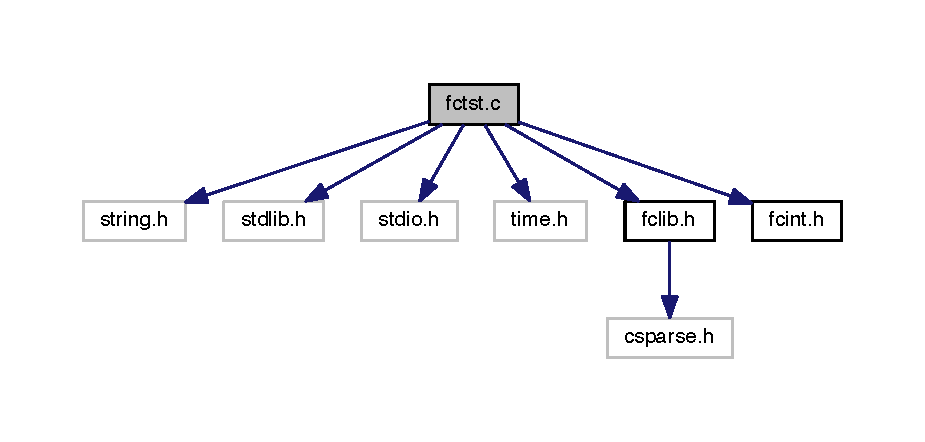
\includegraphics[width=350pt]{fctst_8c__incl}
\end{center}
\end{figure}
\subsubsection*{Functions}
\begin{DoxyCompactItemize}
\item 
static struct \hyperlink{structfclib__matrix__info}{fclib\+\_\+matrix\+\_\+info} $\ast$ \hyperlink{fctst_8c_a5317d629631ea1f011ac56be9ea38b38}{matrix\+\_\+info} (struct \hyperlink{structfclib__matrix}{fclib\+\_\+matrix} $\ast$mat, char $\ast$comment)
\item 
static struct \hyperlink{structfclib__matrix}{fclib\+\_\+matrix} $\ast$ \hyperlink{fctst_8c_a6416171cd1c45fcd483d9f8d72b4d074}{random\+\_\+matrix} (int m, int n)
\item 
static double $\ast$ \hyperlink{fctst_8c_a999ad2a7d7f608315a960fead29ed28b}{random\+\_\+vector} (int n)
\item 
static struct \hyperlink{structfclib__info}{fclib\+\_\+info} $\ast$ \hyperlink{fctst_8c_abacfc09e4ebacd539b34abc2eb6dd26c}{problem\+\_\+info} (char $\ast$title, char $\ast$desc, char $\ast$math)
\item 
static struct \hyperlink{structfclib__global}{fclib\+\_\+global} $\ast$ \hyperlink{fctst_8c_a6bef941fe768030a414543381d847b64}{random\+\_\+global\+\_\+problem} (int global\+\_\+dofs, int contact\+\_\+points, int neq)
\item 
static struct \hyperlink{structfclib__solution}{fclib\+\_\+solution} $\ast$ \hyperlink{fctst_8c_a7aad52ff7bfb95ad106f406bc9c55e58}{random\+\_\+global\+\_\+solutions} (struct \hyperlink{structfclib__global}{fclib\+\_\+global} $\ast$problem, int count)
\item 
static struct \hyperlink{structfclib__local}{fclib\+\_\+local} $\ast$ \hyperlink{fctst_8c_aa112c21ec93e39bb3d3f0461aaa17eec}{random\+\_\+local\+\_\+problem} (int contact\+\_\+points, int neq)
\item 
static struct \hyperlink{structfclib__solution}{fclib\+\_\+solution} $\ast$ \hyperlink{fctst_8c_ab80ee715851eb0c92913d5687498c2d7}{random\+\_\+local\+\_\+solutions} (struct \hyperlink{structfclib__local}{fclib\+\_\+local} $\ast$problem, int count)
\item 
static int \hyperlink{fctst_8c_afe507e5b61471a838e743fe8966e1dde}{compare\+\_\+matrix\+\_\+infos} (struct \hyperlink{structfclib__matrix__info}{fclib\+\_\+matrix\+\_\+info} $\ast$a, struct \hyperlink{structfclib__matrix__info}{fclib\+\_\+matrix\+\_\+info} $\ast$b)
\item 
static int \hyperlink{fctst_8c_ae337371ca0bad878ee90abcb775e94b6}{compare\+\_\+matrices} (char $\ast$name, struct \hyperlink{structfclib__matrix}{fclib\+\_\+matrix} $\ast$a, struct \hyperlink{structfclib__matrix}{fclib\+\_\+matrix} $\ast$b)
\item 
static int \hyperlink{fctst_8c_a67077fe8eef8d36f1bc54695d4e38b07}{compare\+\_\+vectors} (char $\ast$name, int n, double $\ast$a, double $\ast$b)
\item 
static int \hyperlink{fctst_8c_a9616c18dc1480beb7de7875405ba8a69}{compare\+\_\+infos} (struct \hyperlink{structfclib__info}{fclib\+\_\+info} $\ast$a, struct \hyperlink{structfclib__info}{fclib\+\_\+info} $\ast$b)
\item 
static int \hyperlink{fctst_8c_aeadef34f0fb9a9e71e98d044a21fb51f}{compare\+\_\+global\+\_\+problems} (struct \hyperlink{structfclib__global}{fclib\+\_\+global} $\ast$a, struct \hyperlink{structfclib__global}{fclib\+\_\+global} $\ast$b)
\item 
static int \hyperlink{fctst_8c_ab0228efafe00f19b638a3f5cdd03eb98}{compare\+\_\+local\+\_\+problems} (struct \hyperlink{structfclib__local}{fclib\+\_\+local} $\ast$a, struct \hyperlink{structfclib__local}{fclib\+\_\+local} $\ast$b)
\item 
static int \hyperlink{fctst_8c_a65196cbffb155f5d40ff33f2d1b825c2}{compare\+\_\+solutions} (struct \hyperlink{structfclib__solution}{fclib\+\_\+solution} $\ast$a, struct \hyperlink{structfclib__solution}{fclib\+\_\+solution} $\ast$b, int nv, int nr, int nl)
\item 
int \hyperlink{fctst_8c_a3c04138a5bfe5d72780bb7e82a18e627}{main} (int argc, char $\ast$$\ast$argv)
\end{DoxyCompactItemize}


\subsubsection{Function Documentation}
\hypertarget{fctst_8c_a5317d629631ea1f011ac56be9ea38b38}{}\index{fctst.\+c@{fctst.\+c}!matrix\+\_\+info@{matrix\+\_\+info}}
\index{matrix\+\_\+info@{matrix\+\_\+info}!fctst.\+c@{fctst.\+c}}
\paragraph[{matrix\+\_\+info(struct fclib\+\_\+matrix $\ast$mat, char $\ast$comment)}]{\setlength{\rightskip}{0pt plus 5cm}static struct {\bf fclib\+\_\+matrix\+\_\+info}$\ast$ matrix\+\_\+info (
\begin{DoxyParamCaption}
\item[{struct {\bf fclib\+\_\+matrix} $\ast$}]{mat, }
\item[{char $\ast$}]{comment}
\end{DoxyParamCaption}
)\hspace{0.3cm}{\ttfamily [static]}}\label{fctst_8c_a5317d629631ea1f011ac56be9ea38b38}


Definition at line 33 of file fctst.\+c.



References fclib\+\_\+matrix\+\_\+info\+::comment, fclib\+\_\+matrix\+\_\+info\+::conditioning, fclib\+\_\+matrix\+\_\+info\+::determinant, fclib\+\_\+matrix\+::m, M\+M, and fclib\+\_\+matrix\+\_\+info\+::rank.



Referenced by random\+\_\+matrix().

\hypertarget{fctst_8c_a6416171cd1c45fcd483d9f8d72b4d074}{}\index{fctst.\+c@{fctst.\+c}!random\+\_\+matrix@{random\+\_\+matrix}}
\index{random\+\_\+matrix@{random\+\_\+matrix}!fctst.\+c@{fctst.\+c}}
\paragraph[{random\+\_\+matrix(int m, int n)}]{\setlength{\rightskip}{0pt plus 5cm}static struct {\bf fclib\+\_\+matrix}$\ast$ random\+\_\+matrix (
\begin{DoxyParamCaption}
\item[{int}]{m, }
\item[{int}]{n}
\end{DoxyParamCaption}
)\hspace{0.3cm}{\ttfamily [static]}}\label{fctst_8c_a6416171cd1c45fcd483d9f8d72b4d074}


Definition at line 48 of file fctst.\+c.



References fclib\+\_\+matrix\+::i, fclib\+\_\+matrix\+::info, fclib\+\_\+matrix\+::m, matrix\+\_\+info(), M\+M, fclib\+\_\+matrix\+::n, fclib\+\_\+matrix\+::nz, fclib\+\_\+matrix\+::nzmax, fclib\+\_\+matrix\+::p, and fclib\+\_\+matrix\+::x.



Referenced by random\+\_\+global\+\_\+problem(), and random\+\_\+local\+\_\+problem().



Here is the call graph for this function\+:\nopagebreak
\begin{figure}[H]
\begin{center}
\leavevmode
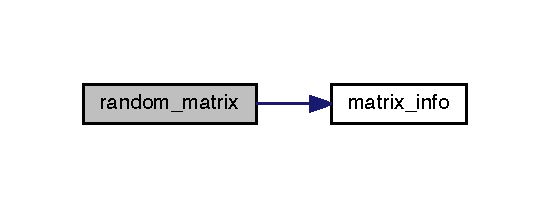
\includegraphics[width=264pt]{fctst_8c_a6416171cd1c45fcd483d9f8d72b4d074_cgraph}
\end{center}
\end{figure}


\hypertarget{fctst_8c_a999ad2a7d7f608315a960fead29ed28b}{}\index{fctst.\+c@{fctst.\+c}!random\+\_\+vector@{random\+\_\+vector}}
\index{random\+\_\+vector@{random\+\_\+vector}!fctst.\+c@{fctst.\+c}}
\paragraph[{random\+\_\+vector(int n)}]{\setlength{\rightskip}{0pt plus 5cm}static double$\ast$ random\+\_\+vector (
\begin{DoxyParamCaption}
\item[{int}]{n}
\end{DoxyParamCaption}
)\hspace{0.3cm}{\ttfamily [static]}}\label{fctst_8c_a999ad2a7d7f608315a960fead29ed28b}


Definition at line 91 of file fctst.\+c.



References M\+M.



Referenced by random\+\_\+global\+\_\+problem(), random\+\_\+global\+\_\+solutions(), random\+\_\+local\+\_\+problem(), and random\+\_\+local\+\_\+solutions().

\hypertarget{fctst_8c_abacfc09e4ebacd539b34abc2eb6dd26c}{}\index{fctst.\+c@{fctst.\+c}!problem\+\_\+info@{problem\+\_\+info}}
\index{problem\+\_\+info@{problem\+\_\+info}!fctst.\+c@{fctst.\+c}}
\paragraph[{problem\+\_\+info(char $\ast$title, char $\ast$desc, char $\ast$math)}]{\setlength{\rightskip}{0pt plus 5cm}static struct {\bf fclib\+\_\+info}$\ast$ problem\+\_\+info (
\begin{DoxyParamCaption}
\item[{char $\ast$}]{title, }
\item[{char $\ast$}]{desc, }
\item[{char $\ast$}]{math}
\end{DoxyParamCaption}
)\hspace{0.3cm}{\ttfamily [static]}}\label{fctst_8c_abacfc09e4ebacd539b34abc2eb6dd26c}


Definition at line 102 of file fctst.\+c.



References fclib\+\_\+info\+::description, fclib\+\_\+info\+::math\+\_\+info, M\+M, and fclib\+\_\+info\+::title.



Referenced by random\+\_\+global\+\_\+problem(), and random\+\_\+local\+\_\+problem().

\hypertarget{fctst_8c_a6bef941fe768030a414543381d847b64}{}\index{fctst.\+c@{fctst.\+c}!random\+\_\+global\+\_\+problem@{random\+\_\+global\+\_\+problem}}
\index{random\+\_\+global\+\_\+problem@{random\+\_\+global\+\_\+problem}!fctst.\+c@{fctst.\+c}}
\paragraph[{random\+\_\+global\+\_\+problem(int global\+\_\+dofs, int contact\+\_\+points, int neq)}]{\setlength{\rightskip}{0pt plus 5cm}static struct {\bf fclib\+\_\+global}$\ast$ random\+\_\+global\+\_\+problem (
\begin{DoxyParamCaption}
\item[{int}]{global\+\_\+dofs, }
\item[{int}]{contact\+\_\+points, }
\item[{int}]{neq}
\end{DoxyParamCaption}
)\hspace{0.3cm}{\ttfamily [static]}}\label{fctst_8c_a6bef941fe768030a414543381d847b64}


Definition at line 118 of file fctst.\+c.



References fclib\+\_\+global\+::b, fclib\+\_\+global\+::f, fclib\+\_\+global\+::\+G, fclib\+\_\+global\+::\+H, fclib\+\_\+global\+::info, fclib\+\_\+global\+::\+M, M\+M, fclib\+\_\+global\+::mu, fclib\+\_\+matrix\+::n, problem\+\_\+info(), random\+\_\+matrix(), random\+\_\+vector(), fclib\+\_\+global\+::spacedim, and fclib\+\_\+global\+::w.



Referenced by main().



Here is the call graph for this function\+:\nopagebreak
\begin{figure}[H]
\begin{center}
\leavevmode
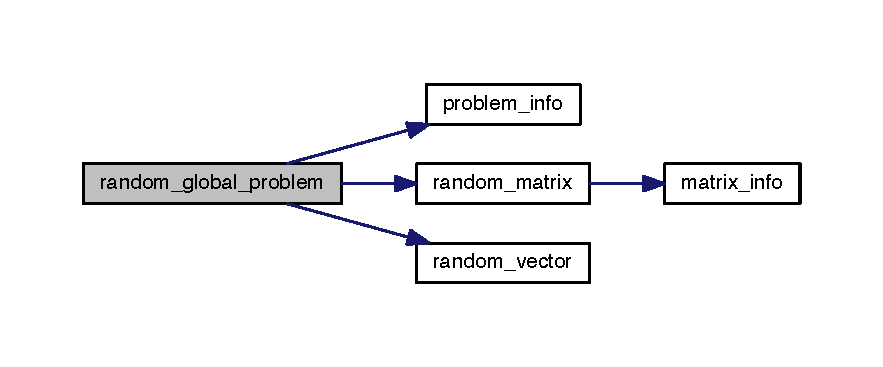
\includegraphics[width=350pt]{fctst_8c_a6bef941fe768030a414543381d847b64_cgraph}
\end{center}
\end{figure}


\hypertarget{fctst_8c_a7aad52ff7bfb95ad106f406bc9c55e58}{}\index{fctst.\+c@{fctst.\+c}!random\+\_\+global\+\_\+solutions@{random\+\_\+global\+\_\+solutions}}
\index{random\+\_\+global\+\_\+solutions@{random\+\_\+global\+\_\+solutions}!fctst.\+c@{fctst.\+c}}
\paragraph[{random\+\_\+global\+\_\+solutions(struct fclib\+\_\+global $\ast$problem, int count)}]{\setlength{\rightskip}{0pt plus 5cm}static struct {\bf fclib\+\_\+solution}$\ast$ random\+\_\+global\+\_\+solutions (
\begin{DoxyParamCaption}
\item[{struct {\bf fclib\+\_\+global} $\ast$}]{problem, }
\item[{int}]{count}
\end{DoxyParamCaption}
)\hspace{0.3cm}{\ttfamily [static]}}\label{fctst_8c_a7aad52ff7bfb95ad106f406bc9c55e58}


Definition at line 141 of file fctst.\+c.



References fclib\+\_\+global\+::\+G, fclib\+\_\+global\+::\+H, fclib\+\_\+solution\+::l, fclib\+\_\+global\+::\+M, M\+M, fclib\+\_\+matrix\+::n, fclib\+\_\+solution\+::r, random\+\_\+vector(), fclib\+\_\+solution\+::u, and fclib\+\_\+solution\+::v.



Referenced by main().



Here is the call graph for this function\+:\nopagebreak
\begin{figure}[H]
\begin{center}
\leavevmode
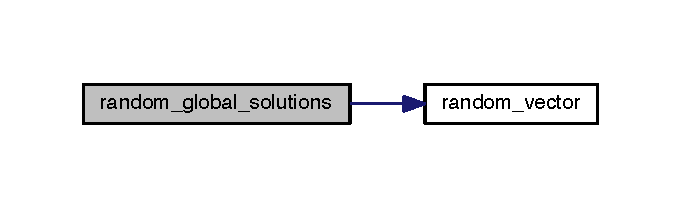
\includegraphics[width=327pt]{fctst_8c_a7aad52ff7bfb95ad106f406bc9c55e58_cgraph}
\end{center}
\end{figure}


\hypertarget{fctst_8c_aa112c21ec93e39bb3d3f0461aaa17eec}{}\index{fctst.\+c@{fctst.\+c}!random\+\_\+local\+\_\+problem@{random\+\_\+local\+\_\+problem}}
\index{random\+\_\+local\+\_\+problem@{random\+\_\+local\+\_\+problem}!fctst.\+c@{fctst.\+c}}
\paragraph[{random\+\_\+local\+\_\+problem(int contact\+\_\+points, int neq)}]{\setlength{\rightskip}{0pt plus 5cm}static struct {\bf fclib\+\_\+local}$\ast$ random\+\_\+local\+\_\+problem (
\begin{DoxyParamCaption}
\item[{int}]{contact\+\_\+points, }
\item[{int}]{neq}
\end{DoxyParamCaption}
)\hspace{0.3cm}{\ttfamily [static]}}\label{fctst_8c_aa112c21ec93e39bb3d3f0461aaa17eec}


Definition at line 161 of file fctst.\+c.



References fclib\+\_\+local\+::info, M\+M, fclib\+\_\+local\+::mu, problem\+\_\+info(), fclib\+\_\+local\+::q, fclib\+\_\+local\+::\+R, random\+\_\+matrix(), random\+\_\+vector(), fclib\+\_\+local\+::s, fclib\+\_\+local\+::spacedim, fclib\+\_\+local\+::\+V, and fclib\+\_\+local\+::\+W.



Referenced by main().



Here is the call graph for this function\+:\nopagebreak
\begin{figure}[H]
\begin{center}
\leavevmode
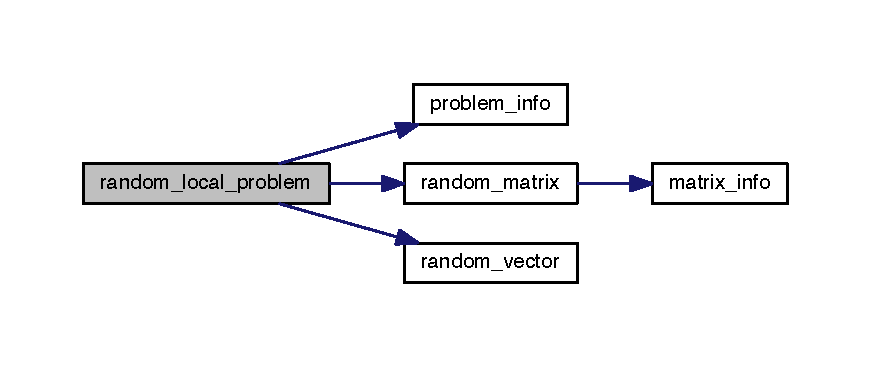
\includegraphics[width=350pt]{fctst_8c_aa112c21ec93e39bb3d3f0461aaa17eec_cgraph}
\end{center}
\end{figure}


\hypertarget{fctst_8c_ab80ee715851eb0c92913d5687498c2d7}{}\index{fctst.\+c@{fctst.\+c}!random\+\_\+local\+\_\+solutions@{random\+\_\+local\+\_\+solutions}}
\index{random\+\_\+local\+\_\+solutions@{random\+\_\+local\+\_\+solutions}!fctst.\+c@{fctst.\+c}}
\paragraph[{random\+\_\+local\+\_\+solutions(struct fclib\+\_\+local $\ast$problem, int count)}]{\setlength{\rightskip}{0pt plus 5cm}static struct {\bf fclib\+\_\+solution}$\ast$ random\+\_\+local\+\_\+solutions (
\begin{DoxyParamCaption}
\item[{struct {\bf fclib\+\_\+local} $\ast$}]{problem, }
\item[{int}]{count}
\end{DoxyParamCaption}
)\hspace{0.3cm}{\ttfamily [static]}}\label{fctst_8c_ab80ee715851eb0c92913d5687498c2d7}


Definition at line 189 of file fctst.\+c.



References fclib\+\_\+solution\+::l, M\+M, fclib\+\_\+matrix\+::n, fclib\+\_\+local\+::\+R, fclib\+\_\+solution\+::r, random\+\_\+vector(), fclib\+\_\+solution\+::u, fclib\+\_\+solution\+::v, and fclib\+\_\+local\+::\+W.



Referenced by main().



Here is the call graph for this function\+:\nopagebreak
\begin{figure}[H]
\begin{center}
\leavevmode
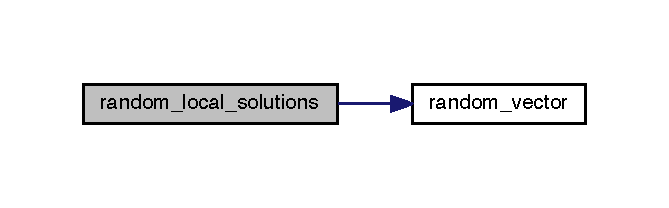
\includegraphics[width=321pt]{fctst_8c_ab80ee715851eb0c92913d5687498c2d7_cgraph}
\end{center}
\end{figure}


\hypertarget{fctst_8c_afe507e5b61471a838e743fe8966e1dde}{}\index{fctst.\+c@{fctst.\+c}!compare\+\_\+matrix\+\_\+infos@{compare\+\_\+matrix\+\_\+infos}}
\index{compare\+\_\+matrix\+\_\+infos@{compare\+\_\+matrix\+\_\+infos}!fctst.\+c@{fctst.\+c}}
\paragraph[{compare\+\_\+matrix\+\_\+infos(struct fclib\+\_\+matrix\+\_\+info $\ast$a, struct fclib\+\_\+matrix\+\_\+info $\ast$b)}]{\setlength{\rightskip}{0pt plus 5cm}static int compare\+\_\+matrix\+\_\+infos (
\begin{DoxyParamCaption}
\item[{struct {\bf fclib\+\_\+matrix\+\_\+info} $\ast$}]{a, }
\item[{struct {\bf fclib\+\_\+matrix\+\_\+info} $\ast$}]{b}
\end{DoxyParamCaption}
)\hspace{0.3cm}{\ttfamily [static]}}\label{fctst_8c_afe507e5b61471a838e743fe8966e1dde}


Definition at line 209 of file fctst.\+c.



References fclib\+\_\+matrix\+\_\+info\+::comment, fclib\+\_\+matrix\+\_\+info\+::conditioning, fclib\+\_\+matrix\+\_\+info\+::determinant, and fclib\+\_\+matrix\+\_\+info\+::rank.



Referenced by compare\+\_\+matrices().

\hypertarget{fctst_8c_ae337371ca0bad878ee90abcb775e94b6}{}\index{fctst.\+c@{fctst.\+c}!compare\+\_\+matrices@{compare\+\_\+matrices}}
\index{compare\+\_\+matrices@{compare\+\_\+matrices}!fctst.\+c@{fctst.\+c}}
\paragraph[{compare\+\_\+matrices(char $\ast$name, struct fclib\+\_\+matrix $\ast$a, struct fclib\+\_\+matrix $\ast$b)}]{\setlength{\rightskip}{0pt plus 5cm}static int compare\+\_\+matrices (
\begin{DoxyParamCaption}
\item[{char $\ast$}]{name, }
\item[{struct {\bf fclib\+\_\+matrix} $\ast$}]{a, }
\item[{struct {\bf fclib\+\_\+matrix} $\ast$}]{b}
\end{DoxyParamCaption}
)\hspace{0.3cm}{\ttfamily [static]}}\label{fctst_8c_ae337371ca0bad878ee90abcb775e94b6}


Definition at line 222 of file fctst.\+c.



References compare\+\_\+matrix\+\_\+infos(), fclib\+\_\+matrix\+::i, fclib\+\_\+matrix\+::info, fclib\+\_\+matrix\+::m, fclib\+\_\+matrix\+::n, fclib\+\_\+matrix\+::nz, fclib\+\_\+matrix\+::nzmax, fclib\+\_\+matrix\+::p, and fclib\+\_\+matrix\+::x.



Referenced by compare\+\_\+global\+\_\+problems(), and compare\+\_\+local\+\_\+problems().



Here is the call graph for this function\+:\nopagebreak
\begin{figure}[H]
\begin{center}
\leavevmode
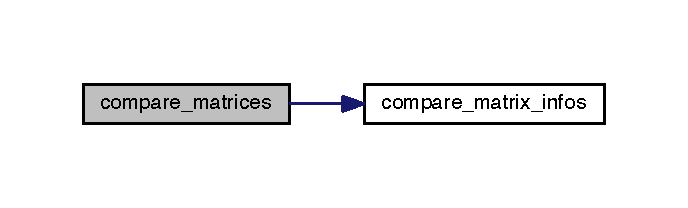
\includegraphics[width=330pt]{fctst_8c_ae337371ca0bad878ee90abcb775e94b6_cgraph}
\end{center}
\end{figure}


\hypertarget{fctst_8c_a67077fe8eef8d36f1bc54695d4e38b07}{}\index{fctst.\+c@{fctst.\+c}!compare\+\_\+vectors@{compare\+\_\+vectors}}
\index{compare\+\_\+vectors@{compare\+\_\+vectors}!fctst.\+c@{fctst.\+c}}
\paragraph[{compare\+\_\+vectors(char $\ast$name, int n, double $\ast$a, double $\ast$b)}]{\setlength{\rightskip}{0pt plus 5cm}static int compare\+\_\+vectors (
\begin{DoxyParamCaption}
\item[{char $\ast$}]{name, }
\item[{int}]{n, }
\item[{double $\ast$}]{a, }
\item[{double $\ast$}]{b}
\end{DoxyParamCaption}
)\hspace{0.3cm}{\ttfamily [static]}}\label{fctst_8c_a67077fe8eef8d36f1bc54695d4e38b07}


Definition at line 327 of file fctst.\+c.



Referenced by compare\+\_\+global\+\_\+problems(), compare\+\_\+local\+\_\+problems(), and compare\+\_\+solutions().

\hypertarget{fctst_8c_a9616c18dc1480beb7de7875405ba8a69}{}\index{fctst.\+c@{fctst.\+c}!compare\+\_\+infos@{compare\+\_\+infos}}
\index{compare\+\_\+infos@{compare\+\_\+infos}!fctst.\+c@{fctst.\+c}}
\paragraph[{compare\+\_\+infos(struct fclib\+\_\+info $\ast$a, struct fclib\+\_\+info $\ast$b)}]{\setlength{\rightskip}{0pt plus 5cm}static int compare\+\_\+infos (
\begin{DoxyParamCaption}
\item[{struct {\bf fclib\+\_\+info} $\ast$}]{a, }
\item[{struct {\bf fclib\+\_\+info} $\ast$}]{b}
\end{DoxyParamCaption}
)\hspace{0.3cm}{\ttfamily [static]}}\label{fctst_8c_a9616c18dc1480beb7de7875405ba8a69}


Definition at line 347 of file fctst.\+c.



References fclib\+\_\+info\+::description, fclib\+\_\+info\+::math\+\_\+info, and fclib\+\_\+info\+::title.



Referenced by compare\+\_\+global\+\_\+problems(), and compare\+\_\+local\+\_\+problems().

\hypertarget{fctst_8c_aeadef34f0fb9a9e71e98d044a21fb51f}{}\index{fctst.\+c@{fctst.\+c}!compare\+\_\+global\+\_\+problems@{compare\+\_\+global\+\_\+problems}}
\index{compare\+\_\+global\+\_\+problems@{compare\+\_\+global\+\_\+problems}!fctst.\+c@{fctst.\+c}}
\paragraph[{compare\+\_\+global\+\_\+problems(struct fclib\+\_\+global $\ast$a, struct fclib\+\_\+global $\ast$b)}]{\setlength{\rightskip}{0pt plus 5cm}static int compare\+\_\+global\+\_\+problems (
\begin{DoxyParamCaption}
\item[{struct {\bf fclib\+\_\+global} $\ast$}]{a, }
\item[{struct {\bf fclib\+\_\+global} $\ast$}]{b}
\end{DoxyParamCaption}
)\hspace{0.3cm}{\ttfamily [static]}}\label{fctst_8c_aeadef34f0fb9a9e71e98d044a21fb51f}


Definition at line 359 of file fctst.\+c.



References fclib\+\_\+global\+::b, compare\+\_\+infos(), compare\+\_\+matrices(), compare\+\_\+vectors(), fclib\+\_\+global\+::f, fclib\+\_\+global\+::\+G, fclib\+\_\+global\+::\+H, fclib\+\_\+global\+::info, fclib\+\_\+matrix\+::m, fclib\+\_\+global\+::\+M, fclib\+\_\+global\+::mu, fclib\+\_\+matrix\+::n, fclib\+\_\+global\+::spacedim, and fclib\+\_\+global\+::w.



Referenced by main().



Here is the call graph for this function\+:\nopagebreak
\begin{figure}[H]
\begin{center}
\leavevmode
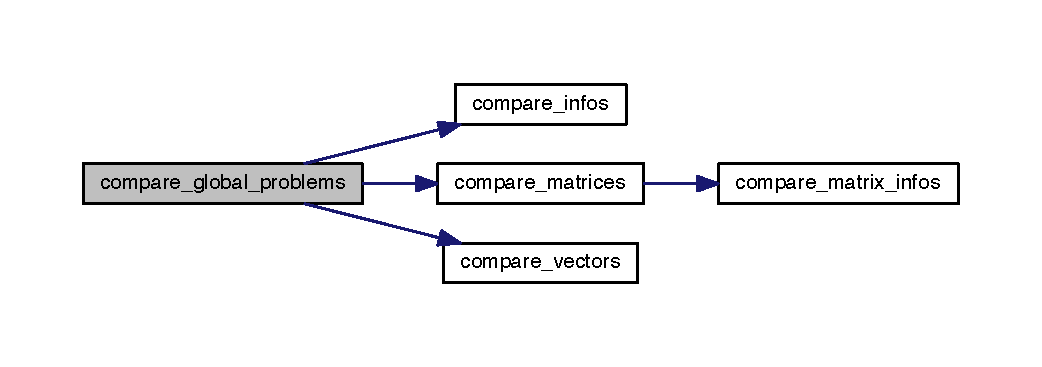
\includegraphics[width=350pt]{fctst_8c_aeadef34f0fb9a9e71e98d044a21fb51f_cgraph}
\end{center}
\end{figure}


\hypertarget{fctst_8c_ab0228efafe00f19b638a3f5cdd03eb98}{}\index{fctst.\+c@{fctst.\+c}!compare\+\_\+local\+\_\+problems@{compare\+\_\+local\+\_\+problems}}
\index{compare\+\_\+local\+\_\+problems@{compare\+\_\+local\+\_\+problems}!fctst.\+c@{fctst.\+c}}
\paragraph[{compare\+\_\+local\+\_\+problems(struct fclib\+\_\+local $\ast$a, struct fclib\+\_\+local $\ast$b)}]{\setlength{\rightskip}{0pt plus 5cm}static int compare\+\_\+local\+\_\+problems (
\begin{DoxyParamCaption}
\item[{struct {\bf fclib\+\_\+local} $\ast$}]{a, }
\item[{struct {\bf fclib\+\_\+local} $\ast$}]{b}
\end{DoxyParamCaption}
)\hspace{0.3cm}{\ttfamily [static]}}\label{fctst_8c_ab0228efafe00f19b638a3f5cdd03eb98}


Definition at line 375 of file fctst.\+c.



References compare\+\_\+infos(), compare\+\_\+matrices(), compare\+\_\+vectors(), fclib\+\_\+local\+::info, fclib\+\_\+local\+::mu, fclib\+\_\+matrix\+::n, fclib\+\_\+local\+::q, fclib\+\_\+local\+::\+R, fclib\+\_\+local\+::s, fclib\+\_\+local\+::spacedim, fclib\+\_\+local\+::\+V, and fclib\+\_\+local\+::\+W.



Referenced by main().



Here is the call graph for this function\+:\nopagebreak
\begin{figure}[H]
\begin{center}
\leavevmode
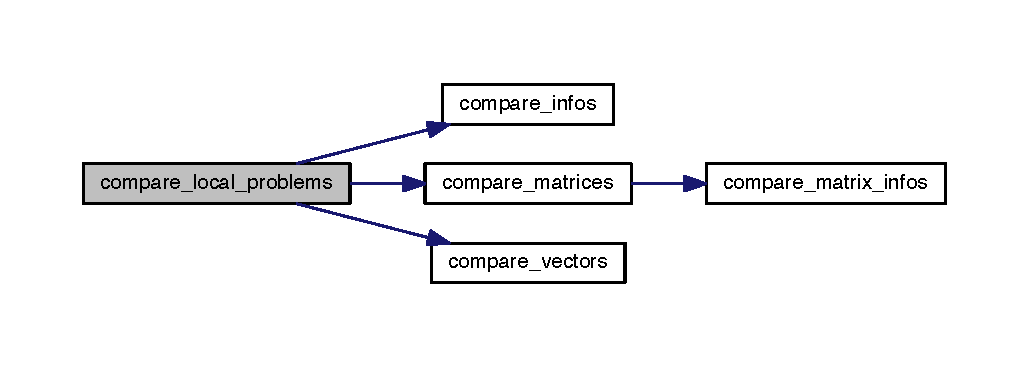
\includegraphics[width=350pt]{fctst_8c_ab0228efafe00f19b638a3f5cdd03eb98_cgraph}
\end{center}
\end{figure}


\hypertarget{fctst_8c_a65196cbffb155f5d40ff33f2d1b825c2}{}\index{fctst.\+c@{fctst.\+c}!compare\+\_\+solutions@{compare\+\_\+solutions}}
\index{compare\+\_\+solutions@{compare\+\_\+solutions}!fctst.\+c@{fctst.\+c}}
\paragraph[{compare\+\_\+solutions(struct fclib\+\_\+solution $\ast$a, struct fclib\+\_\+solution $\ast$b, int nv, int nr, int nl)}]{\setlength{\rightskip}{0pt plus 5cm}static int compare\+\_\+solutions (
\begin{DoxyParamCaption}
\item[{struct {\bf fclib\+\_\+solution} $\ast$}]{a, }
\item[{struct {\bf fclib\+\_\+solution} $\ast$}]{b, }
\item[{int}]{nv, }
\item[{int}]{nr, }
\item[{int}]{nl}
\end{DoxyParamCaption}
)\hspace{0.3cm}{\ttfamily [static]}}\label{fctst_8c_a65196cbffb155f5d40ff33f2d1b825c2}


Definition at line 390 of file fctst.\+c.



References compare\+\_\+vectors(), fclib\+\_\+solution\+::l, fclib\+\_\+solution\+::r, fclib\+\_\+solution\+::u, and fclib\+\_\+solution\+::v.



Referenced by main().



Here is the call graph for this function\+:\nopagebreak
\begin{figure}[H]
\begin{center}
\leavevmode
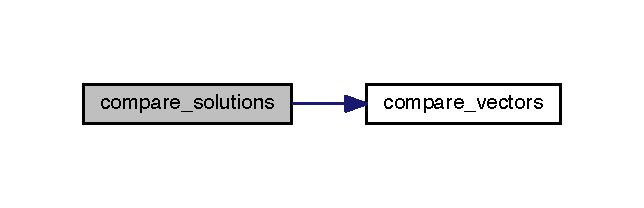
\includegraphics[width=309pt]{fctst_8c_a65196cbffb155f5d40ff33f2d1b825c2_cgraph}
\end{center}
\end{figure}


\hypertarget{fctst_8c_a3c04138a5bfe5d72780bb7e82a18e627}{}\index{fctst.\+c@{fctst.\+c}!main@{main}}
\index{main@{main}!fctst.\+c@{fctst.\+c}}
\paragraph[{main(int argc, char $\ast$$\ast$argv)}]{\setlength{\rightskip}{0pt plus 5cm}int main (
\begin{DoxyParamCaption}
\item[{int}]{argc, }
\item[{char $\ast$$\ast$}]{argv}
\end{DoxyParamCaption}
)}\label{fctst_8c_a3c04138a5bfe5d72780bb7e82a18e627}


Definition at line 400 of file fctst.\+c.



References A\+S\+S\+E\+R\+T, compare\+\_\+global\+\_\+problems(), compare\+\_\+local\+\_\+problems(), compare\+\_\+solutions(), fclib\+\_\+delete\+\_\+global(), fclib\+\_\+delete\+\_\+local(), fclib\+\_\+delete\+\_\+solutions(), fclib\+\_\+merit\+\_\+local(), fclib\+\_\+read\+\_\+global(), fclib\+\_\+read\+\_\+guesses(), fclib\+\_\+read\+\_\+local(), fclib\+\_\+read\+\_\+solution(), fclib\+\_\+write\+\_\+global(), fclib\+\_\+write\+\_\+guesses(), fclib\+\_\+write\+\_\+local(), fclib\+\_\+write\+\_\+solution(), fclib\+\_\+global\+::\+G, fclib\+\_\+global\+::\+H, fclib\+\_\+matrix\+::m, fclib\+\_\+global\+::\+M, M\+E\+R\+I\+T\+\_\+1, fclib\+\_\+matrix\+::n, fclib\+\_\+local\+::\+R, random\+\_\+global\+\_\+problem(), random\+\_\+global\+\_\+solutions(), random\+\_\+local\+\_\+problem(), random\+\_\+local\+\_\+solutions(), and fclib\+\_\+local\+::\+W.



Here is the call graph for this function\+:\nopagebreak
\begin{figure}[H]
\begin{center}
\leavevmode
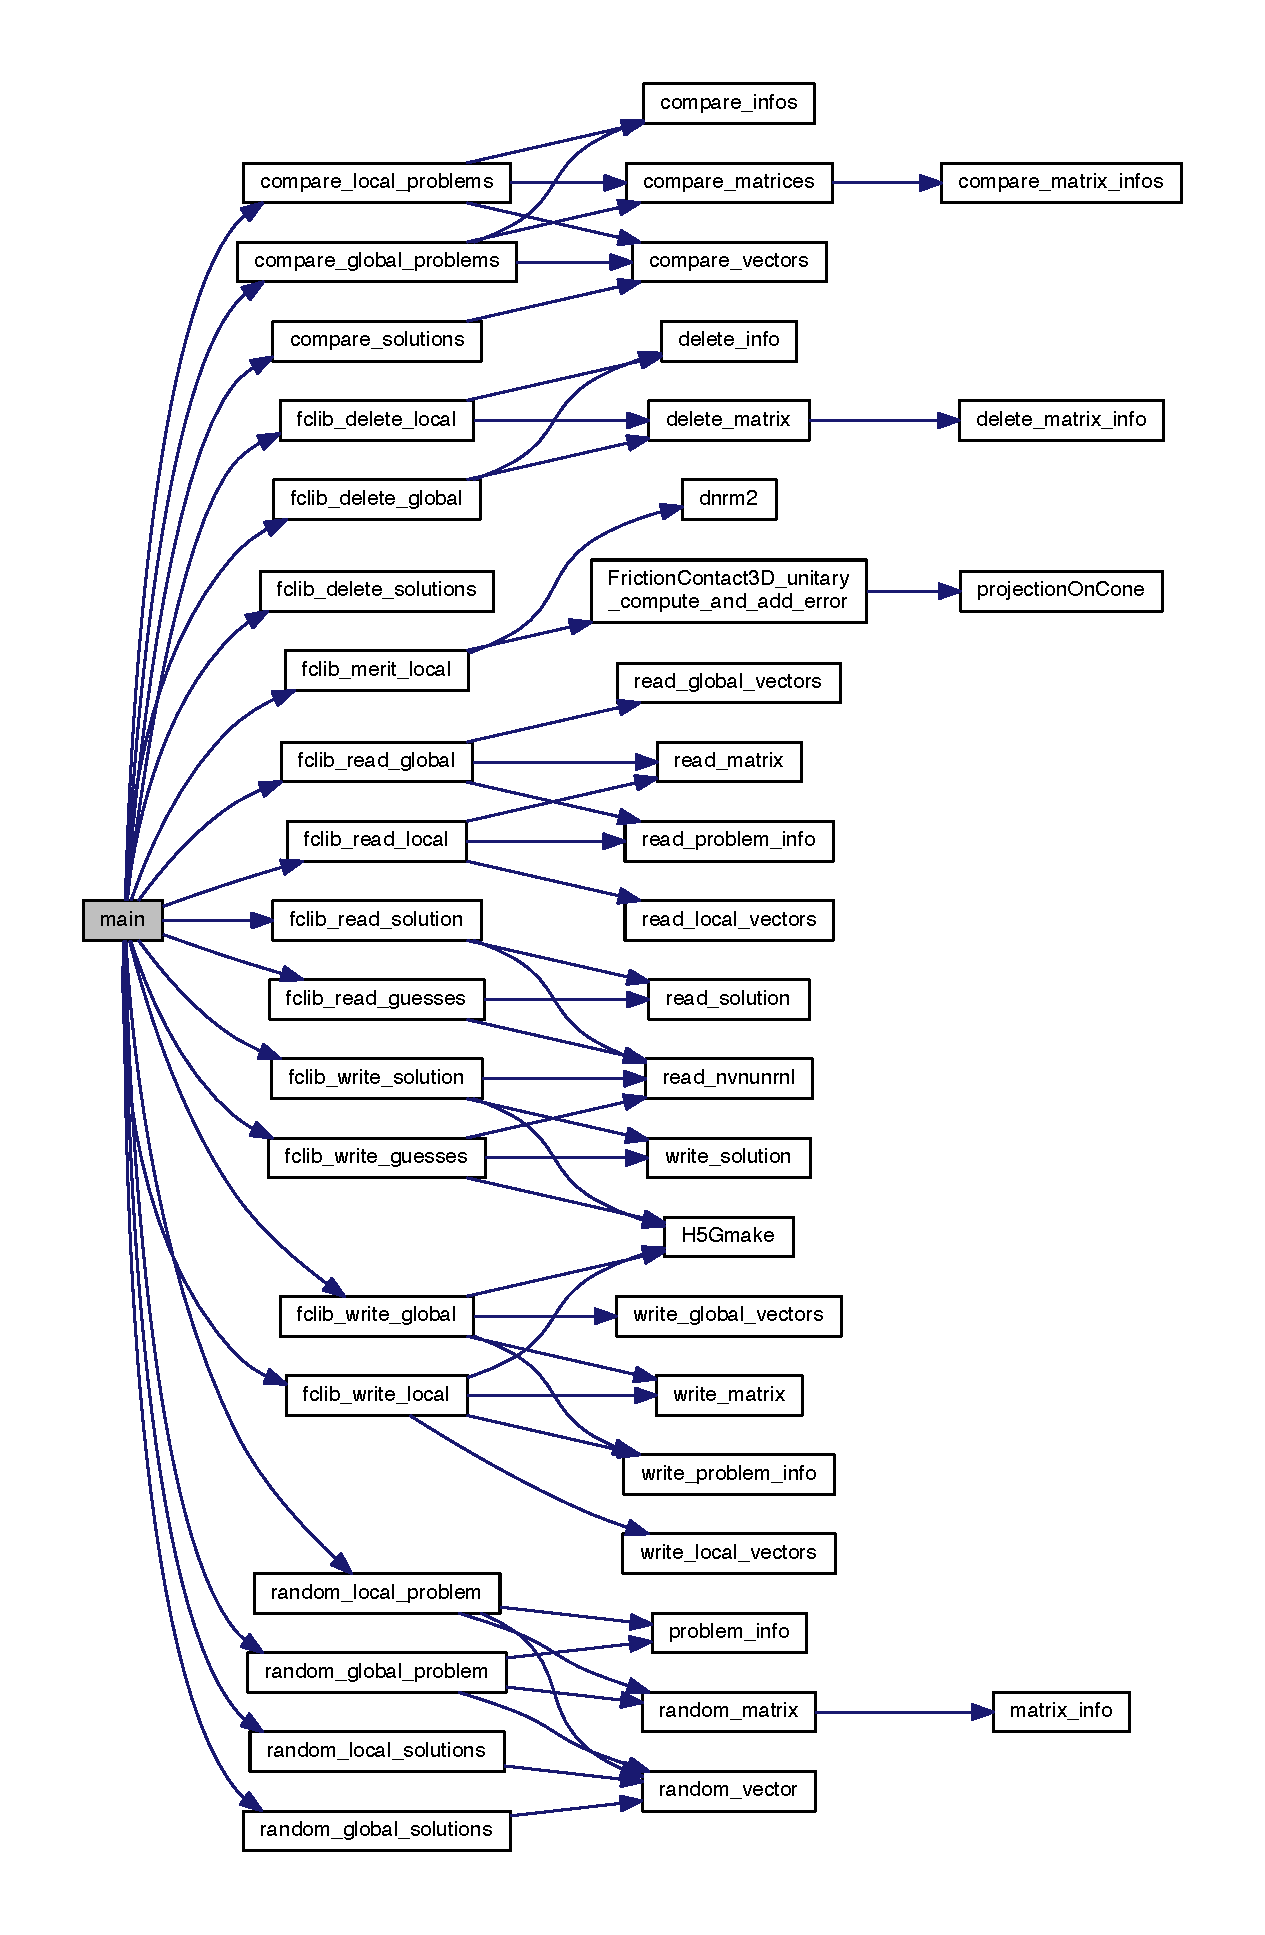
\includegraphics[width=350pt]{fctst_8c_a3c04138a5bfe5d72780bb7e82a18e627_cgraph}
\end{center}
\end{figure}



\hypertarget{fctst__merit_8c}{}\subsection{fctst\+\_\+merit.\+c File Reference}
\label{fctst__merit_8c}\index{fctst\+\_\+merit.\+c@{fctst\+\_\+merit.\+c}}
{\ttfamily \#include $<$string.\+h$>$}\\*
{\ttfamily \#include $<$stdlib.\+h$>$}\\*
{\ttfamily \#include $<$stdio.\+h$>$}\\*
{\ttfamily \#include $<$time.\+h$>$}\\*
{\ttfamily \#include \char`\"{}fclib.\+h\char`\"{}}\\*
{\ttfamily \#include \char`\"{}fcint.\+h\char`\"{}}\\*
Include dependency graph for fctst\+\_\+merit.\+c\+:\nopagebreak
\begin{figure}[H]
\begin{center}
\leavevmode
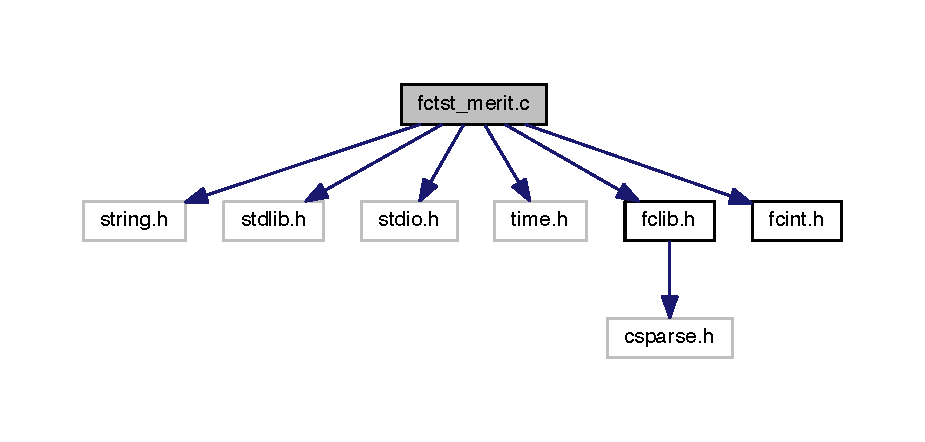
\includegraphics[width=350pt]{fctst__merit_8c__incl}
\end{center}
\end{figure}
\subsubsection*{Functions}
\begin{DoxyCompactItemize}
\item 
static struct \hyperlink{structfclib__matrix__info}{fclib\+\_\+matrix\+\_\+info} $\ast$ \hyperlink{fctst__merit_8c_a5317d629631ea1f011ac56be9ea38b38}{matrix\+\_\+info} (struct \hyperlink{structfclib__matrix}{fclib\+\_\+matrix} $\ast$mat, char $\ast$comment)
\item 
static struct \hyperlink{structfclib__matrix}{fclib\+\_\+matrix} $\ast$ \hyperlink{fctst__merit_8c_a6416171cd1c45fcd483d9f8d72b4d074}{random\+\_\+matrix} (int m, int n)
\item 
static double $\ast$ \hyperlink{fctst__merit_8c_a999ad2a7d7f608315a960fead29ed28b}{random\+\_\+vector} (int n)
\item 
static struct \hyperlink{structfclib__info}{fclib\+\_\+info} $\ast$ \hyperlink{fctst__merit_8c_abacfc09e4ebacd539b34abc2eb6dd26c}{problem\+\_\+info} (char $\ast$title, char $\ast$desc, char $\ast$math)
\item 
static struct \hyperlink{structfclib__global}{fclib\+\_\+global} $\ast$ \hyperlink{fctst__merit_8c_a6bef941fe768030a414543381d847b64}{random\+\_\+global\+\_\+problem} (int global\+\_\+dofs, int contact\+\_\+points, int neq)
\item 
static struct \hyperlink{structfclib__solution}{fclib\+\_\+solution} $\ast$ \hyperlink{fctst__merit_8c_a7aad52ff7bfb95ad106f406bc9c55e58}{random\+\_\+global\+\_\+solutions} (struct \hyperlink{structfclib__global}{fclib\+\_\+global} $\ast$problem, int count)
\item 
static struct \hyperlink{structfclib__local}{fclib\+\_\+local} $\ast$ \hyperlink{fctst__merit_8c_aa112c21ec93e39bb3d3f0461aaa17eec}{random\+\_\+local\+\_\+problem} (int contact\+\_\+points, int neq)
\item 
static struct \hyperlink{structfclib__solution}{fclib\+\_\+solution} $\ast$ \hyperlink{fctst__merit_8c_ab80ee715851eb0c92913d5687498c2d7}{random\+\_\+local\+\_\+solutions} (struct \hyperlink{structfclib__local}{fclib\+\_\+local} $\ast$problem, int count)
\item 
static int \hyperlink{fctst__merit_8c_afe507e5b61471a838e743fe8966e1dde}{compare\+\_\+matrix\+\_\+infos} (struct \hyperlink{structfclib__matrix__info}{fclib\+\_\+matrix\+\_\+info} $\ast$a, struct \hyperlink{structfclib__matrix__info}{fclib\+\_\+matrix\+\_\+info} $\ast$b)
\item 
static int \hyperlink{fctst__merit_8c_ae337371ca0bad878ee90abcb775e94b6}{compare\+\_\+matrices} (char $\ast$name, struct \hyperlink{structfclib__matrix}{fclib\+\_\+matrix} $\ast$a, struct \hyperlink{structfclib__matrix}{fclib\+\_\+matrix} $\ast$b)
\item 
static int \hyperlink{fctst__merit_8c_a67077fe8eef8d36f1bc54695d4e38b07}{compare\+\_\+vectors} (char $\ast$name, int n, double $\ast$a, double $\ast$b)
\item 
static int \hyperlink{fctst__merit_8c_a9616c18dc1480beb7de7875405ba8a69}{compare\+\_\+infos} (struct \hyperlink{structfclib__info}{fclib\+\_\+info} $\ast$a, struct \hyperlink{structfclib__info}{fclib\+\_\+info} $\ast$b)
\item 
static int \hyperlink{fctst__merit_8c_aeadef34f0fb9a9e71e98d044a21fb51f}{compare\+\_\+global\+\_\+problems} (struct \hyperlink{structfclib__global}{fclib\+\_\+global} $\ast$a, struct \hyperlink{structfclib__global}{fclib\+\_\+global} $\ast$b)
\item 
static int \hyperlink{fctst__merit_8c_ab0228efafe00f19b638a3f5cdd03eb98}{compare\+\_\+local\+\_\+problems} (struct \hyperlink{structfclib__local}{fclib\+\_\+local} $\ast$a, struct \hyperlink{structfclib__local}{fclib\+\_\+local} $\ast$b)
\item 
static int \hyperlink{fctst__merit_8c_a65196cbffb155f5d40ff33f2d1b825c2}{compare\+\_\+solutions} (struct \hyperlink{structfclib__solution}{fclib\+\_\+solution} $\ast$a, struct \hyperlink{structfclib__solution}{fclib\+\_\+solution} $\ast$b, int nv, int nr, int nl)
\item 
int \hyperlink{fctst__merit_8c_a3c04138a5bfe5d72780bb7e82a18e627}{main} (int argc, char $\ast$$\ast$argv)
\end{DoxyCompactItemize}


\subsubsection{Function Documentation}
\hypertarget{fctst__merit_8c_a5317d629631ea1f011ac56be9ea38b38}{}\index{fctst\+\_\+merit.\+c@{fctst\+\_\+merit.\+c}!matrix\+\_\+info@{matrix\+\_\+info}}
\index{matrix\+\_\+info@{matrix\+\_\+info}!fctst\+\_\+merit.\+c@{fctst\+\_\+merit.\+c}}
\paragraph[{matrix\+\_\+info(struct fclib\+\_\+matrix $\ast$mat, char $\ast$comment)}]{\setlength{\rightskip}{0pt plus 5cm}static struct {\bf fclib\+\_\+matrix\+\_\+info}$\ast$ matrix\+\_\+info (
\begin{DoxyParamCaption}
\item[{struct {\bf fclib\+\_\+matrix} $\ast$}]{mat, }
\item[{char $\ast$}]{comment}
\end{DoxyParamCaption}
)\hspace{0.3cm}{\ttfamily [static]}}\label{fctst__merit_8c_a5317d629631ea1f011ac56be9ea38b38}


Definition at line 33 of file fctst\+\_\+merit.\+c.



References fclib\+\_\+matrix\+\_\+info\+::comment, fclib\+\_\+matrix\+\_\+info\+::conditioning, fclib\+\_\+matrix\+\_\+info\+::determinant, fclib\+\_\+matrix\+::m, M\+M, and fclib\+\_\+matrix\+\_\+info\+::rank.



Referenced by random\+\_\+matrix().

\hypertarget{fctst__merit_8c_a6416171cd1c45fcd483d9f8d72b4d074}{}\index{fctst\+\_\+merit.\+c@{fctst\+\_\+merit.\+c}!random\+\_\+matrix@{random\+\_\+matrix}}
\index{random\+\_\+matrix@{random\+\_\+matrix}!fctst\+\_\+merit.\+c@{fctst\+\_\+merit.\+c}}
\paragraph[{random\+\_\+matrix(int m, int n)}]{\setlength{\rightskip}{0pt plus 5cm}static struct {\bf fclib\+\_\+matrix}$\ast$ random\+\_\+matrix (
\begin{DoxyParamCaption}
\item[{int}]{m, }
\item[{int}]{n}
\end{DoxyParamCaption}
)\hspace{0.3cm}{\ttfamily [static]}}\label{fctst__merit_8c_a6416171cd1c45fcd483d9f8d72b4d074}


Definition at line 48 of file fctst\+\_\+merit.\+c.



References fclib\+\_\+matrix\+::i, fclib\+\_\+matrix\+::info, fclib\+\_\+matrix\+::m, matrix\+\_\+info(), M\+M, fclib\+\_\+matrix\+::n, fclib\+\_\+matrix\+::nz, fclib\+\_\+matrix\+::nzmax, fclib\+\_\+matrix\+::p, and fclib\+\_\+matrix\+::x.



Referenced by random\+\_\+global\+\_\+problem(), and random\+\_\+local\+\_\+problem().



Here is the call graph for this function\+:\nopagebreak
\begin{figure}[H]
\begin{center}
\leavevmode
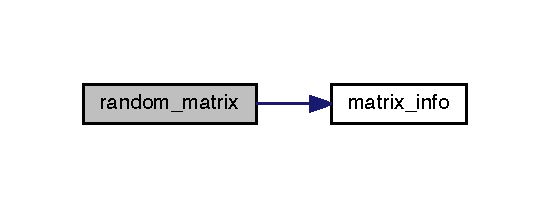
\includegraphics[width=264pt]{fctst__merit_8c_a6416171cd1c45fcd483d9f8d72b4d074_cgraph}
\end{center}
\end{figure}


\hypertarget{fctst__merit_8c_a999ad2a7d7f608315a960fead29ed28b}{}\index{fctst\+\_\+merit.\+c@{fctst\+\_\+merit.\+c}!random\+\_\+vector@{random\+\_\+vector}}
\index{random\+\_\+vector@{random\+\_\+vector}!fctst\+\_\+merit.\+c@{fctst\+\_\+merit.\+c}}
\paragraph[{random\+\_\+vector(int n)}]{\setlength{\rightskip}{0pt plus 5cm}static double$\ast$ random\+\_\+vector (
\begin{DoxyParamCaption}
\item[{int}]{n}
\end{DoxyParamCaption}
)\hspace{0.3cm}{\ttfamily [static]}}\label{fctst__merit_8c_a999ad2a7d7f608315a960fead29ed28b}


Definition at line 91 of file fctst\+\_\+merit.\+c.



References M\+M.



Referenced by random\+\_\+global\+\_\+problem(), random\+\_\+global\+\_\+solutions(), random\+\_\+local\+\_\+problem(), and random\+\_\+local\+\_\+solutions().

\hypertarget{fctst__merit_8c_abacfc09e4ebacd539b34abc2eb6dd26c}{}\index{fctst\+\_\+merit.\+c@{fctst\+\_\+merit.\+c}!problem\+\_\+info@{problem\+\_\+info}}
\index{problem\+\_\+info@{problem\+\_\+info}!fctst\+\_\+merit.\+c@{fctst\+\_\+merit.\+c}}
\paragraph[{problem\+\_\+info(char $\ast$title, char $\ast$desc, char $\ast$math)}]{\setlength{\rightskip}{0pt plus 5cm}static struct {\bf fclib\+\_\+info}$\ast$ problem\+\_\+info (
\begin{DoxyParamCaption}
\item[{char $\ast$}]{title, }
\item[{char $\ast$}]{desc, }
\item[{char $\ast$}]{math}
\end{DoxyParamCaption}
)\hspace{0.3cm}{\ttfamily [static]}}\label{fctst__merit_8c_abacfc09e4ebacd539b34abc2eb6dd26c}


Definition at line 102 of file fctst\+\_\+merit.\+c.



References fclib\+\_\+info\+::description, fclib\+\_\+info\+::math\+\_\+info, M\+M, and fclib\+\_\+info\+::title.



Referenced by random\+\_\+global\+\_\+problem(), and random\+\_\+local\+\_\+problem().

\hypertarget{fctst__merit_8c_a6bef941fe768030a414543381d847b64}{}\index{fctst\+\_\+merit.\+c@{fctst\+\_\+merit.\+c}!random\+\_\+global\+\_\+problem@{random\+\_\+global\+\_\+problem}}
\index{random\+\_\+global\+\_\+problem@{random\+\_\+global\+\_\+problem}!fctst\+\_\+merit.\+c@{fctst\+\_\+merit.\+c}}
\paragraph[{random\+\_\+global\+\_\+problem(int global\+\_\+dofs, int contact\+\_\+points, int neq)}]{\setlength{\rightskip}{0pt plus 5cm}static struct {\bf fclib\+\_\+global}$\ast$ random\+\_\+global\+\_\+problem (
\begin{DoxyParamCaption}
\item[{int}]{global\+\_\+dofs, }
\item[{int}]{contact\+\_\+points, }
\item[{int}]{neq}
\end{DoxyParamCaption}
)\hspace{0.3cm}{\ttfamily [static]}}\label{fctst__merit_8c_a6bef941fe768030a414543381d847b64}


Definition at line 118 of file fctst\+\_\+merit.\+c.



References fclib\+\_\+global\+::b, fclib\+\_\+global\+::f, fclib\+\_\+global\+::\+G, fclib\+\_\+global\+::\+H, fclib\+\_\+global\+::info, fclib\+\_\+global\+::\+M, M\+M, fclib\+\_\+global\+::mu, fclib\+\_\+matrix\+::n, problem\+\_\+info(), random\+\_\+matrix(), random\+\_\+vector(), fclib\+\_\+global\+::spacedim, and fclib\+\_\+global\+::w.



Here is the call graph for this function\+:\nopagebreak
\begin{figure}[H]
\begin{center}
\leavevmode
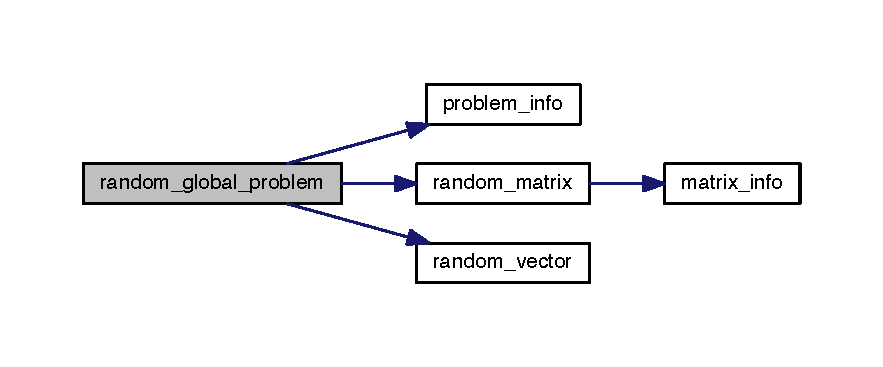
\includegraphics[width=350pt]{fctst__merit_8c_a6bef941fe768030a414543381d847b64_cgraph}
\end{center}
\end{figure}


\hypertarget{fctst__merit_8c_a7aad52ff7bfb95ad106f406bc9c55e58}{}\index{fctst\+\_\+merit.\+c@{fctst\+\_\+merit.\+c}!random\+\_\+global\+\_\+solutions@{random\+\_\+global\+\_\+solutions}}
\index{random\+\_\+global\+\_\+solutions@{random\+\_\+global\+\_\+solutions}!fctst\+\_\+merit.\+c@{fctst\+\_\+merit.\+c}}
\paragraph[{random\+\_\+global\+\_\+solutions(struct fclib\+\_\+global $\ast$problem, int count)}]{\setlength{\rightskip}{0pt plus 5cm}static struct {\bf fclib\+\_\+solution}$\ast$ random\+\_\+global\+\_\+solutions (
\begin{DoxyParamCaption}
\item[{struct {\bf fclib\+\_\+global} $\ast$}]{problem, }
\item[{int}]{count}
\end{DoxyParamCaption}
)\hspace{0.3cm}{\ttfamily [static]}}\label{fctst__merit_8c_a7aad52ff7bfb95ad106f406bc9c55e58}


Definition at line 141 of file fctst\+\_\+merit.\+c.



References fclib\+\_\+global\+::\+G, fclib\+\_\+global\+::\+H, fclib\+\_\+solution\+::l, fclib\+\_\+global\+::\+M, M\+M, fclib\+\_\+matrix\+::n, fclib\+\_\+solution\+::r, random\+\_\+vector(), fclib\+\_\+solution\+::u, and fclib\+\_\+solution\+::v.



Here is the call graph for this function\+:\nopagebreak
\begin{figure}[H]
\begin{center}
\leavevmode
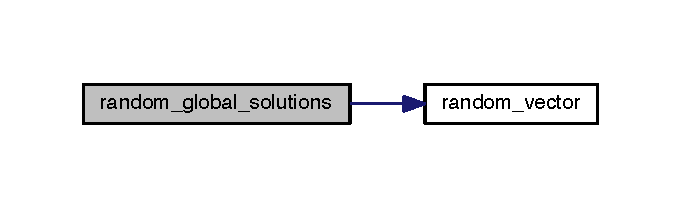
\includegraphics[width=327pt]{fctst__merit_8c_a7aad52ff7bfb95ad106f406bc9c55e58_cgraph}
\end{center}
\end{figure}


\hypertarget{fctst__merit_8c_aa112c21ec93e39bb3d3f0461aaa17eec}{}\index{fctst\+\_\+merit.\+c@{fctst\+\_\+merit.\+c}!random\+\_\+local\+\_\+problem@{random\+\_\+local\+\_\+problem}}
\index{random\+\_\+local\+\_\+problem@{random\+\_\+local\+\_\+problem}!fctst\+\_\+merit.\+c@{fctst\+\_\+merit.\+c}}
\paragraph[{random\+\_\+local\+\_\+problem(int contact\+\_\+points, int neq)}]{\setlength{\rightskip}{0pt plus 5cm}static struct {\bf fclib\+\_\+local}$\ast$ random\+\_\+local\+\_\+problem (
\begin{DoxyParamCaption}
\item[{int}]{contact\+\_\+points, }
\item[{int}]{neq}
\end{DoxyParamCaption}
)\hspace{0.3cm}{\ttfamily [static]}}\label{fctst__merit_8c_aa112c21ec93e39bb3d3f0461aaa17eec}


Definition at line 161 of file fctst\+\_\+merit.\+c.



References fclib\+\_\+local\+::info, M\+M, fclib\+\_\+local\+::mu, problem\+\_\+info(), fclib\+\_\+local\+::q, fclib\+\_\+local\+::\+R, random\+\_\+matrix(), random\+\_\+vector(), fclib\+\_\+local\+::s, fclib\+\_\+local\+::spacedim, fclib\+\_\+local\+::\+V, and fclib\+\_\+local\+::\+W.



Here is the call graph for this function\+:\nopagebreak
\begin{figure}[H]
\begin{center}
\leavevmode
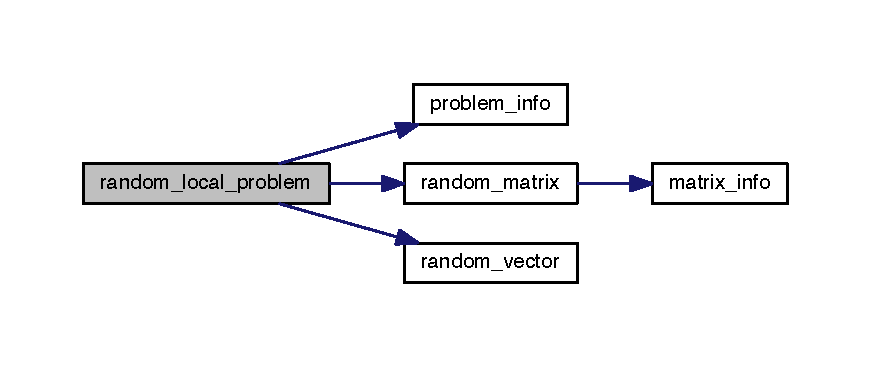
\includegraphics[width=350pt]{fctst__merit_8c_aa112c21ec93e39bb3d3f0461aaa17eec_cgraph}
\end{center}
\end{figure}


\hypertarget{fctst__merit_8c_ab80ee715851eb0c92913d5687498c2d7}{}\index{fctst\+\_\+merit.\+c@{fctst\+\_\+merit.\+c}!random\+\_\+local\+\_\+solutions@{random\+\_\+local\+\_\+solutions}}
\index{random\+\_\+local\+\_\+solutions@{random\+\_\+local\+\_\+solutions}!fctst\+\_\+merit.\+c@{fctst\+\_\+merit.\+c}}
\paragraph[{random\+\_\+local\+\_\+solutions(struct fclib\+\_\+local $\ast$problem, int count)}]{\setlength{\rightskip}{0pt plus 5cm}static struct {\bf fclib\+\_\+solution}$\ast$ random\+\_\+local\+\_\+solutions (
\begin{DoxyParamCaption}
\item[{struct {\bf fclib\+\_\+local} $\ast$}]{problem, }
\item[{int}]{count}
\end{DoxyParamCaption}
)\hspace{0.3cm}{\ttfamily [static]}}\label{fctst__merit_8c_ab80ee715851eb0c92913d5687498c2d7}


Definition at line 189 of file fctst\+\_\+merit.\+c.



References fclib\+\_\+solution\+::l, M\+M, fclib\+\_\+matrix\+::n, fclib\+\_\+local\+::\+R, fclib\+\_\+solution\+::r, random\+\_\+vector(), fclib\+\_\+solution\+::u, fclib\+\_\+solution\+::v, and fclib\+\_\+local\+::\+W.



Here is the call graph for this function\+:\nopagebreak
\begin{figure}[H]
\begin{center}
\leavevmode
\includegraphics[width=321pt]{fctst__merit_8c_ab80ee715851eb0c92913d5687498c2d7_cgraph}
\end{center}
\end{figure}


\hypertarget{fctst__merit_8c_afe507e5b61471a838e743fe8966e1dde}{}\index{fctst\+\_\+merit.\+c@{fctst\+\_\+merit.\+c}!compare\+\_\+matrix\+\_\+infos@{compare\+\_\+matrix\+\_\+infos}}
\index{compare\+\_\+matrix\+\_\+infos@{compare\+\_\+matrix\+\_\+infos}!fctst\+\_\+merit.\+c@{fctst\+\_\+merit.\+c}}
\paragraph[{compare\+\_\+matrix\+\_\+infos(struct fclib\+\_\+matrix\+\_\+info $\ast$a, struct fclib\+\_\+matrix\+\_\+info $\ast$b)}]{\setlength{\rightskip}{0pt plus 5cm}static int compare\+\_\+matrix\+\_\+infos (
\begin{DoxyParamCaption}
\item[{struct {\bf fclib\+\_\+matrix\+\_\+info} $\ast$}]{a, }
\item[{struct {\bf fclib\+\_\+matrix\+\_\+info} $\ast$}]{b}
\end{DoxyParamCaption}
)\hspace{0.3cm}{\ttfamily [static]}}\label{fctst__merit_8c_afe507e5b61471a838e743fe8966e1dde}


Definition at line 209 of file fctst\+\_\+merit.\+c.



References fclib\+\_\+matrix\+\_\+info\+::comment, fclib\+\_\+matrix\+\_\+info\+::conditioning, fclib\+\_\+matrix\+\_\+info\+::determinant, and fclib\+\_\+matrix\+\_\+info\+::rank.



Referenced by compare\+\_\+matrices().

\hypertarget{fctst__merit_8c_ae337371ca0bad878ee90abcb775e94b6}{}\index{fctst\+\_\+merit.\+c@{fctst\+\_\+merit.\+c}!compare\+\_\+matrices@{compare\+\_\+matrices}}
\index{compare\+\_\+matrices@{compare\+\_\+matrices}!fctst\+\_\+merit.\+c@{fctst\+\_\+merit.\+c}}
\paragraph[{compare\+\_\+matrices(char $\ast$name, struct fclib\+\_\+matrix $\ast$a, struct fclib\+\_\+matrix $\ast$b)}]{\setlength{\rightskip}{0pt plus 5cm}static int compare\+\_\+matrices (
\begin{DoxyParamCaption}
\item[{char $\ast$}]{name, }
\item[{struct {\bf fclib\+\_\+matrix} $\ast$}]{a, }
\item[{struct {\bf fclib\+\_\+matrix} $\ast$}]{b}
\end{DoxyParamCaption}
)\hspace{0.3cm}{\ttfamily [static]}}\label{fctst__merit_8c_ae337371ca0bad878ee90abcb775e94b6}


Definition at line 222 of file fctst\+\_\+merit.\+c.



References compare\+\_\+matrix\+\_\+infos(), fclib\+\_\+matrix\+::i, fclib\+\_\+matrix\+::info, fclib\+\_\+matrix\+::m, fclib\+\_\+matrix\+::n, fclib\+\_\+matrix\+::nz, fclib\+\_\+matrix\+::nzmax, fclib\+\_\+matrix\+::p, and fclib\+\_\+matrix\+::x.



Referenced by compare\+\_\+global\+\_\+problems(), and compare\+\_\+local\+\_\+problems().



Here is the call graph for this function\+:\nopagebreak
\begin{figure}[H]
\begin{center}
\leavevmode
\includegraphics[width=330pt]{fctst__merit_8c_ae337371ca0bad878ee90abcb775e94b6_cgraph}
\end{center}
\end{figure}


\hypertarget{fctst__merit_8c_a67077fe8eef8d36f1bc54695d4e38b07}{}\index{fctst\+\_\+merit.\+c@{fctst\+\_\+merit.\+c}!compare\+\_\+vectors@{compare\+\_\+vectors}}
\index{compare\+\_\+vectors@{compare\+\_\+vectors}!fctst\+\_\+merit.\+c@{fctst\+\_\+merit.\+c}}
\paragraph[{compare\+\_\+vectors(char $\ast$name, int n, double $\ast$a, double $\ast$b)}]{\setlength{\rightskip}{0pt plus 5cm}static int compare\+\_\+vectors (
\begin{DoxyParamCaption}
\item[{char $\ast$}]{name, }
\item[{int}]{n, }
\item[{double $\ast$}]{a, }
\item[{double $\ast$}]{b}
\end{DoxyParamCaption}
)\hspace{0.3cm}{\ttfamily [static]}}\label{fctst__merit_8c_a67077fe8eef8d36f1bc54695d4e38b07}


Definition at line 327 of file fctst\+\_\+merit.\+c.



Referenced by compare\+\_\+global\+\_\+problems(), compare\+\_\+local\+\_\+problems(), and compare\+\_\+solutions().

\hypertarget{fctst__merit_8c_a9616c18dc1480beb7de7875405ba8a69}{}\index{fctst\+\_\+merit.\+c@{fctst\+\_\+merit.\+c}!compare\+\_\+infos@{compare\+\_\+infos}}
\index{compare\+\_\+infos@{compare\+\_\+infos}!fctst\+\_\+merit.\+c@{fctst\+\_\+merit.\+c}}
\paragraph[{compare\+\_\+infos(struct fclib\+\_\+info $\ast$a, struct fclib\+\_\+info $\ast$b)}]{\setlength{\rightskip}{0pt plus 5cm}static int compare\+\_\+infos (
\begin{DoxyParamCaption}
\item[{struct {\bf fclib\+\_\+info} $\ast$}]{a, }
\item[{struct {\bf fclib\+\_\+info} $\ast$}]{b}
\end{DoxyParamCaption}
)\hspace{0.3cm}{\ttfamily [static]}}\label{fctst__merit_8c_a9616c18dc1480beb7de7875405ba8a69}


Definition at line 347 of file fctst\+\_\+merit.\+c.



References fclib\+\_\+info\+::description, fclib\+\_\+info\+::math\+\_\+info, and fclib\+\_\+info\+::title.



Referenced by compare\+\_\+global\+\_\+problems(), and compare\+\_\+local\+\_\+problems().

\hypertarget{fctst__merit_8c_aeadef34f0fb9a9e71e98d044a21fb51f}{}\index{fctst\+\_\+merit.\+c@{fctst\+\_\+merit.\+c}!compare\+\_\+global\+\_\+problems@{compare\+\_\+global\+\_\+problems}}
\index{compare\+\_\+global\+\_\+problems@{compare\+\_\+global\+\_\+problems}!fctst\+\_\+merit.\+c@{fctst\+\_\+merit.\+c}}
\paragraph[{compare\+\_\+global\+\_\+problems(struct fclib\+\_\+global $\ast$a, struct fclib\+\_\+global $\ast$b)}]{\setlength{\rightskip}{0pt plus 5cm}static int compare\+\_\+global\+\_\+problems (
\begin{DoxyParamCaption}
\item[{struct {\bf fclib\+\_\+global} $\ast$}]{a, }
\item[{struct {\bf fclib\+\_\+global} $\ast$}]{b}
\end{DoxyParamCaption}
)\hspace{0.3cm}{\ttfamily [static]}}\label{fctst__merit_8c_aeadef34f0fb9a9e71e98d044a21fb51f}


Definition at line 359 of file fctst\+\_\+merit.\+c.



References fclib\+\_\+global\+::b, compare\+\_\+infos(), compare\+\_\+matrices(), compare\+\_\+vectors(), fclib\+\_\+global\+::f, fclib\+\_\+global\+::\+G, fclib\+\_\+global\+::\+H, fclib\+\_\+global\+::info, fclib\+\_\+matrix\+::m, fclib\+\_\+global\+::\+M, fclib\+\_\+global\+::mu, fclib\+\_\+matrix\+::n, fclib\+\_\+global\+::spacedim, and fclib\+\_\+global\+::w.



Here is the call graph for this function\+:\nopagebreak
\begin{figure}[H]
\begin{center}
\leavevmode
\includegraphics[width=350pt]{fctst__merit_8c_aeadef34f0fb9a9e71e98d044a21fb51f_cgraph}
\end{center}
\end{figure}


\hypertarget{fctst__merit_8c_ab0228efafe00f19b638a3f5cdd03eb98}{}\index{fctst\+\_\+merit.\+c@{fctst\+\_\+merit.\+c}!compare\+\_\+local\+\_\+problems@{compare\+\_\+local\+\_\+problems}}
\index{compare\+\_\+local\+\_\+problems@{compare\+\_\+local\+\_\+problems}!fctst\+\_\+merit.\+c@{fctst\+\_\+merit.\+c}}
\paragraph[{compare\+\_\+local\+\_\+problems(struct fclib\+\_\+local $\ast$a, struct fclib\+\_\+local $\ast$b)}]{\setlength{\rightskip}{0pt plus 5cm}static int compare\+\_\+local\+\_\+problems (
\begin{DoxyParamCaption}
\item[{struct {\bf fclib\+\_\+local} $\ast$}]{a, }
\item[{struct {\bf fclib\+\_\+local} $\ast$}]{b}
\end{DoxyParamCaption}
)\hspace{0.3cm}{\ttfamily [static]}}\label{fctst__merit_8c_ab0228efafe00f19b638a3f5cdd03eb98}


Definition at line 375 of file fctst\+\_\+merit.\+c.



References compare\+\_\+infos(), compare\+\_\+matrices(), compare\+\_\+vectors(), fclib\+\_\+local\+::info, fclib\+\_\+local\+::mu, fclib\+\_\+matrix\+::n, fclib\+\_\+local\+::q, fclib\+\_\+local\+::\+R, fclib\+\_\+local\+::s, fclib\+\_\+local\+::spacedim, fclib\+\_\+local\+::\+V, and fclib\+\_\+local\+::\+W.



Here is the call graph for this function\+:\nopagebreak
\begin{figure}[H]
\begin{center}
\leavevmode
\includegraphics[width=350pt]{fctst__merit_8c_ab0228efafe00f19b638a3f5cdd03eb98_cgraph}
\end{center}
\end{figure}


\hypertarget{fctst__merit_8c_a65196cbffb155f5d40ff33f2d1b825c2}{}\index{fctst\+\_\+merit.\+c@{fctst\+\_\+merit.\+c}!compare\+\_\+solutions@{compare\+\_\+solutions}}
\index{compare\+\_\+solutions@{compare\+\_\+solutions}!fctst\+\_\+merit.\+c@{fctst\+\_\+merit.\+c}}
\paragraph[{compare\+\_\+solutions(struct fclib\+\_\+solution $\ast$a, struct fclib\+\_\+solution $\ast$b, int nv, int nr, int nl)}]{\setlength{\rightskip}{0pt plus 5cm}static int compare\+\_\+solutions (
\begin{DoxyParamCaption}
\item[{struct {\bf fclib\+\_\+solution} $\ast$}]{a, }
\item[{struct {\bf fclib\+\_\+solution} $\ast$}]{b, }
\item[{int}]{nv, }
\item[{int}]{nr, }
\item[{int}]{nl}
\end{DoxyParamCaption}
)\hspace{0.3cm}{\ttfamily [static]}}\label{fctst__merit_8c_a65196cbffb155f5d40ff33f2d1b825c2}


Definition at line 390 of file fctst\+\_\+merit.\+c.



References compare\+\_\+vectors(), fclib\+\_\+solution\+::l, fclib\+\_\+solution\+::r, fclib\+\_\+solution\+::u, and fclib\+\_\+solution\+::v.



Here is the call graph for this function\+:\nopagebreak
\begin{figure}[H]
\begin{center}
\leavevmode
\includegraphics[width=309pt]{fctst__merit_8c_a65196cbffb155f5d40ff33f2d1b825c2_cgraph}
\end{center}
\end{figure}


\hypertarget{fctst__merit_8c_a3c04138a5bfe5d72780bb7e82a18e627}{}\index{fctst\+\_\+merit.\+c@{fctst\+\_\+merit.\+c}!main@{main}}
\index{main@{main}!fctst\+\_\+merit.\+c@{fctst\+\_\+merit.\+c}}
\paragraph[{main(int argc, char $\ast$$\ast$argv)}]{\setlength{\rightskip}{0pt plus 5cm}int main (
\begin{DoxyParamCaption}
\item[{int}]{argc, }
\item[{char $\ast$$\ast$}]{argv}
\end{DoxyParamCaption}
)}\label{fctst__merit_8c_a3c04138a5bfe5d72780bb7e82a18e627}


Definition at line 400 of file fctst\+\_\+merit.\+c.



References fclib\+\_\+delete\+\_\+global(), fclib\+\_\+delete\+\_\+local(), fclib\+\_\+delete\+\_\+solutions(), fclib\+\_\+merit\+\_\+global(), fclib\+\_\+merit\+\_\+local(), fclib\+\_\+read\+\_\+global(), fclib\+\_\+read\+\_\+guesses(), fclib\+\_\+read\+\_\+local(), fclib\+\_\+read\+\_\+solution(), and M\+E\+R\+I\+T\+\_\+1.



Here is the call graph for this function\+:\nopagebreak
\begin{figure}[H]
\begin{center}
\leavevmode
\includegraphics[width=350pt]{fctst__merit_8c_a3c04138a5bfe5d72780bb7e82a18e627_cgraph}
\end{center}
\end{figure}



\hypertarget{mainpage_8doxygen}{}\subsection{mainpage.\+doxygen File Reference}
\label{mainpage_8doxygen}\index{mainpage.\+doxygen@{mainpage.\+doxygen}}

%--- End generated contents ---

% Index
\newpage
\phantomsection
\clearemptydoublepage
\addcontentsline{toc}{section}{Index}
\printindex

\end{document}
